\documentclass[10pt]{imta}

\usepackage{config}

\title[PhD Defense of Léo Lavaur]{Improving Intrusion Detection in Distributed Systems with Federated Learning}

\subtitle{}

\author[Léo Lavaur]{\textbf{Léo Lavaur}}

\institute{IMT Atlantique $\cdot$ IRISA (SOTERN)}

\date{Rennes, October 7\textsuperscript{th}, 2024}

\titlegraphic{%
  \raisebox{-0.5\height}{
\includegraphics[height=\logosize,keepaspectratio]{logos/imt-atlantique.pdf}}%
  \raisebox{-0.5\height}{
\includegraphics[height=.75\logosize,keepaspectratio]{logos/cybercniGB.pdf}}%
  \raisebox{-0.5\height}{
\includegraphics[height=.7\logosize,keepaspectratio]{logos/irisa.jpg}}%
}

\subject{Federated Learning; Intrusion Detection; Byzantine; Cross-evaluation; Similarity; Clustering; Reputation Systems; Trust; Heterogeneity}

%%%%%%%%%%%%%%%%%%%%%%%%%%%%%%%%%%%%%%%%%%%%%%%%%%%%%%%%%%%%%%%%%%%%%%%%%%%%%%%%
%%%%                            DOCUMENT CONTENT                            %%%%
%%%%%%%%%%%%%%%%%%%%%%%%%%%%%%%%%%%%%%%%%%%%%%%%%%%%%%%%%%%%%%%%%%%%%%%%%%%%%%%%

\begin{document}

\jury{
  \begin{tabular}{@{}l@{\hspace{1ex}}l@{}}
    \textbf{Reviewers}:   & Anne-Marie Kermarrec    $\cdot$ EPFL \\
                          & Eric Totel              $\cdot$ Télécom SudParis \\
    \textbf{Examiners}:   & Sonia Ben Mokhtar       $\cdot$ CNRS \\
                          & Pierre-François Gimenez $\cdot$ Inria \\
                          & Vincent Nicomette       $\cdot$ INSA Toulouse \\
    \textbf{Supervisors}: & Fabien Autrel           $\cdot$ IMT Atlantique \\
                          & Marc-Oliver Pahl        $\cdot$ IMT Atlantique \\
    \textbf{Director}:    & Yann Busnel             $\cdot$ IMT \\
  \end{tabular}
}

\maketitle

% ------------------------------------------------------------------------------

\section*{Introduction}

\begin{frame}{Information Security}
  \begin{figure}
    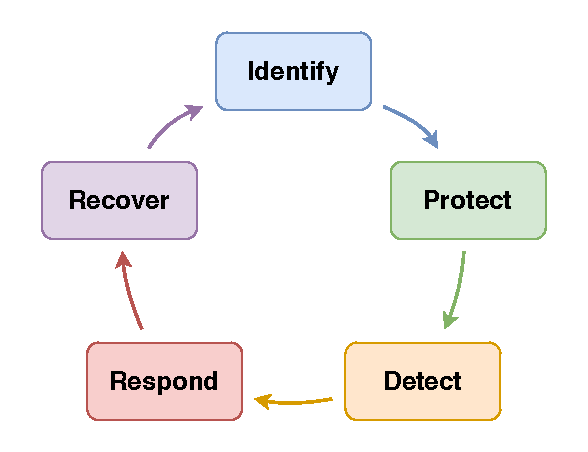
\includegraphics[width=.4\linewidth]{figures/intro/security.drawio.pdf}
    \caption*{The security life-cycle \cite{nationalinstituteofstandardsandtechnology_NISTCybersecurityFramework_2024}.}
  \end{figure}

  \fcitefootnote{nationalinstituteofstandardsandtechnology_NISTCybersecurityFramework_2024}
\end{frame}

\begin{frame}{The Need for Collaboration}
  \centering
  \foreach \i in {1,...,4} {%
    \includegraphics<\i>[width=.9\textwidth]{figures/intro/collab/collab-\i.drawio.pdf}%
  }
\end{frame}

\begin{frame}{Collaboration in Cybersecurity}
  \begin{columns}
    \begin{column}{.6\textwidth}
      \begin{itemize}
        \item Collaboration pushed by:
        \begin{itemize}[<+->]
          \item common interest (\eg, inter-SOCs\footnotemark);
          \item national agencies (\eg, NIST, ENISA, ANSSI);
          \item regulation (\eg, private-public information sharing in NIS2).
        \end{itemize}
      \end{itemize}
    \end{column}
    \begin{column}{.4\textwidth}
      \centering
      %\includegraphics<+>[width=\linewidth]{figures/intro/security-collab.drawio.pdf}%
      \includegraphics<+->[width=\linewidth]{figures/intro/security-focus.drawio.pdf}%
    \end{column}
  \end{columns}
  
  \onslide<+>
  \centering
  \begin{minipage}{.6\textwidth}    
    \begin{block}{Intrusion Detection System (IDS)}
      \medskip
      IDSs monitor the behavior of a system to detect malicious activities.
    \end{block}
  \end{minipage}

  \footnotetext{Security Operational Center.}
\end{frame}


\begin{frame}{Machine Learning for Intrusion Detection}
  \bigskip
  \only<+>{}%
  \begin{itemize}
    \item Various types of algorithms: \alert<+->{supervised}, unsupervised, semi-supervised, reinforcement learning, \etc.
    \item Great performance with Deep Learning (DL)\dots{}
    \onslide<+->
    \emph{on public datasets at least}.
  \end{itemize}
  \bigskip
  
  \onslide<+->
  \begin{columns}
    \begin{column}{0.4\textwidth}
        \textbf{Challenges of local training:}
        \begin{itemize}
          \item not enough labelled data;
          \item risk of local bias or skewed data distribution.
          % \item inefficient against new attacks, especially \alert{supervised} approaches.
        \end{itemize}
    \end{column}

    \begin{column}{0.6\textwidth}
      \begin{figure}
        \centering
        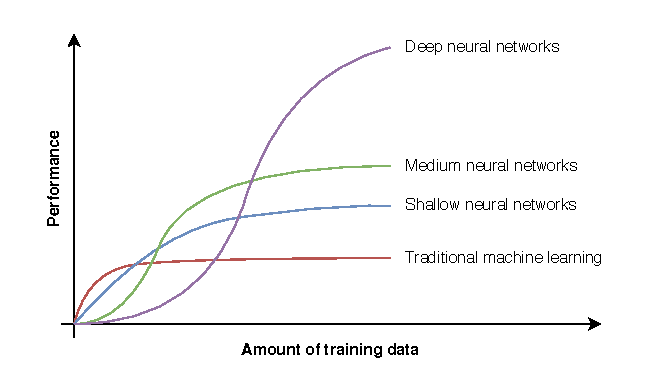
\includegraphics[width=\linewidth]{figures/intro/ml-perf}
      \end{figure}
    \end{column}
  \end{columns}
\end{frame}

\begin{frame}{Data Sharing to the Rescue?}
% TODO:
% pas assez de données, faisons un pot commun !
% oui mais non :
% - confidentialité des données 
% - confiance dans le point de collecte
% - confiance dnas le processus d'apprentissage
% - pas de modèle de detection sans serveur
\begin{columns}
  \begin{column}{0.5\textwidth}
    \centering
    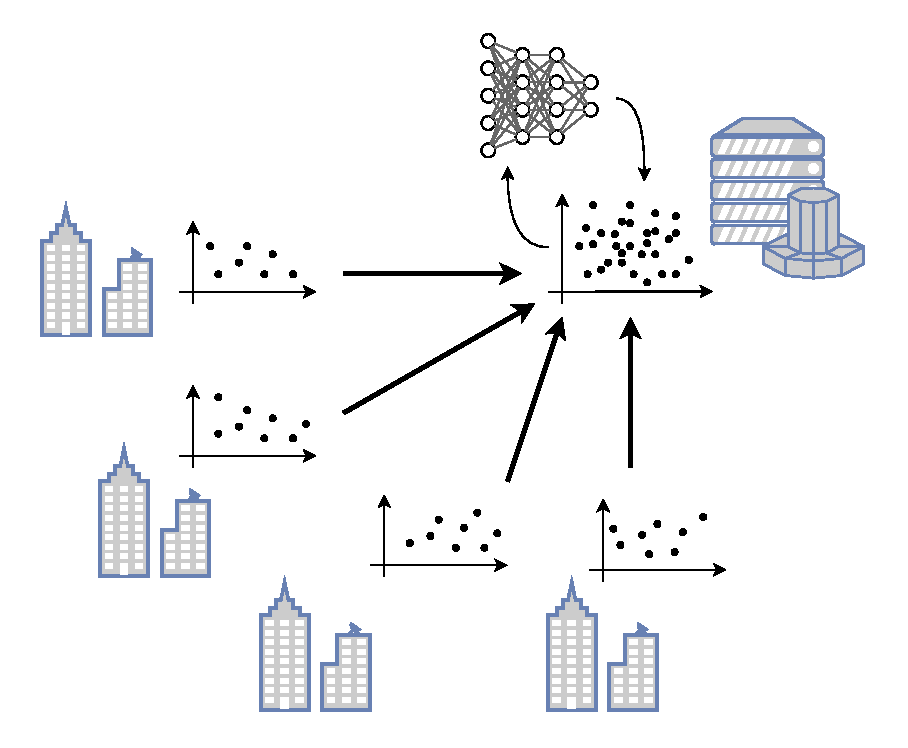
\includegraphics[width=\linewidth]{figures/intro/collab.pdf}
  \end{column}
  \begin{column}{0.5\textwidth}
    \textbf{Let's pool our data!}\pause{} \textbf{Although\dots}
    \begin{itemize}
      \item Privacy concerns.
      \item Lack of trust in the data holder.
      \item Lack of trust in the learning process.
      %\item Lack of incentives.
      \item \dots
    \end{itemize}
  \end{column}
\end{columns}
\end{frame}


\begin{frame}{Scaling Intrusion Detection}

  \textbf{Federated Learning (FL)}
  
  \begin{itemize}[<+->]
    \item Novel-\emph{ish} distributed ML paradigm (Google)~\autocite{mcmahan_Communicationefficientlearningdeep_2017}.
    \item Distributed clients can train a common model without sharing their training data.
    \item \alert{Privacy-preserving}: high level of abstraction for the shared models preventing data leakage.
  \end{itemize}

  \fcitefootnote{mcmahan_Communicationefficientlearningdeep_2017}
\end{frame}


\begin{frame}{FL Fundamentals}

  \begin{figure}
    \centering
    \foreach \i in {1,...,7} {%
      \includegraphics<\i>[width=.75\linewidth]{./figures/intro/fl/\i.pdf}%
    }
    \caption{Typical FL workflow, applied to NIDSs.}
  \end{figure}
\end{frame}


% \begin{frame}{FL for NIDSs}

%   \textbf{Benefits}
%   \begin{itemize}[<+->]
%     \item Virtually extended dataset with Horizontal FL.
%     \begin{itemize}[<1->]
%       \item Better generalization.
%       \item Reduced risk of overfitting or local bias.
%     \end{itemize}
    

%     \item Effectively share knowledge (\eg, on specific classes, instances) between participants
%     \begin{itemize}[<1->]
%       \item Share the knowledge about a new attack~\autocite{lavaur_icdcs_demo_2024};
%       \item Improve the characterization of specific devices; \dots
%     \end{itemize}

%     \only<2>{\fcitefootnote{lavaur_icdcs_demo_2024}}

%   \end{itemize}
% \end{frame}


\begin{frame}{Case Study}
  \bigskip
  \textbf{Collaborative Intrusion Detection between Distributed Organizations}
  \begin{itemize}[<+->]
    \item Each organization has its own NIDS\footnote{Network-based IDS} and monitors an information system.
    \item Objective: improve their local detection performance.
    \item Means: \alert{expert knowledge} (\ie, datasets) and \alert{computing resources} (\ie, model training).
  \end{itemize}
  \medskip
  \pause
  \begin{figure}
    \centering
    \makebox[\textwidth][c]{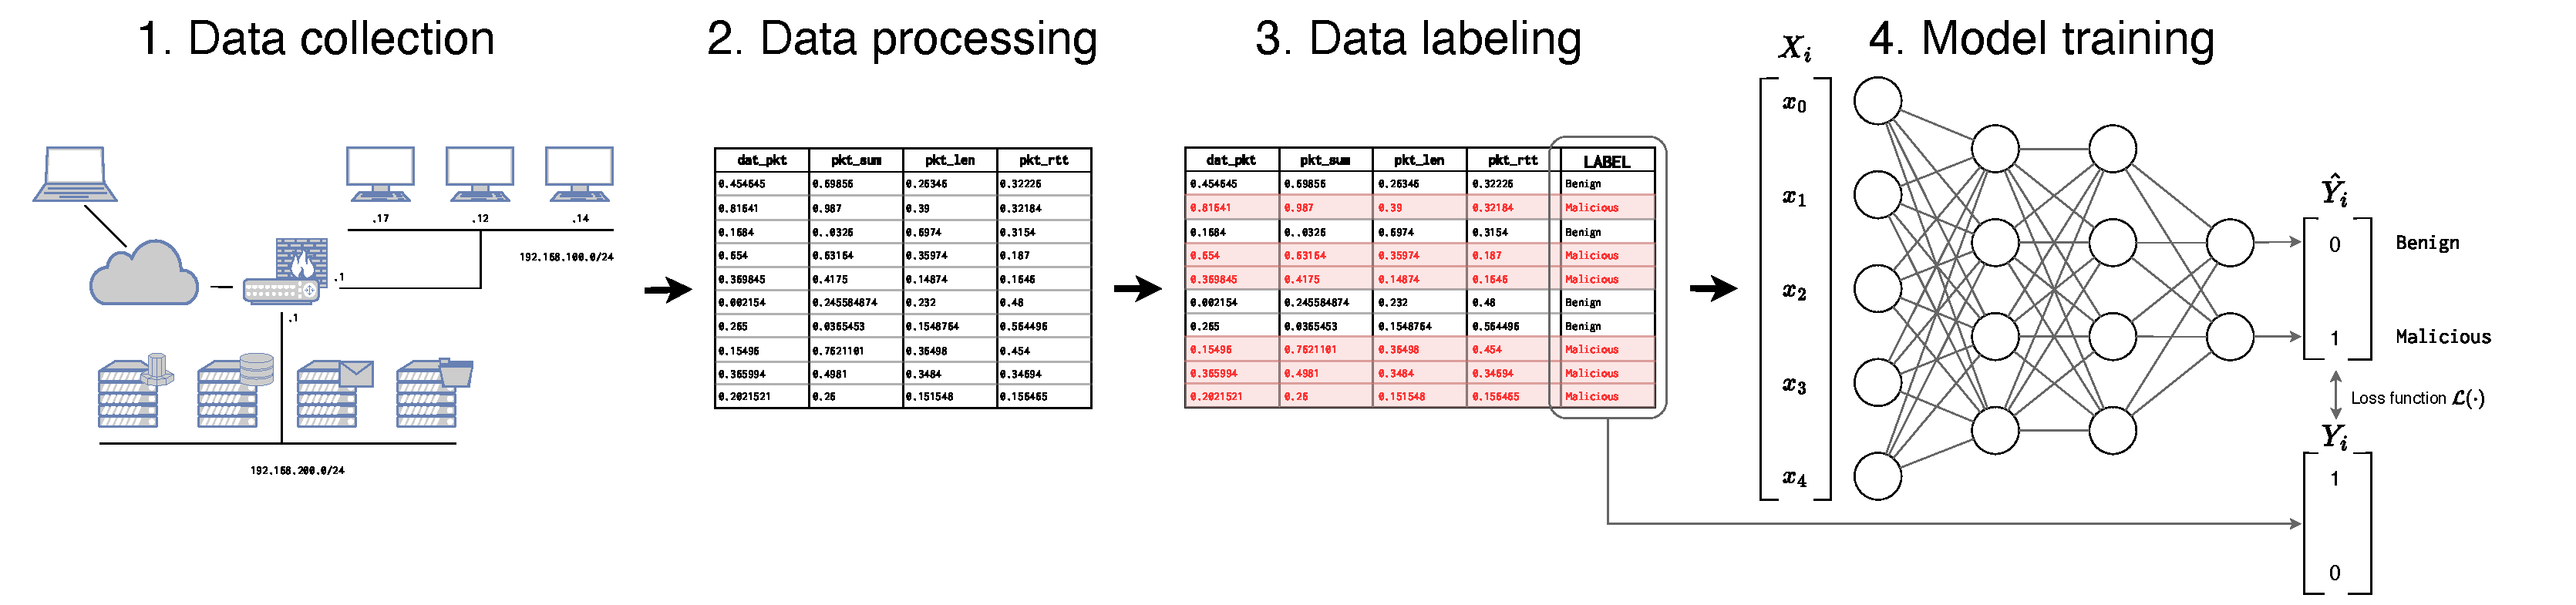
\includegraphics[width=.9\textwidth]{figures/intro/mlp-workflow.pdf}}
    \caption{Typical workflow for ML-based NIDSs.}
  \end{figure}
\end{frame}


\begin{frame}{Case Study -- Generalization}
  \textbf{A cross-silo use case}~\cite{kairouz_AdvancesOpenProblems_2021}:
  \begin{itemize}
    \item few clients (\ie, 10--100);
    \item substantial amount of data, high heterogeneity;
    \item high availability, significant computing resources.
  \end{itemize}
\end{frame}



\begin{frame}{Systematic Literature Review}
  
  \begin{columns}
    \begin{column}{.45\textwidth}
      % \textbf{Systematic Literature Review (SLR)}~\autocite{lavaur_tnsm_2022}
      % \begin{itemize}
      %   \item Booming topic over the last 4--5 years.
      %   \item Very heterogeneous venues and communities.
      % \end{itemize}

      \textbf{Challenges from the Literature}~\autocite{lavaur_tnsm_2022}
      \begin{itemize}[<+->]
        \item \emph{Functionality}: \chqual[6-]{performance}, \chhetero[6-]{heterogeneity}, \chtransfer[6-]{transferability}, self-defense, and self-healing.
        \item \emph{Deployment}: \chunknown[6-]{adaptability} and \chdecent[6-]{scalability}.
        \item \emph{Security and reliability}: \chpoison[6-]{security}, privacy, \chpoison[6-]{trust}, and reputation.
        \item \emph{Experimentation}: evaluation.
      \end{itemize}
    \end{column}
    \begin{column}{.55\textwidth}
      \only<5-6>{%
        \begin{figure}
          \centering
          \resizebox{\linewidth}{!}{%% Creator: Matplotlib, PGF backend
%%
%% To include the figure in your LaTeX document, write
%%   \input{<filename>.pgf}
%%
%% Make sure the required packages are loaded in your preamble
%%   \usepackage{pgf}
%%
%% Also ensure that all the required font packages are loaded; for instance,
%% the lmodern package is sometimes necessary when using math font.
%%   \usepackage{lmodern}
%%
%% Figures using additional raster images can only be included by \input if
%% they are in the same directory as the main LaTeX file. For loading figures
%% from other directories you can use the `import` package
%%   \usepackage{import}
%%
%% and then include the figures with
%%   \import{<path to file>}{<filename>.pgf}
%%
%% Matplotlib used the following preamble
%%   \def\mathdefault#1{#1}
%%   \everymath=\expandafter{\the\everymath\displaystyle}
%%   
%%   \usepackage{fontspec}
%%   \makeatletter\@ifpackageloaded{underscore}{}{\usepackage[strings]{underscore}}\makeatother
%%
\begingroup%
\makeatletter%
\begin{pgfpicture}%
\pgfpathrectangle{\pgfpointorigin}{\pgfqpoint{3.140876in}{1.985768in}}%
\pgfusepath{use as bounding box, clip}%
\begin{pgfscope}%
\pgfsetbuttcap%
\pgfsetmiterjoin%
\definecolor{currentfill}{rgb}{1.000000,1.000000,1.000000}%
\pgfsetfillcolor{currentfill}%
\pgfsetlinewidth{0.000000pt}%
\definecolor{currentstroke}{rgb}{1.000000,1.000000,1.000000}%
\pgfsetstrokecolor{currentstroke}%
\pgfsetdash{}{0pt}%
\pgfpathmoveto{\pgfqpoint{0.000000in}{0.000000in}}%
\pgfpathlineto{\pgfqpoint{3.140876in}{0.000000in}}%
\pgfpathlineto{\pgfqpoint{3.140876in}{1.985768in}}%
\pgfpathlineto{\pgfqpoint{0.000000in}{1.985768in}}%
\pgfpathlineto{\pgfqpoint{0.000000in}{0.000000in}}%
\pgfpathclose%
\pgfusepath{fill}%
\end{pgfscope}%
\begin{pgfscope}%
\pgfsetbuttcap%
\pgfsetmiterjoin%
\definecolor{currentfill}{rgb}{1.000000,1.000000,1.000000}%
\pgfsetfillcolor{currentfill}%
\pgfsetlinewidth{0.000000pt}%
\definecolor{currentstroke}{rgb}{0.000000,0.000000,0.000000}%
\pgfsetstrokecolor{currentstroke}%
\pgfsetstrokeopacity{0.000000}%
\pgfsetdash{}{0pt}%
\pgfpathmoveto{\pgfqpoint{0.374222in}{0.433222in}}%
\pgfpathlineto{\pgfqpoint{1.568043in}{0.433222in}}%
\pgfpathlineto{\pgfqpoint{1.568043in}{1.885768in}}%
\pgfpathlineto{\pgfqpoint{0.374222in}{1.885768in}}%
\pgfpathlineto{\pgfqpoint{0.374222in}{0.433222in}}%
\pgfpathclose%
\pgfusepath{fill}%
\end{pgfscope}%
\begin{pgfscope}%
\pgfpathrectangle{\pgfqpoint{0.374222in}{0.433222in}}{\pgfqpoint{1.193820in}{1.452545in}}%
\pgfusepath{clip}%
\pgfsetbuttcap%
\pgfsetmiterjoin%
\definecolor{currentfill}{rgb}{0.121569,0.466667,0.705882}%
\pgfsetfillcolor{currentfill}%
\pgfsetlinewidth{0.000000pt}%
\definecolor{currentstroke}{rgb}{0.000000,0.000000,0.000000}%
\pgfsetstrokecolor{currentstroke}%
\pgfsetstrokeopacity{0.000000}%
\pgfsetdash{}{0pt}%
\pgfpathmoveto{\pgfqpoint{0.391277in}{0.433222in}}%
\pgfpathlineto{\pgfqpoint{0.527713in}{0.433222in}}%
\pgfpathlineto{\pgfqpoint{0.527713in}{0.433222in}}%
\pgfpathlineto{\pgfqpoint{0.391277in}{0.433222in}}%
\pgfpathlineto{\pgfqpoint{0.391277in}{0.433222in}}%
\pgfpathclose%
\pgfusepath{fill}%
\end{pgfscope}%
\begin{pgfscope}%
\pgfpathrectangle{\pgfqpoint{0.374222in}{0.433222in}}{\pgfqpoint{1.193820in}{1.452545in}}%
\pgfusepath{clip}%
\pgfsetbuttcap%
\pgfsetmiterjoin%
\definecolor{currentfill}{rgb}{0.121569,0.466667,0.705882}%
\pgfsetfillcolor{currentfill}%
\pgfsetlinewidth{0.000000pt}%
\definecolor{currentstroke}{rgb}{0.000000,0.000000,0.000000}%
\pgfsetstrokecolor{currentstroke}%
\pgfsetstrokeopacity{0.000000}%
\pgfsetdash{}{0pt}%
\pgfpathmoveto{\pgfqpoint{0.561823in}{0.433222in}}%
\pgfpathlineto{\pgfqpoint{0.698259in}{0.433222in}}%
\pgfpathlineto{\pgfqpoint{0.698259in}{0.433222in}}%
\pgfpathlineto{\pgfqpoint{0.561823in}{0.433222in}}%
\pgfpathlineto{\pgfqpoint{0.561823in}{0.433222in}}%
\pgfpathclose%
\pgfusepath{fill}%
\end{pgfscope}%
\begin{pgfscope}%
\pgfpathrectangle{\pgfqpoint{0.374222in}{0.433222in}}{\pgfqpoint{1.193820in}{1.452545in}}%
\pgfusepath{clip}%
\pgfsetbuttcap%
\pgfsetmiterjoin%
\definecolor{currentfill}{rgb}{0.121569,0.466667,0.705882}%
\pgfsetfillcolor{currentfill}%
\pgfsetlinewidth{0.000000pt}%
\definecolor{currentstroke}{rgb}{0.000000,0.000000,0.000000}%
\pgfsetstrokecolor{currentstroke}%
\pgfsetstrokeopacity{0.000000}%
\pgfsetdash{}{0pt}%
\pgfpathmoveto{\pgfqpoint{0.732368in}{0.433222in}}%
\pgfpathlineto{\pgfqpoint{0.868805in}{0.433222in}}%
\pgfpathlineto{\pgfqpoint{0.868805in}{0.433222in}}%
\pgfpathlineto{\pgfqpoint{0.732368in}{0.433222in}}%
\pgfpathlineto{\pgfqpoint{0.732368in}{0.433222in}}%
\pgfpathclose%
\pgfusepath{fill}%
\end{pgfscope}%
\begin{pgfscope}%
\pgfpathrectangle{\pgfqpoint{0.374222in}{0.433222in}}{\pgfqpoint{1.193820in}{1.452545in}}%
\pgfusepath{clip}%
\pgfsetbuttcap%
\pgfsetmiterjoin%
\definecolor{currentfill}{rgb}{0.121569,0.466667,0.705882}%
\pgfsetfillcolor{currentfill}%
\pgfsetlinewidth{0.000000pt}%
\definecolor{currentstroke}{rgb}{0.000000,0.000000,0.000000}%
\pgfsetstrokecolor{currentstroke}%
\pgfsetstrokeopacity{0.000000}%
\pgfsetdash{}{0pt}%
\pgfpathmoveto{\pgfqpoint{0.902914in}{0.433222in}}%
\pgfpathlineto{\pgfqpoint{1.039351in}{0.433222in}}%
\pgfpathlineto{\pgfqpoint{1.039351in}{0.433222in}}%
\pgfpathlineto{\pgfqpoint{0.902914in}{0.433222in}}%
\pgfpathlineto{\pgfqpoint{0.902914in}{0.433222in}}%
\pgfpathclose%
\pgfusepath{fill}%
\end{pgfscope}%
\begin{pgfscope}%
\pgfpathrectangle{\pgfqpoint{0.374222in}{0.433222in}}{\pgfqpoint{1.193820in}{1.452545in}}%
\pgfusepath{clip}%
\pgfsetbuttcap%
\pgfsetmiterjoin%
\definecolor{currentfill}{rgb}{0.121569,0.466667,0.705882}%
\pgfsetfillcolor{currentfill}%
\pgfsetlinewidth{0.000000pt}%
\definecolor{currentstroke}{rgb}{0.000000,0.000000,0.000000}%
\pgfsetstrokecolor{currentstroke}%
\pgfsetstrokeopacity{0.000000}%
\pgfsetdash{}{0pt}%
\pgfpathmoveto{\pgfqpoint{1.073460in}{0.433222in}}%
\pgfpathlineto{\pgfqpoint{1.209897in}{0.433222in}}%
\pgfpathlineto{\pgfqpoint{1.209897in}{0.462043in}}%
\pgfpathlineto{\pgfqpoint{1.073460in}{0.462043in}}%
\pgfpathlineto{\pgfqpoint{1.073460in}{0.433222in}}%
\pgfpathclose%
\pgfusepath{fill}%
\end{pgfscope}%
\begin{pgfscope}%
\pgfpathrectangle{\pgfqpoint{0.374222in}{0.433222in}}{\pgfqpoint{1.193820in}{1.452545in}}%
\pgfusepath{clip}%
\pgfsetbuttcap%
\pgfsetmiterjoin%
\definecolor{currentfill}{rgb}{0.121569,0.466667,0.705882}%
\pgfsetfillcolor{currentfill}%
\pgfsetlinewidth{0.000000pt}%
\definecolor{currentstroke}{rgb}{0.000000,0.000000,0.000000}%
\pgfsetstrokecolor{currentstroke}%
\pgfsetstrokeopacity{0.000000}%
\pgfsetdash{}{0pt}%
\pgfpathmoveto{\pgfqpoint{1.244006in}{0.433222in}}%
\pgfpathlineto{\pgfqpoint{1.380442in}{0.433222in}}%
\pgfpathlineto{\pgfqpoint{1.380442in}{0.480116in}}%
\pgfpathlineto{\pgfqpoint{1.244006in}{0.480116in}}%
\pgfpathlineto{\pgfqpoint{1.244006in}{0.433222in}}%
\pgfpathclose%
\pgfusepath{fill}%
\end{pgfscope}%
\begin{pgfscope}%
\pgfpathrectangle{\pgfqpoint{0.374222in}{0.433222in}}{\pgfqpoint{1.193820in}{1.452545in}}%
\pgfusepath{clip}%
\pgfsetbuttcap%
\pgfsetmiterjoin%
\definecolor{currentfill}{rgb}{0.121569,0.466667,0.705882}%
\pgfsetfillcolor{currentfill}%
\pgfsetlinewidth{0.000000pt}%
\definecolor{currentstroke}{rgb}{0.000000,0.000000,0.000000}%
\pgfsetstrokecolor{currentstroke}%
\pgfsetstrokeopacity{0.000000}%
\pgfsetdash{}{0pt}%
\pgfpathmoveto{\pgfqpoint{1.414551in}{0.433222in}}%
\pgfpathlineto{\pgfqpoint{1.550988in}{0.433222in}}%
\pgfpathlineto{\pgfqpoint{1.550988in}{0.548504in}}%
\pgfpathlineto{\pgfqpoint{1.414551in}{0.548504in}}%
\pgfpathlineto{\pgfqpoint{1.414551in}{0.433222in}}%
\pgfpathclose%
\pgfusepath{fill}%
\end{pgfscope}%
\begin{pgfscope}%
\pgfpathrectangle{\pgfqpoint{0.374222in}{0.433222in}}{\pgfqpoint{1.193820in}{1.452545in}}%
\pgfusepath{clip}%
\pgfsetbuttcap%
\pgfsetmiterjoin%
\definecolor{currentfill}{rgb}{1.000000,0.498039,0.054902}%
\pgfsetfillcolor{currentfill}%
\pgfsetlinewidth{0.000000pt}%
\definecolor{currentstroke}{rgb}{0.000000,0.000000,0.000000}%
\pgfsetstrokecolor{currentstroke}%
\pgfsetstrokeopacity{0.000000}%
\pgfsetdash{}{0pt}%
\pgfpathmoveto{\pgfqpoint{0.391277in}{0.433222in}}%
\pgfpathlineto{\pgfqpoint{0.527713in}{0.433222in}}%
\pgfpathlineto{\pgfqpoint{0.527713in}{0.433222in}}%
\pgfpathlineto{\pgfqpoint{0.391277in}{0.433222in}}%
\pgfpathlineto{\pgfqpoint{0.391277in}{0.433222in}}%
\pgfpathclose%
\pgfusepath{fill}%
\end{pgfscope}%
\begin{pgfscope}%
\pgfpathrectangle{\pgfqpoint{0.374222in}{0.433222in}}{\pgfqpoint{1.193820in}{1.452545in}}%
\pgfusepath{clip}%
\pgfsetbuttcap%
\pgfsetmiterjoin%
\definecolor{currentfill}{rgb}{1.000000,0.498039,0.054902}%
\pgfsetfillcolor{currentfill}%
\pgfsetlinewidth{0.000000pt}%
\definecolor{currentstroke}{rgb}{0.000000,0.000000,0.000000}%
\pgfsetstrokecolor{currentstroke}%
\pgfsetstrokeopacity{0.000000}%
\pgfsetdash{}{0pt}%
\pgfpathmoveto{\pgfqpoint{0.561823in}{0.433222in}}%
\pgfpathlineto{\pgfqpoint{0.698259in}{0.433222in}}%
\pgfpathlineto{\pgfqpoint{0.698259in}{0.709898in}}%
\pgfpathlineto{\pgfqpoint{0.561823in}{0.709898in}}%
\pgfpathlineto{\pgfqpoint{0.561823in}{0.433222in}}%
\pgfpathclose%
\pgfusepath{fill}%
\end{pgfscope}%
\begin{pgfscope}%
\pgfpathrectangle{\pgfqpoint{0.374222in}{0.433222in}}{\pgfqpoint{1.193820in}{1.452545in}}%
\pgfusepath{clip}%
\pgfsetbuttcap%
\pgfsetmiterjoin%
\definecolor{currentfill}{rgb}{1.000000,0.498039,0.054902}%
\pgfsetfillcolor{currentfill}%
\pgfsetlinewidth{0.000000pt}%
\definecolor{currentstroke}{rgb}{0.000000,0.000000,0.000000}%
\pgfsetstrokecolor{currentstroke}%
\pgfsetstrokeopacity{0.000000}%
\pgfsetdash{}{0pt}%
\pgfpathmoveto{\pgfqpoint{0.732368in}{0.433222in}}%
\pgfpathlineto{\pgfqpoint{0.868805in}{0.433222in}}%
\pgfpathlineto{\pgfqpoint{0.868805in}{0.433222in}}%
\pgfpathlineto{\pgfqpoint{0.732368in}{0.433222in}}%
\pgfpathlineto{\pgfqpoint{0.732368in}{0.433222in}}%
\pgfpathclose%
\pgfusepath{fill}%
\end{pgfscope}%
\begin{pgfscope}%
\pgfpathrectangle{\pgfqpoint{0.374222in}{0.433222in}}{\pgfqpoint{1.193820in}{1.452545in}}%
\pgfusepath{clip}%
\pgfsetbuttcap%
\pgfsetmiterjoin%
\definecolor{currentfill}{rgb}{1.000000,0.498039,0.054902}%
\pgfsetfillcolor{currentfill}%
\pgfsetlinewidth{0.000000pt}%
\definecolor{currentstroke}{rgb}{0.000000,0.000000,0.000000}%
\pgfsetstrokecolor{currentstroke}%
\pgfsetstrokeopacity{0.000000}%
\pgfsetdash{}{0pt}%
\pgfpathmoveto{\pgfqpoint{0.902914in}{0.433222in}}%
\pgfpathlineto{\pgfqpoint{1.039351in}{0.433222in}}%
\pgfpathlineto{\pgfqpoint{1.039351in}{0.433222in}}%
\pgfpathlineto{\pgfqpoint{0.902914in}{0.433222in}}%
\pgfpathlineto{\pgfqpoint{0.902914in}{0.433222in}}%
\pgfpathclose%
\pgfusepath{fill}%
\end{pgfscope}%
\begin{pgfscope}%
\pgfpathrectangle{\pgfqpoint{0.374222in}{0.433222in}}{\pgfqpoint{1.193820in}{1.452545in}}%
\pgfusepath{clip}%
\pgfsetbuttcap%
\pgfsetmiterjoin%
\definecolor{currentfill}{rgb}{1.000000,0.498039,0.054902}%
\pgfsetfillcolor{currentfill}%
\pgfsetlinewidth{0.000000pt}%
\definecolor{currentstroke}{rgb}{0.000000,0.000000,0.000000}%
\pgfsetstrokecolor{currentstroke}%
\pgfsetstrokeopacity{0.000000}%
\pgfsetdash{}{0pt}%
\pgfpathmoveto{\pgfqpoint{1.073460in}{0.462043in}}%
\pgfpathlineto{\pgfqpoint{1.209897in}{0.462043in}}%
\pgfpathlineto{\pgfqpoint{1.209897in}{0.490863in}}%
\pgfpathlineto{\pgfqpoint{1.073460in}{0.490863in}}%
\pgfpathlineto{\pgfqpoint{1.073460in}{0.462043in}}%
\pgfpathclose%
\pgfusepath{fill}%
\end{pgfscope}%
\begin{pgfscope}%
\pgfpathrectangle{\pgfqpoint{0.374222in}{0.433222in}}{\pgfqpoint{1.193820in}{1.452545in}}%
\pgfusepath{clip}%
\pgfsetbuttcap%
\pgfsetmiterjoin%
\definecolor{currentfill}{rgb}{1.000000,0.498039,0.054902}%
\pgfsetfillcolor{currentfill}%
\pgfsetlinewidth{0.000000pt}%
\definecolor{currentstroke}{rgb}{0.000000,0.000000,0.000000}%
\pgfsetstrokecolor{currentstroke}%
\pgfsetstrokeopacity{0.000000}%
\pgfsetdash{}{0pt}%
\pgfpathmoveto{\pgfqpoint{1.244006in}{0.480116in}}%
\pgfpathlineto{\pgfqpoint{1.380442in}{0.480116in}}%
\pgfpathlineto{\pgfqpoint{1.380442in}{0.527010in}}%
\pgfpathlineto{\pgfqpoint{1.244006in}{0.527010in}}%
\pgfpathlineto{\pgfqpoint{1.244006in}{0.480116in}}%
\pgfpathclose%
\pgfusepath{fill}%
\end{pgfscope}%
\begin{pgfscope}%
\pgfpathrectangle{\pgfqpoint{0.374222in}{0.433222in}}{\pgfqpoint{1.193820in}{1.452545in}}%
\pgfusepath{clip}%
\pgfsetbuttcap%
\pgfsetmiterjoin%
\definecolor{currentfill}{rgb}{1.000000,0.498039,0.054902}%
\pgfsetfillcolor{currentfill}%
\pgfsetlinewidth{0.000000pt}%
\definecolor{currentstroke}{rgb}{0.000000,0.000000,0.000000}%
\pgfsetstrokecolor{currentstroke}%
\pgfsetstrokeopacity{0.000000}%
\pgfsetdash{}{0pt}%
\pgfpathmoveto{\pgfqpoint{1.414551in}{0.548504in}}%
\pgfpathlineto{\pgfqpoint{1.550988in}{0.548504in}}%
\pgfpathlineto{\pgfqpoint{1.550988in}{0.548504in}}%
\pgfpathlineto{\pgfqpoint{1.414551in}{0.548504in}}%
\pgfpathlineto{\pgfqpoint{1.414551in}{0.548504in}}%
\pgfpathclose%
\pgfusepath{fill}%
\end{pgfscope}%
\begin{pgfscope}%
\pgfpathrectangle{\pgfqpoint{0.374222in}{0.433222in}}{\pgfqpoint{1.193820in}{1.452545in}}%
\pgfusepath{clip}%
\pgfsetbuttcap%
\pgfsetmiterjoin%
\definecolor{currentfill}{rgb}{0.172549,0.627451,0.172549}%
\pgfsetfillcolor{currentfill}%
\pgfsetlinewidth{0.000000pt}%
\definecolor{currentstroke}{rgb}{0.000000,0.000000,0.000000}%
\pgfsetstrokecolor{currentstroke}%
\pgfsetstrokeopacity{0.000000}%
\pgfsetdash{}{0pt}%
\pgfpathmoveto{\pgfqpoint{0.391277in}{0.433222in}}%
\pgfpathlineto{\pgfqpoint{0.527713in}{0.433222in}}%
\pgfpathlineto{\pgfqpoint{0.527713in}{1.124910in}}%
\pgfpathlineto{\pgfqpoint{0.391277in}{1.124910in}}%
\pgfpathlineto{\pgfqpoint{0.391277in}{0.433222in}}%
\pgfpathclose%
\pgfusepath{fill}%
\end{pgfscope}%
\begin{pgfscope}%
\pgfpathrectangle{\pgfqpoint{0.374222in}{0.433222in}}{\pgfqpoint{1.193820in}{1.452545in}}%
\pgfusepath{clip}%
\pgfsetbuttcap%
\pgfsetmiterjoin%
\definecolor{currentfill}{rgb}{0.172549,0.627451,0.172549}%
\pgfsetfillcolor{currentfill}%
\pgfsetlinewidth{0.000000pt}%
\definecolor{currentstroke}{rgb}{0.000000,0.000000,0.000000}%
\pgfsetstrokecolor{currentstroke}%
\pgfsetstrokeopacity{0.000000}%
\pgfsetdash{}{0pt}%
\pgfpathmoveto{\pgfqpoint{0.561823in}{0.709898in}}%
\pgfpathlineto{\pgfqpoint{0.698259in}{0.709898in}}%
\pgfpathlineto{\pgfqpoint{0.698259in}{0.986573in}}%
\pgfpathlineto{\pgfqpoint{0.561823in}{0.986573in}}%
\pgfpathlineto{\pgfqpoint{0.561823in}{0.709898in}}%
\pgfpathclose%
\pgfusepath{fill}%
\end{pgfscope}%
\begin{pgfscope}%
\pgfpathrectangle{\pgfqpoint{0.374222in}{0.433222in}}{\pgfqpoint{1.193820in}{1.452545in}}%
\pgfusepath{clip}%
\pgfsetbuttcap%
\pgfsetmiterjoin%
\definecolor{currentfill}{rgb}{0.172549,0.627451,0.172549}%
\pgfsetfillcolor{currentfill}%
\pgfsetlinewidth{0.000000pt}%
\definecolor{currentstroke}{rgb}{0.000000,0.000000,0.000000}%
\pgfsetstrokecolor{currentstroke}%
\pgfsetstrokeopacity{0.000000}%
\pgfsetdash{}{0pt}%
\pgfpathmoveto{\pgfqpoint{0.732368in}{0.433222in}}%
\pgfpathlineto{\pgfqpoint{0.868805in}{0.433222in}}%
\pgfpathlineto{\pgfqpoint{0.868805in}{0.709898in}}%
\pgfpathlineto{\pgfqpoint{0.732368in}{0.709898in}}%
\pgfpathlineto{\pgfqpoint{0.732368in}{0.433222in}}%
\pgfpathclose%
\pgfusepath{fill}%
\end{pgfscope}%
\begin{pgfscope}%
\pgfpathrectangle{\pgfqpoint{0.374222in}{0.433222in}}{\pgfqpoint{1.193820in}{1.452545in}}%
\pgfusepath{clip}%
\pgfsetbuttcap%
\pgfsetmiterjoin%
\definecolor{currentfill}{rgb}{0.172549,0.627451,0.172549}%
\pgfsetfillcolor{currentfill}%
\pgfsetlinewidth{0.000000pt}%
\definecolor{currentstroke}{rgb}{0.000000,0.000000,0.000000}%
\pgfsetstrokecolor{currentstroke}%
\pgfsetstrokeopacity{0.000000}%
\pgfsetdash{}{0pt}%
\pgfpathmoveto{\pgfqpoint{0.902914in}{0.433222in}}%
\pgfpathlineto{\pgfqpoint{1.039351in}{0.433222in}}%
\pgfpathlineto{\pgfqpoint{1.039351in}{0.433222in}}%
\pgfpathlineto{\pgfqpoint{0.902914in}{0.433222in}}%
\pgfpathlineto{\pgfqpoint{0.902914in}{0.433222in}}%
\pgfpathclose%
\pgfusepath{fill}%
\end{pgfscope}%
\begin{pgfscope}%
\pgfpathrectangle{\pgfqpoint{0.374222in}{0.433222in}}{\pgfqpoint{1.193820in}{1.452545in}}%
\pgfusepath{clip}%
\pgfsetbuttcap%
\pgfsetmiterjoin%
\definecolor{currentfill}{rgb}{0.172549,0.627451,0.172549}%
\pgfsetfillcolor{currentfill}%
\pgfsetlinewidth{0.000000pt}%
\definecolor{currentstroke}{rgb}{0.000000,0.000000,0.000000}%
\pgfsetstrokecolor{currentstroke}%
\pgfsetstrokeopacity{0.000000}%
\pgfsetdash{}{0pt}%
\pgfpathmoveto{\pgfqpoint{1.073460in}{0.490863in}}%
\pgfpathlineto{\pgfqpoint{1.209897in}{0.490863in}}%
\pgfpathlineto{\pgfqpoint{1.209897in}{0.548504in}}%
\pgfpathlineto{\pgfqpoint{1.073460in}{0.548504in}}%
\pgfpathlineto{\pgfqpoint{1.073460in}{0.490863in}}%
\pgfpathclose%
\pgfusepath{fill}%
\end{pgfscope}%
\begin{pgfscope}%
\pgfpathrectangle{\pgfqpoint{0.374222in}{0.433222in}}{\pgfqpoint{1.193820in}{1.452545in}}%
\pgfusepath{clip}%
\pgfsetbuttcap%
\pgfsetmiterjoin%
\definecolor{currentfill}{rgb}{0.172549,0.627451,0.172549}%
\pgfsetfillcolor{currentfill}%
\pgfsetlinewidth{0.000000pt}%
\definecolor{currentstroke}{rgb}{0.000000,0.000000,0.000000}%
\pgfsetstrokecolor{currentstroke}%
\pgfsetstrokeopacity{0.000000}%
\pgfsetdash{}{0pt}%
\pgfpathmoveto{\pgfqpoint{1.244006in}{0.527010in}}%
\pgfpathlineto{\pgfqpoint{1.380442in}{0.527010in}}%
\pgfpathlineto{\pgfqpoint{1.380442in}{0.550458in}}%
\pgfpathlineto{\pgfqpoint{1.244006in}{0.550458in}}%
\pgfpathlineto{\pgfqpoint{1.244006in}{0.527010in}}%
\pgfpathclose%
\pgfusepath{fill}%
\end{pgfscope}%
\begin{pgfscope}%
\pgfpathrectangle{\pgfqpoint{0.374222in}{0.433222in}}{\pgfqpoint{1.193820in}{1.452545in}}%
\pgfusepath{clip}%
\pgfsetbuttcap%
\pgfsetmiterjoin%
\definecolor{currentfill}{rgb}{0.172549,0.627451,0.172549}%
\pgfsetfillcolor{currentfill}%
\pgfsetlinewidth{0.000000pt}%
\definecolor{currentstroke}{rgb}{0.000000,0.000000,0.000000}%
\pgfsetstrokecolor{currentstroke}%
\pgfsetstrokeopacity{0.000000}%
\pgfsetdash{}{0pt}%
\pgfpathmoveto{\pgfqpoint{1.414551in}{0.548504in}}%
\pgfpathlineto{\pgfqpoint{1.550988in}{0.548504in}}%
\pgfpathlineto{\pgfqpoint{1.550988in}{0.548504in}}%
\pgfpathlineto{\pgfqpoint{1.414551in}{0.548504in}}%
\pgfpathlineto{\pgfqpoint{1.414551in}{0.548504in}}%
\pgfpathclose%
\pgfusepath{fill}%
\end{pgfscope}%
\begin{pgfscope}%
\pgfpathrectangle{\pgfqpoint{0.374222in}{0.433222in}}{\pgfqpoint{1.193820in}{1.452545in}}%
\pgfusepath{clip}%
\pgfsetbuttcap%
\pgfsetmiterjoin%
\definecolor{currentfill}{rgb}{0.839216,0.152941,0.156863}%
\pgfsetfillcolor{currentfill}%
\pgfsetlinewidth{0.000000pt}%
\definecolor{currentstroke}{rgb}{0.000000,0.000000,0.000000}%
\pgfsetstrokecolor{currentstroke}%
\pgfsetstrokeopacity{0.000000}%
\pgfsetdash{}{0pt}%
\pgfpathmoveto{\pgfqpoint{0.391277in}{1.124910in}}%
\pgfpathlineto{\pgfqpoint{0.527713in}{1.124910in}}%
\pgfpathlineto{\pgfqpoint{0.527713in}{1.124910in}}%
\pgfpathlineto{\pgfqpoint{0.391277in}{1.124910in}}%
\pgfpathlineto{\pgfqpoint{0.391277in}{1.124910in}}%
\pgfpathclose%
\pgfusepath{fill}%
\end{pgfscope}%
\begin{pgfscope}%
\pgfpathrectangle{\pgfqpoint{0.374222in}{0.433222in}}{\pgfqpoint{1.193820in}{1.452545in}}%
\pgfusepath{clip}%
\pgfsetbuttcap%
\pgfsetmiterjoin%
\definecolor{currentfill}{rgb}{0.839216,0.152941,0.156863}%
\pgfsetfillcolor{currentfill}%
\pgfsetlinewidth{0.000000pt}%
\definecolor{currentstroke}{rgb}{0.000000,0.000000,0.000000}%
\pgfsetstrokecolor{currentstroke}%
\pgfsetstrokeopacity{0.000000}%
\pgfsetdash{}{0pt}%
\pgfpathmoveto{\pgfqpoint{0.561823in}{0.986573in}}%
\pgfpathlineto{\pgfqpoint{0.698259in}{0.986573in}}%
\pgfpathlineto{\pgfqpoint{0.698259in}{0.986573in}}%
\pgfpathlineto{\pgfqpoint{0.561823in}{0.986573in}}%
\pgfpathlineto{\pgfqpoint{0.561823in}{0.986573in}}%
\pgfpathclose%
\pgfusepath{fill}%
\end{pgfscope}%
\begin{pgfscope}%
\pgfpathrectangle{\pgfqpoint{0.374222in}{0.433222in}}{\pgfqpoint{1.193820in}{1.452545in}}%
\pgfusepath{clip}%
\pgfsetbuttcap%
\pgfsetmiterjoin%
\definecolor{currentfill}{rgb}{0.839216,0.152941,0.156863}%
\pgfsetfillcolor{currentfill}%
\pgfsetlinewidth{0.000000pt}%
\definecolor{currentstroke}{rgb}{0.000000,0.000000,0.000000}%
\pgfsetstrokecolor{currentstroke}%
\pgfsetstrokeopacity{0.000000}%
\pgfsetdash{}{0pt}%
\pgfpathmoveto{\pgfqpoint{0.732368in}{0.709898in}}%
\pgfpathlineto{\pgfqpoint{0.868805in}{0.709898in}}%
\pgfpathlineto{\pgfqpoint{0.868805in}{0.848235in}}%
\pgfpathlineto{\pgfqpoint{0.732368in}{0.848235in}}%
\pgfpathlineto{\pgfqpoint{0.732368in}{0.709898in}}%
\pgfpathclose%
\pgfusepath{fill}%
\end{pgfscope}%
\begin{pgfscope}%
\pgfpathrectangle{\pgfqpoint{0.374222in}{0.433222in}}{\pgfqpoint{1.193820in}{1.452545in}}%
\pgfusepath{clip}%
\pgfsetbuttcap%
\pgfsetmiterjoin%
\definecolor{currentfill}{rgb}{0.839216,0.152941,0.156863}%
\pgfsetfillcolor{currentfill}%
\pgfsetlinewidth{0.000000pt}%
\definecolor{currentstroke}{rgb}{0.000000,0.000000,0.000000}%
\pgfsetstrokecolor{currentstroke}%
\pgfsetstrokeopacity{0.000000}%
\pgfsetdash{}{0pt}%
\pgfpathmoveto{\pgfqpoint{0.902914in}{0.433222in}}%
\pgfpathlineto{\pgfqpoint{1.039351in}{0.433222in}}%
\pgfpathlineto{\pgfqpoint{1.039351in}{0.677347in}}%
\pgfpathlineto{\pgfqpoint{0.902914in}{0.677347in}}%
\pgfpathlineto{\pgfqpoint{0.902914in}{0.433222in}}%
\pgfpathclose%
\pgfusepath{fill}%
\end{pgfscope}%
\begin{pgfscope}%
\pgfpathrectangle{\pgfqpoint{0.374222in}{0.433222in}}{\pgfqpoint{1.193820in}{1.452545in}}%
\pgfusepath{clip}%
\pgfsetbuttcap%
\pgfsetmiterjoin%
\definecolor{currentfill}{rgb}{0.839216,0.152941,0.156863}%
\pgfsetfillcolor{currentfill}%
\pgfsetlinewidth{0.000000pt}%
\definecolor{currentstroke}{rgb}{0.000000,0.000000,0.000000}%
\pgfsetstrokecolor{currentstroke}%
\pgfsetstrokeopacity{0.000000}%
\pgfsetdash{}{0pt}%
\pgfpathmoveto{\pgfqpoint{1.073460in}{0.548504in}}%
\pgfpathlineto{\pgfqpoint{1.209897in}{0.548504in}}%
\pgfpathlineto{\pgfqpoint{1.209897in}{0.606144in}}%
\pgfpathlineto{\pgfqpoint{1.073460in}{0.606144in}}%
\pgfpathlineto{\pgfqpoint{1.073460in}{0.548504in}}%
\pgfpathclose%
\pgfusepath{fill}%
\end{pgfscope}%
\begin{pgfscope}%
\pgfpathrectangle{\pgfqpoint{0.374222in}{0.433222in}}{\pgfqpoint{1.193820in}{1.452545in}}%
\pgfusepath{clip}%
\pgfsetbuttcap%
\pgfsetmiterjoin%
\definecolor{currentfill}{rgb}{0.839216,0.152941,0.156863}%
\pgfsetfillcolor{currentfill}%
\pgfsetlinewidth{0.000000pt}%
\definecolor{currentstroke}{rgb}{0.000000,0.000000,0.000000}%
\pgfsetstrokecolor{currentstroke}%
\pgfsetstrokeopacity{0.000000}%
\pgfsetdash{}{0pt}%
\pgfpathmoveto{\pgfqpoint{1.244006in}{0.550458in}}%
\pgfpathlineto{\pgfqpoint{1.380442in}{0.550458in}}%
\pgfpathlineto{\pgfqpoint{1.380442in}{0.714587in}}%
\pgfpathlineto{\pgfqpoint{1.244006in}{0.714587in}}%
\pgfpathlineto{\pgfqpoint{1.244006in}{0.550458in}}%
\pgfpathclose%
\pgfusepath{fill}%
\end{pgfscope}%
\begin{pgfscope}%
\pgfpathrectangle{\pgfqpoint{0.374222in}{0.433222in}}{\pgfqpoint{1.193820in}{1.452545in}}%
\pgfusepath{clip}%
\pgfsetbuttcap%
\pgfsetmiterjoin%
\definecolor{currentfill}{rgb}{0.839216,0.152941,0.156863}%
\pgfsetfillcolor{currentfill}%
\pgfsetlinewidth{0.000000pt}%
\definecolor{currentstroke}{rgb}{0.000000,0.000000,0.000000}%
\pgfsetstrokecolor{currentstroke}%
\pgfsetstrokeopacity{0.000000}%
\pgfsetdash{}{0pt}%
\pgfpathmoveto{\pgfqpoint{1.414551in}{0.548504in}}%
\pgfpathlineto{\pgfqpoint{1.550988in}{0.548504in}}%
\pgfpathlineto{\pgfqpoint{1.550988in}{0.663785in}}%
\pgfpathlineto{\pgfqpoint{1.414551in}{0.663785in}}%
\pgfpathlineto{\pgfqpoint{1.414551in}{0.548504in}}%
\pgfpathclose%
\pgfusepath{fill}%
\end{pgfscope}%
\begin{pgfscope}%
\pgfpathrectangle{\pgfqpoint{0.374222in}{0.433222in}}{\pgfqpoint{1.193820in}{1.452545in}}%
\pgfusepath{clip}%
\pgfsetbuttcap%
\pgfsetmiterjoin%
\definecolor{currentfill}{rgb}{0.580392,0.403922,0.741176}%
\pgfsetfillcolor{currentfill}%
\pgfsetlinewidth{0.000000pt}%
\definecolor{currentstroke}{rgb}{0.000000,0.000000,0.000000}%
\pgfsetstrokecolor{currentstroke}%
\pgfsetstrokeopacity{0.000000}%
\pgfsetdash{}{0pt}%
\pgfpathmoveto{\pgfqpoint{0.391277in}{1.124910in}}%
\pgfpathlineto{\pgfqpoint{0.527713in}{1.124910in}}%
\pgfpathlineto{\pgfqpoint{0.527713in}{1.124910in}}%
\pgfpathlineto{\pgfqpoint{0.391277in}{1.124910in}}%
\pgfpathlineto{\pgfqpoint{0.391277in}{1.124910in}}%
\pgfpathclose%
\pgfusepath{fill}%
\end{pgfscope}%
\begin{pgfscope}%
\pgfpathrectangle{\pgfqpoint{0.374222in}{0.433222in}}{\pgfqpoint{1.193820in}{1.452545in}}%
\pgfusepath{clip}%
\pgfsetbuttcap%
\pgfsetmiterjoin%
\definecolor{currentfill}{rgb}{0.580392,0.403922,0.741176}%
\pgfsetfillcolor{currentfill}%
\pgfsetlinewidth{0.000000pt}%
\definecolor{currentstroke}{rgb}{0.000000,0.000000,0.000000}%
\pgfsetstrokecolor{currentstroke}%
\pgfsetstrokeopacity{0.000000}%
\pgfsetdash{}{0pt}%
\pgfpathmoveto{\pgfqpoint{0.561823in}{0.986573in}}%
\pgfpathlineto{\pgfqpoint{0.698259in}{0.986573in}}%
\pgfpathlineto{\pgfqpoint{0.698259in}{0.986573in}}%
\pgfpathlineto{\pgfqpoint{0.561823in}{0.986573in}}%
\pgfpathlineto{\pgfqpoint{0.561823in}{0.986573in}}%
\pgfpathclose%
\pgfusepath{fill}%
\end{pgfscope}%
\begin{pgfscope}%
\pgfpathrectangle{\pgfqpoint{0.374222in}{0.433222in}}{\pgfqpoint{1.193820in}{1.452545in}}%
\pgfusepath{clip}%
\pgfsetbuttcap%
\pgfsetmiterjoin%
\definecolor{currentfill}{rgb}{0.580392,0.403922,0.741176}%
\pgfsetfillcolor{currentfill}%
\pgfsetlinewidth{0.000000pt}%
\definecolor{currentstroke}{rgb}{0.000000,0.000000,0.000000}%
\pgfsetstrokecolor{currentstroke}%
\pgfsetstrokeopacity{0.000000}%
\pgfsetdash{}{0pt}%
\pgfpathmoveto{\pgfqpoint{0.732368in}{0.848235in}}%
\pgfpathlineto{\pgfqpoint{0.868805in}{0.848235in}}%
\pgfpathlineto{\pgfqpoint{0.868805in}{0.848235in}}%
\pgfpathlineto{\pgfqpoint{0.732368in}{0.848235in}}%
\pgfpathlineto{\pgfqpoint{0.732368in}{0.848235in}}%
\pgfpathclose%
\pgfusepath{fill}%
\end{pgfscope}%
\begin{pgfscope}%
\pgfpathrectangle{\pgfqpoint{0.374222in}{0.433222in}}{\pgfqpoint{1.193820in}{1.452545in}}%
\pgfusepath{clip}%
\pgfsetbuttcap%
\pgfsetmiterjoin%
\definecolor{currentfill}{rgb}{0.580392,0.403922,0.741176}%
\pgfsetfillcolor{currentfill}%
\pgfsetlinewidth{0.000000pt}%
\definecolor{currentstroke}{rgb}{0.000000,0.000000,0.000000}%
\pgfsetstrokecolor{currentstroke}%
\pgfsetstrokeopacity{0.000000}%
\pgfsetdash{}{0pt}%
\pgfpathmoveto{\pgfqpoint{0.902914in}{0.677347in}}%
\pgfpathlineto{\pgfqpoint{1.039351in}{0.677347in}}%
\pgfpathlineto{\pgfqpoint{1.039351in}{1.084223in}}%
\pgfpathlineto{\pgfqpoint{0.902914in}{1.084223in}}%
\pgfpathlineto{\pgfqpoint{0.902914in}{0.677347in}}%
\pgfpathclose%
\pgfusepath{fill}%
\end{pgfscope}%
\begin{pgfscope}%
\pgfpathrectangle{\pgfqpoint{0.374222in}{0.433222in}}{\pgfqpoint{1.193820in}{1.452545in}}%
\pgfusepath{clip}%
\pgfsetbuttcap%
\pgfsetmiterjoin%
\definecolor{currentfill}{rgb}{0.580392,0.403922,0.741176}%
\pgfsetfillcolor{currentfill}%
\pgfsetlinewidth{0.000000pt}%
\definecolor{currentstroke}{rgb}{0.000000,0.000000,0.000000}%
\pgfsetstrokecolor{currentstroke}%
\pgfsetstrokeopacity{0.000000}%
\pgfsetdash{}{0pt}%
\pgfpathmoveto{\pgfqpoint{1.073460in}{0.606144in}}%
\pgfpathlineto{\pgfqpoint{1.209897in}{0.606144in}}%
\pgfpathlineto{\pgfqpoint{1.209897in}{0.750246in}}%
\pgfpathlineto{\pgfqpoint{1.073460in}{0.750246in}}%
\pgfpathlineto{\pgfqpoint{1.073460in}{0.606144in}}%
\pgfpathclose%
\pgfusepath{fill}%
\end{pgfscope}%
\begin{pgfscope}%
\pgfpathrectangle{\pgfqpoint{0.374222in}{0.433222in}}{\pgfqpoint{1.193820in}{1.452545in}}%
\pgfusepath{clip}%
\pgfsetbuttcap%
\pgfsetmiterjoin%
\definecolor{currentfill}{rgb}{0.580392,0.403922,0.741176}%
\pgfsetfillcolor{currentfill}%
\pgfsetlinewidth{0.000000pt}%
\definecolor{currentstroke}{rgb}{0.000000,0.000000,0.000000}%
\pgfsetstrokecolor{currentstroke}%
\pgfsetstrokeopacity{0.000000}%
\pgfsetdash{}{0pt}%
\pgfpathmoveto{\pgfqpoint{1.244006in}{0.714587in}}%
\pgfpathlineto{\pgfqpoint{1.380442in}{0.714587in}}%
\pgfpathlineto{\pgfqpoint{1.380442in}{0.855269in}}%
\pgfpathlineto{\pgfqpoint{1.244006in}{0.855269in}}%
\pgfpathlineto{\pgfqpoint{1.244006in}{0.714587in}}%
\pgfpathclose%
\pgfusepath{fill}%
\end{pgfscope}%
\begin{pgfscope}%
\pgfpathrectangle{\pgfqpoint{0.374222in}{0.433222in}}{\pgfqpoint{1.193820in}{1.452545in}}%
\pgfusepath{clip}%
\pgfsetbuttcap%
\pgfsetmiterjoin%
\definecolor{currentfill}{rgb}{0.580392,0.403922,0.741176}%
\pgfsetfillcolor{currentfill}%
\pgfsetlinewidth{0.000000pt}%
\definecolor{currentstroke}{rgb}{0.000000,0.000000,0.000000}%
\pgfsetstrokecolor{currentstroke}%
\pgfsetstrokeopacity{0.000000}%
\pgfsetdash{}{0pt}%
\pgfpathmoveto{\pgfqpoint{1.414551in}{0.663785in}}%
\pgfpathlineto{\pgfqpoint{1.550988in}{0.663785in}}%
\pgfpathlineto{\pgfqpoint{1.550988in}{1.009629in}}%
\pgfpathlineto{\pgfqpoint{1.414551in}{1.009629in}}%
\pgfpathlineto{\pgfqpoint{1.414551in}{0.663785in}}%
\pgfpathclose%
\pgfusepath{fill}%
\end{pgfscope}%
\begin{pgfscope}%
\pgfpathrectangle{\pgfqpoint{0.374222in}{0.433222in}}{\pgfqpoint{1.193820in}{1.452545in}}%
\pgfusepath{clip}%
\pgfsetbuttcap%
\pgfsetmiterjoin%
\definecolor{currentfill}{rgb}{0.549020,0.337255,0.294118}%
\pgfsetfillcolor{currentfill}%
\pgfsetlinewidth{0.000000pt}%
\definecolor{currentstroke}{rgb}{0.000000,0.000000,0.000000}%
\pgfsetstrokecolor{currentstroke}%
\pgfsetstrokeopacity{0.000000}%
\pgfsetdash{}{0pt}%
\pgfpathmoveto{\pgfqpoint{0.391277in}{1.124910in}}%
\pgfpathlineto{\pgfqpoint{0.527713in}{1.124910in}}%
\pgfpathlineto{\pgfqpoint{0.527713in}{1.124910in}}%
\pgfpathlineto{\pgfqpoint{0.391277in}{1.124910in}}%
\pgfpathlineto{\pgfqpoint{0.391277in}{1.124910in}}%
\pgfpathclose%
\pgfusepath{fill}%
\end{pgfscope}%
\begin{pgfscope}%
\pgfpathrectangle{\pgfqpoint{0.374222in}{0.433222in}}{\pgfqpoint{1.193820in}{1.452545in}}%
\pgfusepath{clip}%
\pgfsetbuttcap%
\pgfsetmiterjoin%
\definecolor{currentfill}{rgb}{0.549020,0.337255,0.294118}%
\pgfsetfillcolor{currentfill}%
\pgfsetlinewidth{0.000000pt}%
\definecolor{currentstroke}{rgb}{0.000000,0.000000,0.000000}%
\pgfsetstrokecolor{currentstroke}%
\pgfsetstrokeopacity{0.000000}%
\pgfsetdash{}{0pt}%
\pgfpathmoveto{\pgfqpoint{0.561823in}{0.986573in}}%
\pgfpathlineto{\pgfqpoint{0.698259in}{0.986573in}}%
\pgfpathlineto{\pgfqpoint{0.698259in}{1.539923in}}%
\pgfpathlineto{\pgfqpoint{0.561823in}{1.539923in}}%
\pgfpathlineto{\pgfqpoint{0.561823in}{0.986573in}}%
\pgfpathclose%
\pgfusepath{fill}%
\end{pgfscope}%
\begin{pgfscope}%
\pgfpathrectangle{\pgfqpoint{0.374222in}{0.433222in}}{\pgfqpoint{1.193820in}{1.452545in}}%
\pgfusepath{clip}%
\pgfsetbuttcap%
\pgfsetmiterjoin%
\definecolor{currentfill}{rgb}{0.549020,0.337255,0.294118}%
\pgfsetfillcolor{currentfill}%
\pgfsetlinewidth{0.000000pt}%
\definecolor{currentstroke}{rgb}{0.000000,0.000000,0.000000}%
\pgfsetstrokecolor{currentstroke}%
\pgfsetstrokeopacity{0.000000}%
\pgfsetdash{}{0pt}%
\pgfpathmoveto{\pgfqpoint{0.732368in}{0.848235in}}%
\pgfpathlineto{\pgfqpoint{0.868805in}{0.848235in}}%
\pgfpathlineto{\pgfqpoint{0.868805in}{0.848235in}}%
\pgfpathlineto{\pgfqpoint{0.732368in}{0.848235in}}%
\pgfpathlineto{\pgfqpoint{0.732368in}{0.848235in}}%
\pgfpathclose%
\pgfusepath{fill}%
\end{pgfscope}%
\begin{pgfscope}%
\pgfpathrectangle{\pgfqpoint{0.374222in}{0.433222in}}{\pgfqpoint{1.193820in}{1.452545in}}%
\pgfusepath{clip}%
\pgfsetbuttcap%
\pgfsetmiterjoin%
\definecolor{currentfill}{rgb}{0.549020,0.337255,0.294118}%
\pgfsetfillcolor{currentfill}%
\pgfsetlinewidth{0.000000pt}%
\definecolor{currentstroke}{rgb}{0.000000,0.000000,0.000000}%
\pgfsetstrokecolor{currentstroke}%
\pgfsetstrokeopacity{0.000000}%
\pgfsetdash{}{0pt}%
\pgfpathmoveto{\pgfqpoint{0.902914in}{1.084223in}}%
\pgfpathlineto{\pgfqpoint{1.039351in}{1.084223in}}%
\pgfpathlineto{\pgfqpoint{1.039351in}{1.165598in}}%
\pgfpathlineto{\pgfqpoint{0.902914in}{1.165598in}}%
\pgfpathlineto{\pgfqpoint{0.902914in}{1.084223in}}%
\pgfpathclose%
\pgfusepath{fill}%
\end{pgfscope}%
\begin{pgfscope}%
\pgfpathrectangle{\pgfqpoint{0.374222in}{0.433222in}}{\pgfqpoint{1.193820in}{1.452545in}}%
\pgfusepath{clip}%
\pgfsetbuttcap%
\pgfsetmiterjoin%
\definecolor{currentfill}{rgb}{0.549020,0.337255,0.294118}%
\pgfsetfillcolor{currentfill}%
\pgfsetlinewidth{0.000000pt}%
\definecolor{currentstroke}{rgb}{0.000000,0.000000,0.000000}%
\pgfsetstrokecolor{currentstroke}%
\pgfsetstrokeopacity{0.000000}%
\pgfsetdash{}{0pt}%
\pgfpathmoveto{\pgfqpoint{1.073460in}{0.750246in}}%
\pgfpathlineto{\pgfqpoint{1.209897in}{0.750246in}}%
\pgfpathlineto{\pgfqpoint{1.209897in}{0.923168in}}%
\pgfpathlineto{\pgfqpoint{1.073460in}{0.923168in}}%
\pgfpathlineto{\pgfqpoint{1.073460in}{0.750246in}}%
\pgfpathclose%
\pgfusepath{fill}%
\end{pgfscope}%
\begin{pgfscope}%
\pgfpathrectangle{\pgfqpoint{0.374222in}{0.433222in}}{\pgfqpoint{1.193820in}{1.452545in}}%
\pgfusepath{clip}%
\pgfsetbuttcap%
\pgfsetmiterjoin%
\definecolor{currentfill}{rgb}{0.549020,0.337255,0.294118}%
\pgfsetfillcolor{currentfill}%
\pgfsetlinewidth{0.000000pt}%
\definecolor{currentstroke}{rgb}{0.000000,0.000000,0.000000}%
\pgfsetstrokecolor{currentstroke}%
\pgfsetstrokeopacity{0.000000}%
\pgfsetdash{}{0pt}%
\pgfpathmoveto{\pgfqpoint{1.244006in}{0.855269in}}%
\pgfpathlineto{\pgfqpoint{1.380442in}{0.855269in}}%
\pgfpathlineto{\pgfqpoint{1.380442in}{0.995952in}}%
\pgfpathlineto{\pgfqpoint{1.244006in}{0.995952in}}%
\pgfpathlineto{\pgfqpoint{1.244006in}{0.855269in}}%
\pgfpathclose%
\pgfusepath{fill}%
\end{pgfscope}%
\begin{pgfscope}%
\pgfpathrectangle{\pgfqpoint{0.374222in}{0.433222in}}{\pgfqpoint{1.193820in}{1.452545in}}%
\pgfusepath{clip}%
\pgfsetbuttcap%
\pgfsetmiterjoin%
\definecolor{currentfill}{rgb}{0.549020,0.337255,0.294118}%
\pgfsetfillcolor{currentfill}%
\pgfsetlinewidth{0.000000pt}%
\definecolor{currentstroke}{rgb}{0.000000,0.000000,0.000000}%
\pgfsetstrokecolor{currentstroke}%
\pgfsetstrokeopacity{0.000000}%
\pgfsetdash{}{0pt}%
\pgfpathmoveto{\pgfqpoint{1.414551in}{1.009629in}}%
\pgfpathlineto{\pgfqpoint{1.550988in}{1.009629in}}%
\pgfpathlineto{\pgfqpoint{1.550988in}{1.124910in}}%
\pgfpathlineto{\pgfqpoint{1.414551in}{1.124910in}}%
\pgfpathlineto{\pgfqpoint{1.414551in}{1.009629in}}%
\pgfpathclose%
\pgfusepath{fill}%
\end{pgfscope}%
\begin{pgfscope}%
\pgfpathrectangle{\pgfqpoint{0.374222in}{0.433222in}}{\pgfqpoint{1.193820in}{1.452545in}}%
\pgfusepath{clip}%
\pgfsetbuttcap%
\pgfsetmiterjoin%
\definecolor{currentfill}{rgb}{0.890196,0.466667,0.760784}%
\pgfsetfillcolor{currentfill}%
\pgfsetlinewidth{0.000000pt}%
\definecolor{currentstroke}{rgb}{0.000000,0.000000,0.000000}%
\pgfsetstrokecolor{currentstroke}%
\pgfsetstrokeopacity{0.000000}%
\pgfsetdash{}{0pt}%
\pgfpathmoveto{\pgfqpoint{0.391277in}{1.124910in}}%
\pgfpathlineto{\pgfqpoint{0.527713in}{1.124910in}}%
\pgfpathlineto{\pgfqpoint{0.527713in}{1.124910in}}%
\pgfpathlineto{\pgfqpoint{0.391277in}{1.124910in}}%
\pgfpathlineto{\pgfqpoint{0.391277in}{1.124910in}}%
\pgfpathclose%
\pgfusepath{fill}%
\end{pgfscope}%
\begin{pgfscope}%
\pgfpathrectangle{\pgfqpoint{0.374222in}{0.433222in}}{\pgfqpoint{1.193820in}{1.452545in}}%
\pgfusepath{clip}%
\pgfsetbuttcap%
\pgfsetmiterjoin%
\definecolor{currentfill}{rgb}{0.890196,0.466667,0.760784}%
\pgfsetfillcolor{currentfill}%
\pgfsetlinewidth{0.000000pt}%
\definecolor{currentstroke}{rgb}{0.000000,0.000000,0.000000}%
\pgfsetstrokecolor{currentstroke}%
\pgfsetstrokeopacity{0.000000}%
\pgfsetdash{}{0pt}%
\pgfpathmoveto{\pgfqpoint{0.561823in}{1.539923in}}%
\pgfpathlineto{\pgfqpoint{0.698259in}{1.539923in}}%
\pgfpathlineto{\pgfqpoint{0.698259in}{1.539923in}}%
\pgfpathlineto{\pgfqpoint{0.561823in}{1.539923in}}%
\pgfpathlineto{\pgfqpoint{0.561823in}{1.539923in}}%
\pgfpathclose%
\pgfusepath{fill}%
\end{pgfscope}%
\begin{pgfscope}%
\pgfpathrectangle{\pgfqpoint{0.374222in}{0.433222in}}{\pgfqpoint{1.193820in}{1.452545in}}%
\pgfusepath{clip}%
\pgfsetbuttcap%
\pgfsetmiterjoin%
\definecolor{currentfill}{rgb}{0.890196,0.466667,0.760784}%
\pgfsetfillcolor{currentfill}%
\pgfsetlinewidth{0.000000pt}%
\definecolor{currentstroke}{rgb}{0.000000,0.000000,0.000000}%
\pgfsetstrokecolor{currentstroke}%
\pgfsetstrokeopacity{0.000000}%
\pgfsetdash{}{0pt}%
\pgfpathmoveto{\pgfqpoint{0.732368in}{0.848235in}}%
\pgfpathlineto{\pgfqpoint{0.868805in}{0.848235in}}%
\pgfpathlineto{\pgfqpoint{0.868805in}{0.986573in}}%
\pgfpathlineto{\pgfqpoint{0.732368in}{0.986573in}}%
\pgfpathlineto{\pgfqpoint{0.732368in}{0.848235in}}%
\pgfpathclose%
\pgfusepath{fill}%
\end{pgfscope}%
\begin{pgfscope}%
\pgfpathrectangle{\pgfqpoint{0.374222in}{0.433222in}}{\pgfqpoint{1.193820in}{1.452545in}}%
\pgfusepath{clip}%
\pgfsetbuttcap%
\pgfsetmiterjoin%
\definecolor{currentfill}{rgb}{0.890196,0.466667,0.760784}%
\pgfsetfillcolor{currentfill}%
\pgfsetlinewidth{0.000000pt}%
\definecolor{currentstroke}{rgb}{0.000000,0.000000,0.000000}%
\pgfsetstrokecolor{currentstroke}%
\pgfsetstrokeopacity{0.000000}%
\pgfsetdash{}{0pt}%
\pgfpathmoveto{\pgfqpoint{0.902914in}{1.165598in}}%
\pgfpathlineto{\pgfqpoint{1.039351in}{1.165598in}}%
\pgfpathlineto{\pgfqpoint{1.039351in}{1.165598in}}%
\pgfpathlineto{\pgfqpoint{0.902914in}{1.165598in}}%
\pgfpathlineto{\pgfqpoint{0.902914in}{1.165598in}}%
\pgfpathclose%
\pgfusepath{fill}%
\end{pgfscope}%
\begin{pgfscope}%
\pgfpathrectangle{\pgfqpoint{0.374222in}{0.433222in}}{\pgfqpoint{1.193820in}{1.452545in}}%
\pgfusepath{clip}%
\pgfsetbuttcap%
\pgfsetmiterjoin%
\definecolor{currentfill}{rgb}{0.890196,0.466667,0.760784}%
\pgfsetfillcolor{currentfill}%
\pgfsetlinewidth{0.000000pt}%
\definecolor{currentstroke}{rgb}{0.000000,0.000000,0.000000}%
\pgfsetstrokecolor{currentstroke}%
\pgfsetstrokeopacity{0.000000}%
\pgfsetdash{}{0pt}%
\pgfpathmoveto{\pgfqpoint{1.073460in}{0.923168in}}%
\pgfpathlineto{\pgfqpoint{1.209897in}{0.923168in}}%
\pgfpathlineto{\pgfqpoint{1.209897in}{1.096090in}}%
\pgfpathlineto{\pgfqpoint{1.073460in}{1.096090in}}%
\pgfpathlineto{\pgfqpoint{1.073460in}{0.923168in}}%
\pgfpathclose%
\pgfusepath{fill}%
\end{pgfscope}%
\begin{pgfscope}%
\pgfpathrectangle{\pgfqpoint{0.374222in}{0.433222in}}{\pgfqpoint{1.193820in}{1.452545in}}%
\pgfusepath{clip}%
\pgfsetbuttcap%
\pgfsetmiterjoin%
\definecolor{currentfill}{rgb}{0.890196,0.466667,0.760784}%
\pgfsetfillcolor{currentfill}%
\pgfsetlinewidth{0.000000pt}%
\definecolor{currentstroke}{rgb}{0.000000,0.000000,0.000000}%
\pgfsetstrokecolor{currentstroke}%
\pgfsetstrokeopacity{0.000000}%
\pgfsetdash{}{0pt}%
\pgfpathmoveto{\pgfqpoint{1.244006in}{0.995952in}}%
\pgfpathlineto{\pgfqpoint{1.380442in}{0.995952in}}%
\pgfpathlineto{\pgfqpoint{1.380442in}{1.042846in}}%
\pgfpathlineto{\pgfqpoint{1.244006in}{1.042846in}}%
\pgfpathlineto{\pgfqpoint{1.244006in}{0.995952in}}%
\pgfpathclose%
\pgfusepath{fill}%
\end{pgfscope}%
\begin{pgfscope}%
\pgfpathrectangle{\pgfqpoint{0.374222in}{0.433222in}}{\pgfqpoint{1.193820in}{1.452545in}}%
\pgfusepath{clip}%
\pgfsetbuttcap%
\pgfsetmiterjoin%
\definecolor{currentfill}{rgb}{0.890196,0.466667,0.760784}%
\pgfsetfillcolor{currentfill}%
\pgfsetlinewidth{0.000000pt}%
\definecolor{currentstroke}{rgb}{0.000000,0.000000,0.000000}%
\pgfsetstrokecolor{currentstroke}%
\pgfsetstrokeopacity{0.000000}%
\pgfsetdash{}{0pt}%
\pgfpathmoveto{\pgfqpoint{1.414551in}{1.124910in}}%
\pgfpathlineto{\pgfqpoint{1.550988in}{1.124910in}}%
\pgfpathlineto{\pgfqpoint{1.550988in}{1.124910in}}%
\pgfpathlineto{\pgfqpoint{1.414551in}{1.124910in}}%
\pgfpathlineto{\pgfqpoint{1.414551in}{1.124910in}}%
\pgfpathclose%
\pgfusepath{fill}%
\end{pgfscope}%
\begin{pgfscope}%
\pgfpathrectangle{\pgfqpoint{0.374222in}{0.433222in}}{\pgfqpoint{1.193820in}{1.452545in}}%
\pgfusepath{clip}%
\pgfsetbuttcap%
\pgfsetmiterjoin%
\definecolor{currentfill}{rgb}{0.498039,0.498039,0.498039}%
\pgfsetfillcolor{currentfill}%
\pgfsetlinewidth{0.000000pt}%
\definecolor{currentstroke}{rgb}{0.000000,0.000000,0.000000}%
\pgfsetstrokecolor{currentstroke}%
\pgfsetstrokeopacity{0.000000}%
\pgfsetdash{}{0pt}%
\pgfpathmoveto{\pgfqpoint{0.391277in}{1.124910in}}%
\pgfpathlineto{\pgfqpoint{0.527713in}{1.124910in}}%
\pgfpathlineto{\pgfqpoint{0.527713in}{1.124910in}}%
\pgfpathlineto{\pgfqpoint{0.391277in}{1.124910in}}%
\pgfpathlineto{\pgfqpoint{0.391277in}{1.124910in}}%
\pgfpathclose%
\pgfusepath{fill}%
\end{pgfscope}%
\begin{pgfscope}%
\pgfpathrectangle{\pgfqpoint{0.374222in}{0.433222in}}{\pgfqpoint{1.193820in}{1.452545in}}%
\pgfusepath{clip}%
\pgfsetbuttcap%
\pgfsetmiterjoin%
\definecolor{currentfill}{rgb}{0.498039,0.498039,0.498039}%
\pgfsetfillcolor{currentfill}%
\pgfsetlinewidth{0.000000pt}%
\definecolor{currentstroke}{rgb}{0.000000,0.000000,0.000000}%
\pgfsetstrokecolor{currentstroke}%
\pgfsetstrokeopacity{0.000000}%
\pgfsetdash{}{0pt}%
\pgfpathmoveto{\pgfqpoint{0.561823in}{1.539923in}}%
\pgfpathlineto{\pgfqpoint{0.698259in}{1.539923in}}%
\pgfpathlineto{\pgfqpoint{0.698259in}{1.539923in}}%
\pgfpathlineto{\pgfqpoint{0.561823in}{1.539923in}}%
\pgfpathlineto{\pgfqpoint{0.561823in}{1.539923in}}%
\pgfpathclose%
\pgfusepath{fill}%
\end{pgfscope}%
\begin{pgfscope}%
\pgfpathrectangle{\pgfqpoint{0.374222in}{0.433222in}}{\pgfqpoint{1.193820in}{1.452545in}}%
\pgfusepath{clip}%
\pgfsetbuttcap%
\pgfsetmiterjoin%
\definecolor{currentfill}{rgb}{0.498039,0.498039,0.498039}%
\pgfsetfillcolor{currentfill}%
\pgfsetlinewidth{0.000000pt}%
\definecolor{currentstroke}{rgb}{0.000000,0.000000,0.000000}%
\pgfsetstrokecolor{currentstroke}%
\pgfsetstrokeopacity{0.000000}%
\pgfsetdash{}{0pt}%
\pgfpathmoveto{\pgfqpoint{0.732368in}{0.986573in}}%
\pgfpathlineto{\pgfqpoint{0.868805in}{0.986573in}}%
\pgfpathlineto{\pgfqpoint{0.868805in}{1.263248in}}%
\pgfpathlineto{\pgfqpoint{0.732368in}{1.263248in}}%
\pgfpathlineto{\pgfqpoint{0.732368in}{0.986573in}}%
\pgfpathclose%
\pgfusepath{fill}%
\end{pgfscope}%
\begin{pgfscope}%
\pgfpathrectangle{\pgfqpoint{0.374222in}{0.433222in}}{\pgfqpoint{1.193820in}{1.452545in}}%
\pgfusepath{clip}%
\pgfsetbuttcap%
\pgfsetmiterjoin%
\definecolor{currentfill}{rgb}{0.498039,0.498039,0.498039}%
\pgfsetfillcolor{currentfill}%
\pgfsetlinewidth{0.000000pt}%
\definecolor{currentstroke}{rgb}{0.000000,0.000000,0.000000}%
\pgfsetstrokecolor{currentstroke}%
\pgfsetstrokeopacity{0.000000}%
\pgfsetdash{}{0pt}%
\pgfpathmoveto{\pgfqpoint{0.902914in}{1.165598in}}%
\pgfpathlineto{\pgfqpoint{1.039351in}{1.165598in}}%
\pgfpathlineto{\pgfqpoint{1.039351in}{1.246973in}}%
\pgfpathlineto{\pgfqpoint{0.902914in}{1.246973in}}%
\pgfpathlineto{\pgfqpoint{0.902914in}{1.165598in}}%
\pgfpathclose%
\pgfusepath{fill}%
\end{pgfscope}%
\begin{pgfscope}%
\pgfpathrectangle{\pgfqpoint{0.374222in}{0.433222in}}{\pgfqpoint{1.193820in}{1.452545in}}%
\pgfusepath{clip}%
\pgfsetbuttcap%
\pgfsetmiterjoin%
\definecolor{currentfill}{rgb}{0.498039,0.498039,0.498039}%
\pgfsetfillcolor{currentfill}%
\pgfsetlinewidth{0.000000pt}%
\definecolor{currentstroke}{rgb}{0.000000,0.000000,0.000000}%
\pgfsetstrokecolor{currentstroke}%
\pgfsetstrokeopacity{0.000000}%
\pgfsetdash{}{0pt}%
\pgfpathmoveto{\pgfqpoint{1.073460in}{1.096090in}}%
\pgfpathlineto{\pgfqpoint{1.209897in}{1.096090in}}%
\pgfpathlineto{\pgfqpoint{1.209897in}{1.124910in}}%
\pgfpathlineto{\pgfqpoint{1.073460in}{1.124910in}}%
\pgfpathlineto{\pgfqpoint{1.073460in}{1.096090in}}%
\pgfpathclose%
\pgfusepath{fill}%
\end{pgfscope}%
\begin{pgfscope}%
\pgfpathrectangle{\pgfqpoint{0.374222in}{0.433222in}}{\pgfqpoint{1.193820in}{1.452545in}}%
\pgfusepath{clip}%
\pgfsetbuttcap%
\pgfsetmiterjoin%
\definecolor{currentfill}{rgb}{0.498039,0.498039,0.498039}%
\pgfsetfillcolor{currentfill}%
\pgfsetlinewidth{0.000000pt}%
\definecolor{currentstroke}{rgb}{0.000000,0.000000,0.000000}%
\pgfsetstrokecolor{currentstroke}%
\pgfsetstrokeopacity{0.000000}%
\pgfsetdash{}{0pt}%
\pgfpathmoveto{\pgfqpoint{1.244006in}{1.042846in}}%
\pgfpathlineto{\pgfqpoint{1.380442in}{1.042846in}}%
\pgfpathlineto{\pgfqpoint{1.380442in}{1.089740in}}%
\pgfpathlineto{\pgfqpoint{1.244006in}{1.089740in}}%
\pgfpathlineto{\pgfqpoint{1.244006in}{1.042846in}}%
\pgfpathclose%
\pgfusepath{fill}%
\end{pgfscope}%
\begin{pgfscope}%
\pgfpathrectangle{\pgfqpoint{0.374222in}{0.433222in}}{\pgfqpoint{1.193820in}{1.452545in}}%
\pgfusepath{clip}%
\pgfsetbuttcap%
\pgfsetmiterjoin%
\definecolor{currentfill}{rgb}{0.498039,0.498039,0.498039}%
\pgfsetfillcolor{currentfill}%
\pgfsetlinewidth{0.000000pt}%
\definecolor{currentstroke}{rgb}{0.000000,0.000000,0.000000}%
\pgfsetstrokecolor{currentstroke}%
\pgfsetstrokeopacity{0.000000}%
\pgfsetdash{}{0pt}%
\pgfpathmoveto{\pgfqpoint{1.414551in}{1.124910in}}%
\pgfpathlineto{\pgfqpoint{1.550988in}{1.124910in}}%
\pgfpathlineto{\pgfqpoint{1.550988in}{1.240192in}}%
\pgfpathlineto{\pgfqpoint{1.414551in}{1.240192in}}%
\pgfpathlineto{\pgfqpoint{1.414551in}{1.124910in}}%
\pgfpathclose%
\pgfusepath{fill}%
\end{pgfscope}%
\begin{pgfscope}%
\pgfpathrectangle{\pgfqpoint{0.374222in}{0.433222in}}{\pgfqpoint{1.193820in}{1.452545in}}%
\pgfusepath{clip}%
\pgfsetbuttcap%
\pgfsetmiterjoin%
\definecolor{currentfill}{rgb}{0.737255,0.741176,0.133333}%
\pgfsetfillcolor{currentfill}%
\pgfsetlinewidth{0.000000pt}%
\definecolor{currentstroke}{rgb}{0.000000,0.000000,0.000000}%
\pgfsetstrokecolor{currentstroke}%
\pgfsetstrokeopacity{0.000000}%
\pgfsetdash{}{0pt}%
\pgfpathmoveto{\pgfqpoint{0.391277in}{1.124910in}}%
\pgfpathlineto{\pgfqpoint{0.527713in}{1.124910in}}%
\pgfpathlineto{\pgfqpoint{0.527713in}{1.816599in}}%
\pgfpathlineto{\pgfqpoint{0.391277in}{1.816599in}}%
\pgfpathlineto{\pgfqpoint{0.391277in}{1.124910in}}%
\pgfpathclose%
\pgfusepath{fill}%
\end{pgfscope}%
\begin{pgfscope}%
\pgfpathrectangle{\pgfqpoint{0.374222in}{0.433222in}}{\pgfqpoint{1.193820in}{1.452545in}}%
\pgfusepath{clip}%
\pgfsetbuttcap%
\pgfsetmiterjoin%
\definecolor{currentfill}{rgb}{0.737255,0.741176,0.133333}%
\pgfsetfillcolor{currentfill}%
\pgfsetlinewidth{0.000000pt}%
\definecolor{currentstroke}{rgb}{0.000000,0.000000,0.000000}%
\pgfsetstrokecolor{currentstroke}%
\pgfsetstrokeopacity{0.000000}%
\pgfsetdash{}{0pt}%
\pgfpathmoveto{\pgfqpoint{0.561823in}{1.539923in}}%
\pgfpathlineto{\pgfqpoint{0.698259in}{1.539923in}}%
\pgfpathlineto{\pgfqpoint{0.698259in}{1.816599in}}%
\pgfpathlineto{\pgfqpoint{0.561823in}{1.816599in}}%
\pgfpathlineto{\pgfqpoint{0.561823in}{1.539923in}}%
\pgfpathclose%
\pgfusepath{fill}%
\end{pgfscope}%
\begin{pgfscope}%
\pgfpathrectangle{\pgfqpoint{0.374222in}{0.433222in}}{\pgfqpoint{1.193820in}{1.452545in}}%
\pgfusepath{clip}%
\pgfsetbuttcap%
\pgfsetmiterjoin%
\definecolor{currentfill}{rgb}{0.737255,0.741176,0.133333}%
\pgfsetfillcolor{currentfill}%
\pgfsetlinewidth{0.000000pt}%
\definecolor{currentstroke}{rgb}{0.000000,0.000000,0.000000}%
\pgfsetstrokecolor{currentstroke}%
\pgfsetstrokeopacity{0.000000}%
\pgfsetdash{}{0pt}%
\pgfpathmoveto{\pgfqpoint{0.732368in}{1.263248in}}%
\pgfpathlineto{\pgfqpoint{0.868805in}{1.263248in}}%
\pgfpathlineto{\pgfqpoint{0.868805in}{1.816599in}}%
\pgfpathlineto{\pgfqpoint{0.732368in}{1.816599in}}%
\pgfpathlineto{\pgfqpoint{0.732368in}{1.263248in}}%
\pgfpathclose%
\pgfusepath{fill}%
\end{pgfscope}%
\begin{pgfscope}%
\pgfpathrectangle{\pgfqpoint{0.374222in}{0.433222in}}{\pgfqpoint{1.193820in}{1.452545in}}%
\pgfusepath{clip}%
\pgfsetbuttcap%
\pgfsetmiterjoin%
\definecolor{currentfill}{rgb}{0.737255,0.741176,0.133333}%
\pgfsetfillcolor{currentfill}%
\pgfsetlinewidth{0.000000pt}%
\definecolor{currentstroke}{rgb}{0.000000,0.000000,0.000000}%
\pgfsetstrokecolor{currentstroke}%
\pgfsetstrokeopacity{0.000000}%
\pgfsetdash{}{0pt}%
\pgfpathmoveto{\pgfqpoint{0.902914in}{1.246973in}}%
\pgfpathlineto{\pgfqpoint{1.039351in}{1.246973in}}%
\pgfpathlineto{\pgfqpoint{1.039351in}{1.816599in}}%
\pgfpathlineto{\pgfqpoint{0.902914in}{1.816599in}}%
\pgfpathlineto{\pgfqpoint{0.902914in}{1.246973in}}%
\pgfpathclose%
\pgfusepath{fill}%
\end{pgfscope}%
\begin{pgfscope}%
\pgfpathrectangle{\pgfqpoint{0.374222in}{0.433222in}}{\pgfqpoint{1.193820in}{1.452545in}}%
\pgfusepath{clip}%
\pgfsetbuttcap%
\pgfsetmiterjoin%
\definecolor{currentfill}{rgb}{0.737255,0.741176,0.133333}%
\pgfsetfillcolor{currentfill}%
\pgfsetlinewidth{0.000000pt}%
\definecolor{currentstroke}{rgb}{0.000000,0.000000,0.000000}%
\pgfsetstrokecolor{currentstroke}%
\pgfsetstrokeopacity{0.000000}%
\pgfsetdash{}{0pt}%
\pgfpathmoveto{\pgfqpoint{1.073460in}{1.124910in}}%
\pgfpathlineto{\pgfqpoint{1.209897in}{1.124910in}}%
\pgfpathlineto{\pgfqpoint{1.209897in}{1.816599in}}%
\pgfpathlineto{\pgfqpoint{1.073460in}{1.816599in}}%
\pgfpathlineto{\pgfqpoint{1.073460in}{1.124910in}}%
\pgfpathclose%
\pgfusepath{fill}%
\end{pgfscope}%
\begin{pgfscope}%
\pgfpathrectangle{\pgfqpoint{0.374222in}{0.433222in}}{\pgfqpoint{1.193820in}{1.452545in}}%
\pgfusepath{clip}%
\pgfsetbuttcap%
\pgfsetmiterjoin%
\definecolor{currentfill}{rgb}{0.737255,0.741176,0.133333}%
\pgfsetfillcolor{currentfill}%
\pgfsetlinewidth{0.000000pt}%
\definecolor{currentstroke}{rgb}{0.000000,0.000000,0.000000}%
\pgfsetstrokecolor{currentstroke}%
\pgfsetstrokeopacity{0.000000}%
\pgfsetdash{}{0pt}%
\pgfpathmoveto{\pgfqpoint{1.244006in}{1.089740in}}%
\pgfpathlineto{\pgfqpoint{1.380442in}{1.089740in}}%
\pgfpathlineto{\pgfqpoint{1.380442in}{1.816599in}}%
\pgfpathlineto{\pgfqpoint{1.244006in}{1.816599in}}%
\pgfpathlineto{\pgfqpoint{1.244006in}{1.089740in}}%
\pgfpathclose%
\pgfusepath{fill}%
\end{pgfscope}%
\begin{pgfscope}%
\pgfpathrectangle{\pgfqpoint{0.374222in}{0.433222in}}{\pgfqpoint{1.193820in}{1.452545in}}%
\pgfusepath{clip}%
\pgfsetbuttcap%
\pgfsetmiterjoin%
\definecolor{currentfill}{rgb}{0.737255,0.741176,0.133333}%
\pgfsetfillcolor{currentfill}%
\pgfsetlinewidth{0.000000pt}%
\definecolor{currentstroke}{rgb}{0.000000,0.000000,0.000000}%
\pgfsetstrokecolor{currentstroke}%
\pgfsetstrokeopacity{0.000000}%
\pgfsetdash{}{0pt}%
\pgfpathmoveto{\pgfqpoint{1.414551in}{1.240192in}}%
\pgfpathlineto{\pgfqpoint{1.550988in}{1.240192in}}%
\pgfpathlineto{\pgfqpoint{1.550988in}{1.816599in}}%
\pgfpathlineto{\pgfqpoint{1.414551in}{1.816599in}}%
\pgfpathlineto{\pgfqpoint{1.414551in}{1.240192in}}%
\pgfpathclose%
\pgfusepath{fill}%
\end{pgfscope}%
\begin{pgfscope}%
\pgfsetbuttcap%
\pgfsetroundjoin%
\definecolor{currentfill}{rgb}{0.000000,0.000000,0.000000}%
\pgfsetfillcolor{currentfill}%
\pgfsetlinewidth{0.803000pt}%
\definecolor{currentstroke}{rgb}{0.000000,0.000000,0.000000}%
\pgfsetstrokecolor{currentstroke}%
\pgfsetdash{}{0pt}%
\pgfsys@defobject{currentmarker}{\pgfqpoint{0.000000in}{-0.048611in}}{\pgfqpoint{0.000000in}{0.000000in}}{%
\pgfpathmoveto{\pgfqpoint{0.000000in}{0.000000in}}%
\pgfpathlineto{\pgfqpoint{0.000000in}{-0.048611in}}%
\pgfusepath{stroke,fill}%
}%
\begin{pgfscope}%
\pgfsys@transformshift{0.459495in}{0.433222in}%
\pgfsys@useobject{currentmarker}{}%
\end{pgfscope}%
\end{pgfscope}%
\begin{pgfscope}%
\definecolor{textcolor}{rgb}{0.000000,0.000000,0.000000}%
\pgfsetstrokecolor{textcolor}%
\pgfsetfillcolor{textcolor}%
\pgftext[x=0.437940in, y=0.100000in, left, base,rotate=90.000000]{\color{textcolor}{\rmfamily\fontsize{8.000000}{9.600000}\selectfont\catcode`\^=\active\def^{\ifmmode\sp\else\^{}\fi}\catcode`\%=\active\def%{\%}2018}}%
\end{pgfscope}%
\begin{pgfscope}%
\pgfsetbuttcap%
\pgfsetroundjoin%
\definecolor{currentfill}{rgb}{0.000000,0.000000,0.000000}%
\pgfsetfillcolor{currentfill}%
\pgfsetlinewidth{0.803000pt}%
\definecolor{currentstroke}{rgb}{0.000000,0.000000,0.000000}%
\pgfsetstrokecolor{currentstroke}%
\pgfsetdash{}{0pt}%
\pgfsys@defobject{currentmarker}{\pgfqpoint{0.000000in}{-0.048611in}}{\pgfqpoint{0.000000in}{0.000000in}}{%
\pgfpathmoveto{\pgfqpoint{0.000000in}{0.000000in}}%
\pgfpathlineto{\pgfqpoint{0.000000in}{-0.048611in}}%
\pgfusepath{stroke,fill}%
}%
\begin{pgfscope}%
\pgfsys@transformshift{0.630041in}{0.433222in}%
\pgfsys@useobject{currentmarker}{}%
\end{pgfscope}%
\end{pgfscope}%
\begin{pgfscope}%
\definecolor{textcolor}{rgb}{0.000000,0.000000,0.000000}%
\pgfsetstrokecolor{textcolor}%
\pgfsetfillcolor{textcolor}%
\pgftext[x=0.608485in, y=0.100000in, left, base,rotate=90.000000]{\color{textcolor}{\rmfamily\fontsize{8.000000}{9.600000}\selectfont\catcode`\^=\active\def^{\ifmmode\sp\else\^{}\fi}\catcode`\%=\active\def%{\%}2019}}%
\end{pgfscope}%
\begin{pgfscope}%
\pgfsetbuttcap%
\pgfsetroundjoin%
\definecolor{currentfill}{rgb}{0.000000,0.000000,0.000000}%
\pgfsetfillcolor{currentfill}%
\pgfsetlinewidth{0.803000pt}%
\definecolor{currentstroke}{rgb}{0.000000,0.000000,0.000000}%
\pgfsetstrokecolor{currentstroke}%
\pgfsetdash{}{0pt}%
\pgfsys@defobject{currentmarker}{\pgfqpoint{0.000000in}{-0.048611in}}{\pgfqpoint{0.000000in}{0.000000in}}{%
\pgfpathmoveto{\pgfqpoint{0.000000in}{0.000000in}}%
\pgfpathlineto{\pgfqpoint{0.000000in}{-0.048611in}}%
\pgfusepath{stroke,fill}%
}%
\begin{pgfscope}%
\pgfsys@transformshift{0.800587in}{0.433222in}%
\pgfsys@useobject{currentmarker}{}%
\end{pgfscope}%
\end{pgfscope}%
\begin{pgfscope}%
\definecolor{textcolor}{rgb}{0.000000,0.000000,0.000000}%
\pgfsetstrokecolor{textcolor}%
\pgfsetfillcolor{textcolor}%
\pgftext[x=0.779031in, y=0.100000in, left, base,rotate=90.000000]{\color{textcolor}{\rmfamily\fontsize{8.000000}{9.600000}\selectfont\catcode`\^=\active\def^{\ifmmode\sp\else\^{}\fi}\catcode`\%=\active\def%{\%}2020}}%
\end{pgfscope}%
\begin{pgfscope}%
\pgfsetbuttcap%
\pgfsetroundjoin%
\definecolor{currentfill}{rgb}{0.000000,0.000000,0.000000}%
\pgfsetfillcolor{currentfill}%
\pgfsetlinewidth{0.803000pt}%
\definecolor{currentstroke}{rgb}{0.000000,0.000000,0.000000}%
\pgfsetstrokecolor{currentstroke}%
\pgfsetdash{}{0pt}%
\pgfsys@defobject{currentmarker}{\pgfqpoint{0.000000in}{-0.048611in}}{\pgfqpoint{0.000000in}{0.000000in}}{%
\pgfpathmoveto{\pgfqpoint{0.000000in}{0.000000in}}%
\pgfpathlineto{\pgfqpoint{0.000000in}{-0.048611in}}%
\pgfusepath{stroke,fill}%
}%
\begin{pgfscope}%
\pgfsys@transformshift{0.971132in}{0.433222in}%
\pgfsys@useobject{currentmarker}{}%
\end{pgfscope}%
\end{pgfscope}%
\begin{pgfscope}%
\definecolor{textcolor}{rgb}{0.000000,0.000000,0.000000}%
\pgfsetstrokecolor{textcolor}%
\pgfsetfillcolor{textcolor}%
\pgftext[x=0.949577in, y=0.100000in, left, base,rotate=90.000000]{\color{textcolor}{\rmfamily\fontsize{8.000000}{9.600000}\selectfont\catcode`\^=\active\def^{\ifmmode\sp\else\^{}\fi}\catcode`\%=\active\def%{\%}2021}}%
\end{pgfscope}%
\begin{pgfscope}%
\pgfsetbuttcap%
\pgfsetroundjoin%
\definecolor{currentfill}{rgb}{0.000000,0.000000,0.000000}%
\pgfsetfillcolor{currentfill}%
\pgfsetlinewidth{0.803000pt}%
\definecolor{currentstroke}{rgb}{0.000000,0.000000,0.000000}%
\pgfsetstrokecolor{currentstroke}%
\pgfsetdash{}{0pt}%
\pgfsys@defobject{currentmarker}{\pgfqpoint{0.000000in}{-0.048611in}}{\pgfqpoint{0.000000in}{0.000000in}}{%
\pgfpathmoveto{\pgfqpoint{0.000000in}{0.000000in}}%
\pgfpathlineto{\pgfqpoint{0.000000in}{-0.048611in}}%
\pgfusepath{stroke,fill}%
}%
\begin{pgfscope}%
\pgfsys@transformshift{1.141678in}{0.433222in}%
\pgfsys@useobject{currentmarker}{}%
\end{pgfscope}%
\end{pgfscope}%
\begin{pgfscope}%
\definecolor{textcolor}{rgb}{0.000000,0.000000,0.000000}%
\pgfsetstrokecolor{textcolor}%
\pgfsetfillcolor{textcolor}%
\pgftext[x=1.120123in, y=0.100000in, left, base,rotate=90.000000]{\color{textcolor}{\rmfamily\fontsize{8.000000}{9.600000}\selectfont\catcode`\^=\active\def^{\ifmmode\sp\else\^{}\fi}\catcode`\%=\active\def%{\%}2022}}%
\end{pgfscope}%
\begin{pgfscope}%
\pgfsetbuttcap%
\pgfsetroundjoin%
\definecolor{currentfill}{rgb}{0.000000,0.000000,0.000000}%
\pgfsetfillcolor{currentfill}%
\pgfsetlinewidth{0.803000pt}%
\definecolor{currentstroke}{rgb}{0.000000,0.000000,0.000000}%
\pgfsetstrokecolor{currentstroke}%
\pgfsetdash{}{0pt}%
\pgfsys@defobject{currentmarker}{\pgfqpoint{0.000000in}{-0.048611in}}{\pgfqpoint{0.000000in}{0.000000in}}{%
\pgfpathmoveto{\pgfqpoint{0.000000in}{0.000000in}}%
\pgfpathlineto{\pgfqpoint{0.000000in}{-0.048611in}}%
\pgfusepath{stroke,fill}%
}%
\begin{pgfscope}%
\pgfsys@transformshift{1.312224in}{0.433222in}%
\pgfsys@useobject{currentmarker}{}%
\end{pgfscope}%
\end{pgfscope}%
\begin{pgfscope}%
\definecolor{textcolor}{rgb}{0.000000,0.000000,0.000000}%
\pgfsetstrokecolor{textcolor}%
\pgfsetfillcolor{textcolor}%
\pgftext[x=1.290668in, y=0.100000in, left, base,rotate=90.000000]{\color{textcolor}{\rmfamily\fontsize{8.000000}{9.600000}\selectfont\catcode`\^=\active\def^{\ifmmode\sp\else\^{}\fi}\catcode`\%=\active\def%{\%}2023}}%
\end{pgfscope}%
\begin{pgfscope}%
\pgfsetbuttcap%
\pgfsetroundjoin%
\definecolor{currentfill}{rgb}{0.000000,0.000000,0.000000}%
\pgfsetfillcolor{currentfill}%
\pgfsetlinewidth{0.803000pt}%
\definecolor{currentstroke}{rgb}{0.000000,0.000000,0.000000}%
\pgfsetstrokecolor{currentstroke}%
\pgfsetdash{}{0pt}%
\pgfsys@defobject{currentmarker}{\pgfqpoint{0.000000in}{-0.048611in}}{\pgfqpoint{0.000000in}{0.000000in}}{%
\pgfpathmoveto{\pgfqpoint{0.000000in}{0.000000in}}%
\pgfpathlineto{\pgfqpoint{0.000000in}{-0.048611in}}%
\pgfusepath{stroke,fill}%
}%
\begin{pgfscope}%
\pgfsys@transformshift{1.482770in}{0.433222in}%
\pgfsys@useobject{currentmarker}{}%
\end{pgfscope}%
\end{pgfscope}%
\begin{pgfscope}%
\definecolor{textcolor}{rgb}{0.000000,0.000000,0.000000}%
\pgfsetstrokecolor{textcolor}%
\pgfsetfillcolor{textcolor}%
\pgftext[x=1.461214in, y=0.100000in, left, base,rotate=90.000000]{\color{textcolor}{\rmfamily\fontsize{8.000000}{9.600000}\selectfont\catcode`\^=\active\def^{\ifmmode\sp\else\^{}\fi}\catcode`\%=\active\def%{\%}2024}}%
\end{pgfscope}%
\begin{pgfscope}%
\pgfsetbuttcap%
\pgfsetroundjoin%
\definecolor{currentfill}{rgb}{0.000000,0.000000,0.000000}%
\pgfsetfillcolor{currentfill}%
\pgfsetlinewidth{0.803000pt}%
\definecolor{currentstroke}{rgb}{0.000000,0.000000,0.000000}%
\pgfsetstrokecolor{currentstroke}%
\pgfsetdash{}{0pt}%
\pgfsys@defobject{currentmarker}{\pgfqpoint{-0.048611in}{0.000000in}}{\pgfqpoint{-0.000000in}{0.000000in}}{%
\pgfpathmoveto{\pgfqpoint{-0.000000in}{0.000000in}}%
\pgfpathlineto{\pgfqpoint{-0.048611in}{0.000000in}}%
\pgfusepath{stroke,fill}%
}%
\begin{pgfscope}%
\pgfsys@transformshift{0.374222in}{0.433222in}%
\pgfsys@useobject{currentmarker}{}%
\end{pgfscope}%
\end{pgfscope}%
\begin{pgfscope}%
\definecolor{textcolor}{rgb}{0.000000,0.000000,0.000000}%
\pgfsetstrokecolor{textcolor}%
\pgfsetfillcolor{textcolor}%
\pgftext[x=0.218000in, y=0.394667in, left, base]{\color{textcolor}{\rmfamily\fontsize{8.000000}{9.600000}\selectfont\catcode`\^=\active\def^{\ifmmode\sp\else\^{}\fi}\catcode`\%=\active\def%{\%}0}}%
\end{pgfscope}%
\begin{pgfscope}%
\pgfsetbuttcap%
\pgfsetroundjoin%
\definecolor{currentfill}{rgb}{0.000000,0.000000,0.000000}%
\pgfsetfillcolor{currentfill}%
\pgfsetlinewidth{0.803000pt}%
\definecolor{currentstroke}{rgb}{0.000000,0.000000,0.000000}%
\pgfsetstrokecolor{currentstroke}%
\pgfsetdash{}{0pt}%
\pgfsys@defobject{currentmarker}{\pgfqpoint{-0.048611in}{0.000000in}}{\pgfqpoint{-0.000000in}{0.000000in}}{%
\pgfpathmoveto{\pgfqpoint{-0.000000in}{0.000000in}}%
\pgfpathlineto{\pgfqpoint{-0.048611in}{0.000000in}}%
\pgfusepath{stroke,fill}%
}%
\begin{pgfscope}%
\pgfsys@transformshift{0.374222in}{0.709898in}%
\pgfsys@useobject{currentmarker}{}%
\end{pgfscope}%
\end{pgfscope}%
\begin{pgfscope}%
\definecolor{textcolor}{rgb}{0.000000,0.000000,0.000000}%
\pgfsetstrokecolor{textcolor}%
\pgfsetfillcolor{textcolor}%
\pgftext[x=0.159000in, y=0.671342in, left, base]{\color{textcolor}{\rmfamily\fontsize{8.000000}{9.600000}\selectfont\catcode`\^=\active\def^{\ifmmode\sp\else\^{}\fi}\catcode`\%=\active\def%{\%}20}}%
\end{pgfscope}%
\begin{pgfscope}%
\pgfsetbuttcap%
\pgfsetroundjoin%
\definecolor{currentfill}{rgb}{0.000000,0.000000,0.000000}%
\pgfsetfillcolor{currentfill}%
\pgfsetlinewidth{0.803000pt}%
\definecolor{currentstroke}{rgb}{0.000000,0.000000,0.000000}%
\pgfsetstrokecolor{currentstroke}%
\pgfsetdash{}{0pt}%
\pgfsys@defobject{currentmarker}{\pgfqpoint{-0.048611in}{0.000000in}}{\pgfqpoint{-0.000000in}{0.000000in}}{%
\pgfpathmoveto{\pgfqpoint{-0.000000in}{0.000000in}}%
\pgfpathlineto{\pgfqpoint{-0.048611in}{0.000000in}}%
\pgfusepath{stroke,fill}%
}%
\begin{pgfscope}%
\pgfsys@transformshift{0.374222in}{0.986573in}%
\pgfsys@useobject{currentmarker}{}%
\end{pgfscope}%
\end{pgfscope}%
\begin{pgfscope}%
\definecolor{textcolor}{rgb}{0.000000,0.000000,0.000000}%
\pgfsetstrokecolor{textcolor}%
\pgfsetfillcolor{textcolor}%
\pgftext[x=0.159000in, y=0.948017in, left, base]{\color{textcolor}{\rmfamily\fontsize{8.000000}{9.600000}\selectfont\catcode`\^=\active\def^{\ifmmode\sp\else\^{}\fi}\catcode`\%=\active\def%{\%}40}}%
\end{pgfscope}%
\begin{pgfscope}%
\pgfsetbuttcap%
\pgfsetroundjoin%
\definecolor{currentfill}{rgb}{0.000000,0.000000,0.000000}%
\pgfsetfillcolor{currentfill}%
\pgfsetlinewidth{0.803000pt}%
\definecolor{currentstroke}{rgb}{0.000000,0.000000,0.000000}%
\pgfsetstrokecolor{currentstroke}%
\pgfsetdash{}{0pt}%
\pgfsys@defobject{currentmarker}{\pgfqpoint{-0.048611in}{0.000000in}}{\pgfqpoint{-0.000000in}{0.000000in}}{%
\pgfpathmoveto{\pgfqpoint{-0.000000in}{0.000000in}}%
\pgfpathlineto{\pgfqpoint{-0.048611in}{0.000000in}}%
\pgfusepath{stroke,fill}%
}%
\begin{pgfscope}%
\pgfsys@transformshift{0.374222in}{1.263248in}%
\pgfsys@useobject{currentmarker}{}%
\end{pgfscope}%
\end{pgfscope}%
\begin{pgfscope}%
\definecolor{textcolor}{rgb}{0.000000,0.000000,0.000000}%
\pgfsetstrokecolor{textcolor}%
\pgfsetfillcolor{textcolor}%
\pgftext[x=0.159000in, y=1.224693in, left, base]{\color{textcolor}{\rmfamily\fontsize{8.000000}{9.600000}\selectfont\catcode`\^=\active\def^{\ifmmode\sp\else\^{}\fi}\catcode`\%=\active\def%{\%}60}}%
\end{pgfscope}%
\begin{pgfscope}%
\pgfsetbuttcap%
\pgfsetroundjoin%
\definecolor{currentfill}{rgb}{0.000000,0.000000,0.000000}%
\pgfsetfillcolor{currentfill}%
\pgfsetlinewidth{0.803000pt}%
\definecolor{currentstroke}{rgb}{0.000000,0.000000,0.000000}%
\pgfsetstrokecolor{currentstroke}%
\pgfsetdash{}{0pt}%
\pgfsys@defobject{currentmarker}{\pgfqpoint{-0.048611in}{0.000000in}}{\pgfqpoint{-0.000000in}{0.000000in}}{%
\pgfpathmoveto{\pgfqpoint{-0.000000in}{0.000000in}}%
\pgfpathlineto{\pgfqpoint{-0.048611in}{0.000000in}}%
\pgfusepath{stroke,fill}%
}%
\begin{pgfscope}%
\pgfsys@transformshift{0.374222in}{1.539923in}%
\pgfsys@useobject{currentmarker}{}%
\end{pgfscope}%
\end{pgfscope}%
\begin{pgfscope}%
\definecolor{textcolor}{rgb}{0.000000,0.000000,0.000000}%
\pgfsetstrokecolor{textcolor}%
\pgfsetfillcolor{textcolor}%
\pgftext[x=0.159000in, y=1.501368in, left, base]{\color{textcolor}{\rmfamily\fontsize{8.000000}{9.600000}\selectfont\catcode`\^=\active\def^{\ifmmode\sp\else\^{}\fi}\catcode`\%=\active\def%{\%}80}}%
\end{pgfscope}%
\begin{pgfscope}%
\pgfsetbuttcap%
\pgfsetroundjoin%
\definecolor{currentfill}{rgb}{0.000000,0.000000,0.000000}%
\pgfsetfillcolor{currentfill}%
\pgfsetlinewidth{0.803000pt}%
\definecolor{currentstroke}{rgb}{0.000000,0.000000,0.000000}%
\pgfsetstrokecolor{currentstroke}%
\pgfsetdash{}{0pt}%
\pgfsys@defobject{currentmarker}{\pgfqpoint{-0.048611in}{0.000000in}}{\pgfqpoint{-0.000000in}{0.000000in}}{%
\pgfpathmoveto{\pgfqpoint{-0.000000in}{0.000000in}}%
\pgfpathlineto{\pgfqpoint{-0.048611in}{0.000000in}}%
\pgfusepath{stroke,fill}%
}%
\begin{pgfscope}%
\pgfsys@transformshift{0.374222in}{1.816599in}%
\pgfsys@useobject{currentmarker}{}%
\end{pgfscope}%
\end{pgfscope}%
\begin{pgfscope}%
\definecolor{textcolor}{rgb}{0.000000,0.000000,0.000000}%
\pgfsetstrokecolor{textcolor}%
\pgfsetfillcolor{textcolor}%
\pgftext[x=0.100000in, y=1.778043in, left, base]{\color{textcolor}{\rmfamily\fontsize{8.000000}{9.600000}\selectfont\catcode`\^=\active\def^{\ifmmode\sp\else\^{}\fi}\catcode`\%=\active\def%{\%}100}}%
\end{pgfscope}%
\begin{pgfscope}%
\pgfsetrectcap%
\pgfsetmiterjoin%
\pgfsetlinewidth{0.803000pt}%
\definecolor{currentstroke}{rgb}{0.000000,0.000000,0.000000}%
\pgfsetstrokecolor{currentstroke}%
\pgfsetdash{}{0pt}%
\pgfpathmoveto{\pgfqpoint{0.374222in}{0.433222in}}%
\pgfpathlineto{\pgfqpoint{0.374222in}{1.885768in}}%
\pgfusepath{stroke}%
\end{pgfscope}%
\begin{pgfscope}%
\pgfsetrectcap%
\pgfsetmiterjoin%
\pgfsetlinewidth{0.803000pt}%
\definecolor{currentstroke}{rgb}{0.000000,0.000000,0.000000}%
\pgfsetstrokecolor{currentstroke}%
\pgfsetdash{}{0pt}%
\pgfpathmoveto{\pgfqpoint{1.568043in}{0.433222in}}%
\pgfpathlineto{\pgfqpoint{1.568043in}{1.885768in}}%
\pgfusepath{stroke}%
\end{pgfscope}%
\begin{pgfscope}%
\pgfsetrectcap%
\pgfsetmiterjoin%
\pgfsetlinewidth{0.803000pt}%
\definecolor{currentstroke}{rgb}{0.000000,0.000000,0.000000}%
\pgfsetstrokecolor{currentstroke}%
\pgfsetdash{}{0pt}%
\pgfpathmoveto{\pgfqpoint{0.374222in}{0.433222in}}%
\pgfpathlineto{\pgfqpoint{1.568043in}{0.433222in}}%
\pgfusepath{stroke}%
\end{pgfscope}%
\begin{pgfscope}%
\pgfsetrectcap%
\pgfsetmiterjoin%
\pgfsetlinewidth{0.803000pt}%
\definecolor{currentstroke}{rgb}{0.000000,0.000000,0.000000}%
\pgfsetstrokecolor{currentstroke}%
\pgfsetdash{}{0pt}%
\pgfpathmoveto{\pgfqpoint{0.374222in}{1.885768in}}%
\pgfpathlineto{\pgfqpoint{1.568043in}{1.885768in}}%
\pgfusepath{stroke}%
\end{pgfscope}%
\begin{pgfscope}%
\pgfsetbuttcap%
\pgfsetmiterjoin%
\definecolor{currentfill}{rgb}{0.121569,0.466667,0.705882}%
\pgfsetfillcolor{currentfill}%
\pgfsetlinewidth{0.000000pt}%
\definecolor{currentstroke}{rgb}{0.000000,0.000000,0.000000}%
\pgfsetstrokecolor{currentstroke}%
\pgfsetstrokeopacity{0.000000}%
\pgfsetdash{}{0pt}%
\pgfpathmoveto{\pgfqpoint{1.643043in}{1.752434in}}%
\pgfpathlineto{\pgfqpoint{1.809709in}{1.752434in}}%
\pgfpathlineto{\pgfqpoint{1.809709in}{1.810768in}}%
\pgfpathlineto{\pgfqpoint{1.643043in}{1.810768in}}%
\pgfpathlineto{\pgfqpoint{1.643043in}{1.752434in}}%
\pgfpathclose%
\pgfusepath{fill}%
\end{pgfscope}%
\begin{pgfscope}%
\definecolor{textcolor}{rgb}{0.000000,0.000000,0.000000}%
\pgfsetstrokecolor{textcolor}%
\pgfsetfillcolor{textcolor}%
\pgftext[x=1.876376in,y=1.752434in,left,base]{\color{textcolor}{\rmfamily\fontsize{6.000000}{7.200000}\selectfont\catcode`\^=\active\def^{\ifmmode\sp\else\^{}\fi}\catcode`\%=\active\def%{\%}Poisoning}}%
\end{pgfscope}%
\begin{pgfscope}%
\pgfsetbuttcap%
\pgfsetmiterjoin%
\definecolor{currentfill}{rgb}{1.000000,0.498039,0.054902}%
\pgfsetfillcolor{currentfill}%
\pgfsetlinewidth{0.000000pt}%
\definecolor{currentstroke}{rgb}{0.000000,0.000000,0.000000}%
\pgfsetstrokecolor{currentstroke}%
\pgfsetstrokeopacity{0.000000}%
\pgfsetdash{}{0pt}%
\pgfpathmoveto{\pgfqpoint{1.643043in}{1.635351in}}%
\pgfpathlineto{\pgfqpoint{1.809709in}{1.635351in}}%
\pgfpathlineto{\pgfqpoint{1.809709in}{1.693684in}}%
\pgfpathlineto{\pgfqpoint{1.643043in}{1.693684in}}%
\pgfpathlineto{\pgfqpoint{1.643043in}{1.635351in}}%
\pgfpathclose%
\pgfusepath{fill}%
\end{pgfscope}%
\begin{pgfscope}%
\definecolor{textcolor}{rgb}{0.000000,0.000000,0.000000}%
\pgfsetstrokecolor{textcolor}%
\pgfsetfillcolor{textcolor}%
\pgftext[x=1.876376in,y=1.635351in,left,base]{\color{textcolor}{\rmfamily\fontsize{6.000000}{7.200000}\selectfont\catcode`\^=\active\def^{\ifmmode\sp\else\^{}\fi}\catcode`\%=\active\def%{\%}Data quality}}%
\end{pgfscope}%
\begin{pgfscope}%
\pgfsetbuttcap%
\pgfsetmiterjoin%
\definecolor{currentfill}{rgb}{0.172549,0.627451,0.172549}%
\pgfsetfillcolor{currentfill}%
\pgfsetlinewidth{0.000000pt}%
\definecolor{currentstroke}{rgb}{0.000000,0.000000,0.000000}%
\pgfsetstrokecolor{currentstroke}%
\pgfsetstrokeopacity{0.000000}%
\pgfsetdash{}{0pt}%
\pgfpathmoveto{\pgfqpoint{1.643043in}{1.518351in}}%
\pgfpathlineto{\pgfqpoint{1.809709in}{1.518351in}}%
\pgfpathlineto{\pgfqpoint{1.809709in}{1.576684in}}%
\pgfpathlineto{\pgfqpoint{1.643043in}{1.576684in}}%
\pgfpathlineto{\pgfqpoint{1.643043in}{1.518351in}}%
\pgfpathclose%
\pgfusepath{fill}%
\end{pgfscope}%
\begin{pgfscope}%
\definecolor{textcolor}{rgb}{0.000000,0.000000,0.000000}%
\pgfsetstrokecolor{textcolor}%
\pgfsetfillcolor{textcolor}%
\pgftext[x=1.876376in,y=1.518351in,left,base]{\color{textcolor}{\rmfamily\fontsize{6.000000}{7.200000}\selectfont\catcode`\^=\active\def^{\ifmmode\sp\else\^{}\fi}\catcode`\%=\active\def%{\%}Decentralization}}%
\end{pgfscope}%
\begin{pgfscope}%
\pgfsetbuttcap%
\pgfsetmiterjoin%
\definecolor{currentfill}{rgb}{0.839216,0.152941,0.156863}%
\pgfsetfillcolor{currentfill}%
\pgfsetlinewidth{0.000000pt}%
\definecolor{currentstroke}{rgb}{0.000000,0.000000,0.000000}%
\pgfsetstrokecolor{currentstroke}%
\pgfsetstrokeopacity{0.000000}%
\pgfsetdash{}{0pt}%
\pgfpathmoveto{\pgfqpoint{1.643043in}{1.402184in}}%
\pgfpathlineto{\pgfqpoint{1.809709in}{1.402184in}}%
\pgfpathlineto{\pgfqpoint{1.809709in}{1.460518in}}%
\pgfpathlineto{\pgfqpoint{1.643043in}{1.460518in}}%
\pgfpathlineto{\pgfqpoint{1.643043in}{1.402184in}}%
\pgfpathclose%
\pgfusepath{fill}%
\end{pgfscope}%
\begin{pgfscope}%
\definecolor{textcolor}{rgb}{0.000000,0.000000,0.000000}%
\pgfsetstrokecolor{textcolor}%
\pgfsetfillcolor{textcolor}%
\pgftext[x=1.876376in,y=1.402184in,left,base]{\color{textcolor}{\rmfamily\fontsize{6.000000}{7.200000}\selectfont\catcode`\^=\active\def^{\ifmmode\sp\else\^{}\fi}\catcode`\%=\active\def%{\%}Feature extraction}}%
\end{pgfscope}%
\begin{pgfscope}%
\pgfsetbuttcap%
\pgfsetmiterjoin%
\definecolor{currentfill}{rgb}{0.580392,0.403922,0.741176}%
\pgfsetfillcolor{currentfill}%
\pgfsetlinewidth{0.000000pt}%
\definecolor{currentstroke}{rgb}{0.000000,0.000000,0.000000}%
\pgfsetstrokecolor{currentstroke}%
\pgfsetstrokeopacity{0.000000}%
\pgfsetdash{}{0pt}%
\pgfpathmoveto{\pgfqpoint{1.643043in}{1.286018in}}%
\pgfpathlineto{\pgfqpoint{1.809709in}{1.286018in}}%
\pgfpathlineto{\pgfqpoint{1.809709in}{1.344351in}}%
\pgfpathlineto{\pgfqpoint{1.643043in}{1.344351in}}%
\pgfpathlineto{\pgfqpoint{1.643043in}{1.286018in}}%
\pgfpathclose%
\pgfusepath{fill}%
\end{pgfscope}%
\begin{pgfscope}%
\definecolor{textcolor}{rgb}{0.000000,0.000000,0.000000}%
\pgfsetstrokecolor{textcolor}%
\pgfsetfillcolor{textcolor}%
\pgftext[x=1.876376in,y=1.286018in,left,base]{\color{textcolor}{\rmfamily\fontsize{6.000000}{7.200000}\selectfont\catcode`\^=\active\def^{\ifmmode\sp\else\^{}\fi}\catcode`\%=\active\def%{\%}Heterogeneity}}%
\end{pgfscope}%
\begin{pgfscope}%
\pgfsetbuttcap%
\pgfsetmiterjoin%
\definecolor{currentfill}{rgb}{0.549020,0.337255,0.294118}%
\pgfsetfillcolor{currentfill}%
\pgfsetlinewidth{0.000000pt}%
\definecolor{currentstroke}{rgb}{0.000000,0.000000,0.000000}%
\pgfsetstrokecolor{currentstroke}%
\pgfsetstrokeopacity{0.000000}%
\pgfsetdash{}{0pt}%
\pgfpathmoveto{\pgfqpoint{1.643043in}{1.168934in}}%
\pgfpathlineto{\pgfqpoint{1.809709in}{1.168934in}}%
\pgfpathlineto{\pgfqpoint{1.809709in}{1.227268in}}%
\pgfpathlineto{\pgfqpoint{1.643043in}{1.227268in}}%
\pgfpathlineto{\pgfqpoint{1.643043in}{1.168934in}}%
\pgfpathclose%
\pgfusepath{fill}%
\end{pgfscope}%
\begin{pgfscope}%
\definecolor{textcolor}{rgb}{0.000000,0.000000,0.000000}%
\pgfsetstrokecolor{textcolor}%
\pgfsetfillcolor{textcolor}%
\pgftext[x=1.876376in,y=1.168934in,left,base]{\color{textcolor}{\rmfamily\fontsize{6.000000}{7.200000}\selectfont\catcode`\^=\active\def^{\ifmmode\sp\else\^{}\fi}\catcode`\%=\active\def%{\%}Unkown patterns}}%
\end{pgfscope}%
\begin{pgfscope}%
\pgfsetbuttcap%
\pgfsetmiterjoin%
\definecolor{currentfill}{rgb}{0.890196,0.466667,0.760784}%
\pgfsetfillcolor{currentfill}%
\pgfsetlinewidth{0.000000pt}%
\definecolor{currentstroke}{rgb}{0.000000,0.000000,0.000000}%
\pgfsetstrokecolor{currentstroke}%
\pgfsetstrokeopacity{0.000000}%
\pgfsetdash{}{0pt}%
\pgfpathmoveto{\pgfqpoint{1.643043in}{1.052434in}}%
\pgfpathlineto{\pgfqpoint{1.809709in}{1.052434in}}%
\pgfpathlineto{\pgfqpoint{1.809709in}{1.110768in}}%
\pgfpathlineto{\pgfqpoint{1.643043in}{1.110768in}}%
\pgfpathlineto{\pgfqpoint{1.643043in}{1.052434in}}%
\pgfpathclose%
\pgfusepath{fill}%
\end{pgfscope}%
\begin{pgfscope}%
\definecolor{textcolor}{rgb}{0.000000,0.000000,0.000000}%
\pgfsetstrokecolor{textcolor}%
\pgfsetfillcolor{textcolor}%
\pgftext[x=1.876376in,y=1.052434in,left,base]{\color{textcolor}{\rmfamily\fontsize{6.000000}{7.200000}\selectfont\catcode`\^=\active\def^{\ifmmode\sp\else\^{}\fi}\catcode`\%=\active\def%{\%}Knowledge transfer}}%
\end{pgfscope}%
\begin{pgfscope}%
\pgfsetbuttcap%
\pgfsetmiterjoin%
\definecolor{currentfill}{rgb}{0.498039,0.498039,0.498039}%
\pgfsetfillcolor{currentfill}%
\pgfsetlinewidth{0.000000pt}%
\definecolor{currentstroke}{rgb}{0.000000,0.000000,0.000000}%
\pgfsetstrokecolor{currentstroke}%
\pgfsetstrokeopacity{0.000000}%
\pgfsetdash{}{0pt}%
\pgfpathmoveto{\pgfqpoint{1.643043in}{0.935351in}}%
\pgfpathlineto{\pgfqpoint{1.809709in}{0.935351in}}%
\pgfpathlineto{\pgfqpoint{1.809709in}{0.993684in}}%
\pgfpathlineto{\pgfqpoint{1.643043in}{0.993684in}}%
\pgfpathlineto{\pgfqpoint{1.643043in}{0.935351in}}%
\pgfpathclose%
\pgfusepath{fill}%
\end{pgfscope}%
\begin{pgfscope}%
\definecolor{textcolor}{rgb}{0.000000,0.000000,0.000000}%
\pgfsetstrokecolor{textcolor}%
\pgfsetfillcolor{textcolor}%
\pgftext[x=1.876376in,y=0.935351in,left,base]{\color{textcolor}{\rmfamily\fontsize{6.000000}{7.200000}\selectfont\catcode`\^=\active\def^{\ifmmode\sp\else\^{}\fi}\catcode`\%=\active\def%{\%}Communication overhead}}%
\end{pgfscope}%
\begin{pgfscope}%
\pgfsetbuttcap%
\pgfsetmiterjoin%
\definecolor{currentfill}{rgb}{0.737255,0.741176,0.133333}%
\pgfsetfillcolor{currentfill}%
\pgfsetlinewidth{0.000000pt}%
\definecolor{currentstroke}{rgb}{0.000000,0.000000,0.000000}%
\pgfsetstrokecolor{currentstroke}%
\pgfsetstrokeopacity{0.000000}%
\pgfsetdash{}{0pt}%
\pgfpathmoveto{\pgfqpoint{1.643043in}{0.819184in}}%
\pgfpathlineto{\pgfqpoint{1.809709in}{0.819184in}}%
\pgfpathlineto{\pgfqpoint{1.809709in}{0.877518in}}%
\pgfpathlineto{\pgfqpoint{1.643043in}{0.877518in}}%
\pgfpathlineto{\pgfqpoint{1.643043in}{0.819184in}}%
\pgfpathclose%
\pgfusepath{fill}%
\end{pgfscope}%
\begin{pgfscope}%
\definecolor{textcolor}{rgb}{0.000000,0.000000,0.000000}%
\pgfsetstrokecolor{textcolor}%
\pgfsetfillcolor{textcolor}%
\pgftext[x=1.876376in,y=0.819184in,left,base]{\color{textcolor}{\rmfamily\fontsize{6.000000}{7.200000}\selectfont\catcode`\^=\active\def^{\ifmmode\sp\else\^{}\fi}\catcode`\%=\active\def%{\%}Other}}%
\end{pgfscope}%
\end{pgfpicture}%
\makeatother%
\endgroup%
}
          \caption{Challenges addressed by the literature (until 2024-04).}
        \end{figure}
      }
      \only<7>{%
        \begin{figure}
          \centering
          \resizebox{\linewidth}{!}{%% Creator: Matplotlib, PGF backend
%%
%% To include the figure in your LaTeX document, write
%%   \input{<filename>.pgf}
%%
%% Make sure the required packages are loaded in your preamble
%%   \usepackage{pgf}
%%
%% Also ensure that all the required font packages are loaded; for instance,
%% the lmodern package is sometimes necessary when using math font.
%%   \usepackage{lmodern}
%%
%% Figures using additional raster images can only be included by \input if
%% they are in the same directory as the main LaTeX file. For loading figures
%% from other directories you can use the `import` package
%%   \usepackage{import}
%%
%% and then include the figures with
%%   \import{<path to file>}{<filename>.pgf}
%%
%% Matplotlib used the following preamble
%%   \def\mathdefault#1{#1}
%%   \everymath=\expandafter{\the\everymath\displaystyle}
%%   
%%   \usepackage{fontspec}
%%   \makeatletter\@ifpackageloaded{underscore}{}{\usepackage[strings]{underscore}}\makeatother
%%
\begingroup%
\makeatletter%
\begin{pgfpicture}%
\pgfpathrectangle{\pgfpointorigin}{\pgfqpoint{3.140876in}{1.985768in}}%
\pgfusepath{use as bounding box, clip}%
\begin{pgfscope}%
\pgfsetbuttcap%
\pgfsetmiterjoin%
\definecolor{currentfill}{rgb}{1.000000,1.000000,1.000000}%
\pgfsetfillcolor{currentfill}%
\pgfsetlinewidth{0.000000pt}%
\definecolor{currentstroke}{rgb}{1.000000,1.000000,1.000000}%
\pgfsetstrokecolor{currentstroke}%
\pgfsetdash{}{0pt}%
\pgfpathmoveto{\pgfqpoint{-0.000000in}{0.000000in}}%
\pgfpathlineto{\pgfqpoint{3.140876in}{0.000000in}}%
\pgfpathlineto{\pgfqpoint{3.140876in}{1.985768in}}%
\pgfpathlineto{\pgfqpoint{-0.000000in}{1.985768in}}%
\pgfpathlineto{\pgfqpoint{-0.000000in}{0.000000in}}%
\pgfpathclose%
\pgfusepath{fill}%
\end{pgfscope}%
\begin{pgfscope}%
\pgfsetbuttcap%
\pgfsetmiterjoin%
\definecolor{currentfill}{rgb}{1.000000,1.000000,1.000000}%
\pgfsetfillcolor{currentfill}%
\pgfsetlinewidth{0.000000pt}%
\definecolor{currentstroke}{rgb}{0.000000,0.000000,0.000000}%
\pgfsetstrokecolor{currentstroke}%
\pgfsetstrokeopacity{0.000000}%
\pgfsetdash{}{0pt}%
\pgfpathmoveto{\pgfqpoint{0.469444in}{0.295889in}}%
\pgfpathlineto{\pgfqpoint{3.040876in}{0.295889in}}%
\pgfpathlineto{\pgfqpoint{3.040876in}{1.885768in}}%
\pgfpathlineto{\pgfqpoint{0.469444in}{1.885768in}}%
\pgfpathlineto{\pgfqpoint{0.469444in}{0.295889in}}%
\pgfpathclose%
\pgfusepath{fill}%
\end{pgfscope}%
\begin{pgfscope}%
\pgfsetbuttcap%
\pgfsetroundjoin%
\definecolor{currentfill}{rgb}{0.000000,0.000000,0.000000}%
\pgfsetfillcolor{currentfill}%
\pgfsetlinewidth{0.803000pt}%
\definecolor{currentstroke}{rgb}{0.000000,0.000000,0.000000}%
\pgfsetstrokecolor{currentstroke}%
\pgfsetdash{}{0pt}%
\pgfsys@defobject{currentmarker}{\pgfqpoint{0.000000in}{-0.048611in}}{\pgfqpoint{0.000000in}{0.000000in}}{%
\pgfpathmoveto{\pgfqpoint{0.000000in}{0.000000in}}%
\pgfpathlineto{\pgfqpoint{0.000000in}{-0.048611in}}%
\pgfusepath{stroke,fill}%
}%
\begin{pgfscope}%
\pgfsys@transformshift{0.653118in}{0.295889in}%
\pgfsys@useobject{currentmarker}{}%
\end{pgfscope}%
\end{pgfscope}%
\begin{pgfscope}%
\definecolor{textcolor}{rgb}{0.000000,0.000000,0.000000}%
\pgfsetstrokecolor{textcolor}%
\pgfsetfillcolor{textcolor}%
\pgftext[x=0.653118in,y=0.198667in,,top]{\color{textcolor}{\rmfamily\fontsize{8.000000}{9.600000}\selectfont\catcode`\^=\active\def^{\ifmmode\sp\else\^{}\fi}\catcode`\%=\active\def%{\%}2018}}%
\end{pgfscope}%
\begin{pgfscope}%
\pgfsetbuttcap%
\pgfsetroundjoin%
\definecolor{currentfill}{rgb}{0.000000,0.000000,0.000000}%
\pgfsetfillcolor{currentfill}%
\pgfsetlinewidth{0.803000pt}%
\definecolor{currentstroke}{rgb}{0.000000,0.000000,0.000000}%
\pgfsetstrokecolor{currentstroke}%
\pgfsetdash{}{0pt}%
\pgfsys@defobject{currentmarker}{\pgfqpoint{0.000000in}{-0.048611in}}{\pgfqpoint{0.000000in}{0.000000in}}{%
\pgfpathmoveto{\pgfqpoint{0.000000in}{0.000000in}}%
\pgfpathlineto{\pgfqpoint{0.000000in}{-0.048611in}}%
\pgfusepath{stroke,fill}%
}%
\begin{pgfscope}%
\pgfsys@transformshift{1.020465in}{0.295889in}%
\pgfsys@useobject{currentmarker}{}%
\end{pgfscope}%
\end{pgfscope}%
\begin{pgfscope}%
\definecolor{textcolor}{rgb}{0.000000,0.000000,0.000000}%
\pgfsetstrokecolor{textcolor}%
\pgfsetfillcolor{textcolor}%
\pgftext[x=1.020465in,y=0.198667in,,top]{\color{textcolor}{\rmfamily\fontsize{8.000000}{9.600000}\selectfont\catcode`\^=\active\def^{\ifmmode\sp\else\^{}\fi}\catcode`\%=\active\def%{\%}2019}}%
\end{pgfscope}%
\begin{pgfscope}%
\pgfsetbuttcap%
\pgfsetroundjoin%
\definecolor{currentfill}{rgb}{0.000000,0.000000,0.000000}%
\pgfsetfillcolor{currentfill}%
\pgfsetlinewidth{0.803000pt}%
\definecolor{currentstroke}{rgb}{0.000000,0.000000,0.000000}%
\pgfsetstrokecolor{currentstroke}%
\pgfsetdash{}{0pt}%
\pgfsys@defobject{currentmarker}{\pgfqpoint{0.000000in}{-0.048611in}}{\pgfqpoint{0.000000in}{0.000000in}}{%
\pgfpathmoveto{\pgfqpoint{0.000000in}{0.000000in}}%
\pgfpathlineto{\pgfqpoint{0.000000in}{-0.048611in}}%
\pgfusepath{stroke,fill}%
}%
\begin{pgfscope}%
\pgfsys@transformshift{1.387813in}{0.295889in}%
\pgfsys@useobject{currentmarker}{}%
\end{pgfscope}%
\end{pgfscope}%
\begin{pgfscope}%
\definecolor{textcolor}{rgb}{0.000000,0.000000,0.000000}%
\pgfsetstrokecolor{textcolor}%
\pgfsetfillcolor{textcolor}%
\pgftext[x=1.387813in,y=0.198667in,,top]{\color{textcolor}{\rmfamily\fontsize{8.000000}{9.600000}\selectfont\catcode`\^=\active\def^{\ifmmode\sp\else\^{}\fi}\catcode`\%=\active\def%{\%}2020}}%
\end{pgfscope}%
\begin{pgfscope}%
\pgfsetbuttcap%
\pgfsetroundjoin%
\definecolor{currentfill}{rgb}{0.000000,0.000000,0.000000}%
\pgfsetfillcolor{currentfill}%
\pgfsetlinewidth{0.803000pt}%
\definecolor{currentstroke}{rgb}{0.000000,0.000000,0.000000}%
\pgfsetstrokecolor{currentstroke}%
\pgfsetdash{}{0pt}%
\pgfsys@defobject{currentmarker}{\pgfqpoint{0.000000in}{-0.048611in}}{\pgfqpoint{0.000000in}{0.000000in}}{%
\pgfpathmoveto{\pgfqpoint{0.000000in}{0.000000in}}%
\pgfpathlineto{\pgfqpoint{0.000000in}{-0.048611in}}%
\pgfusepath{stroke,fill}%
}%
\begin{pgfscope}%
\pgfsys@transformshift{1.755160in}{0.295889in}%
\pgfsys@useobject{currentmarker}{}%
\end{pgfscope}%
\end{pgfscope}%
\begin{pgfscope}%
\definecolor{textcolor}{rgb}{0.000000,0.000000,0.000000}%
\pgfsetstrokecolor{textcolor}%
\pgfsetfillcolor{textcolor}%
\pgftext[x=1.755160in,y=0.198667in,,top]{\color{textcolor}{\rmfamily\fontsize{8.000000}{9.600000}\selectfont\catcode`\^=\active\def^{\ifmmode\sp\else\^{}\fi}\catcode`\%=\active\def%{\%}2021}}%
\end{pgfscope}%
\begin{pgfscope}%
\pgfsetbuttcap%
\pgfsetroundjoin%
\definecolor{currentfill}{rgb}{0.000000,0.000000,0.000000}%
\pgfsetfillcolor{currentfill}%
\pgfsetlinewidth{0.803000pt}%
\definecolor{currentstroke}{rgb}{0.000000,0.000000,0.000000}%
\pgfsetstrokecolor{currentstroke}%
\pgfsetdash{}{0pt}%
\pgfsys@defobject{currentmarker}{\pgfqpoint{0.000000in}{-0.048611in}}{\pgfqpoint{0.000000in}{0.000000in}}{%
\pgfpathmoveto{\pgfqpoint{0.000000in}{0.000000in}}%
\pgfpathlineto{\pgfqpoint{0.000000in}{-0.048611in}}%
\pgfusepath{stroke,fill}%
}%
\begin{pgfscope}%
\pgfsys@transformshift{2.122508in}{0.295889in}%
\pgfsys@useobject{currentmarker}{}%
\end{pgfscope}%
\end{pgfscope}%
\begin{pgfscope}%
\definecolor{textcolor}{rgb}{0.000000,0.000000,0.000000}%
\pgfsetstrokecolor{textcolor}%
\pgfsetfillcolor{textcolor}%
\pgftext[x=2.122508in,y=0.198667in,,top]{\color{textcolor}{\rmfamily\fontsize{8.000000}{9.600000}\selectfont\catcode`\^=\active\def^{\ifmmode\sp\else\^{}\fi}\catcode`\%=\active\def%{\%}2022}}%
\end{pgfscope}%
\begin{pgfscope}%
\pgfsetbuttcap%
\pgfsetroundjoin%
\definecolor{currentfill}{rgb}{0.000000,0.000000,0.000000}%
\pgfsetfillcolor{currentfill}%
\pgfsetlinewidth{0.803000pt}%
\definecolor{currentstroke}{rgb}{0.000000,0.000000,0.000000}%
\pgfsetstrokecolor{currentstroke}%
\pgfsetdash{}{0pt}%
\pgfsys@defobject{currentmarker}{\pgfqpoint{0.000000in}{-0.048611in}}{\pgfqpoint{0.000000in}{0.000000in}}{%
\pgfpathmoveto{\pgfqpoint{0.000000in}{0.000000in}}%
\pgfpathlineto{\pgfqpoint{0.000000in}{-0.048611in}}%
\pgfusepath{stroke,fill}%
}%
\begin{pgfscope}%
\pgfsys@transformshift{2.489855in}{0.295889in}%
\pgfsys@useobject{currentmarker}{}%
\end{pgfscope}%
\end{pgfscope}%
\begin{pgfscope}%
\definecolor{textcolor}{rgb}{0.000000,0.000000,0.000000}%
\pgfsetstrokecolor{textcolor}%
\pgfsetfillcolor{textcolor}%
\pgftext[x=2.489855in,y=0.198667in,,top]{\color{textcolor}{\rmfamily\fontsize{8.000000}{9.600000}\selectfont\catcode`\^=\active\def^{\ifmmode\sp\else\^{}\fi}\catcode`\%=\active\def%{\%}2023}}%
\end{pgfscope}%
\begin{pgfscope}%
\pgfsetbuttcap%
\pgfsetroundjoin%
\definecolor{currentfill}{rgb}{0.000000,0.000000,0.000000}%
\pgfsetfillcolor{currentfill}%
\pgfsetlinewidth{0.803000pt}%
\definecolor{currentstroke}{rgb}{0.000000,0.000000,0.000000}%
\pgfsetstrokecolor{currentstroke}%
\pgfsetdash{}{0pt}%
\pgfsys@defobject{currentmarker}{\pgfqpoint{0.000000in}{-0.048611in}}{\pgfqpoint{0.000000in}{0.000000in}}{%
\pgfpathmoveto{\pgfqpoint{0.000000in}{0.000000in}}%
\pgfpathlineto{\pgfqpoint{0.000000in}{-0.048611in}}%
\pgfusepath{stroke,fill}%
}%
\begin{pgfscope}%
\pgfsys@transformshift{2.857202in}{0.295889in}%
\pgfsys@useobject{currentmarker}{}%
\end{pgfscope}%
\end{pgfscope}%
\begin{pgfscope}%
\definecolor{textcolor}{rgb}{0.000000,0.000000,0.000000}%
\pgfsetstrokecolor{textcolor}%
\pgfsetfillcolor{textcolor}%
\pgftext[x=2.857202in,y=0.198667in,,top]{\color{textcolor}{\rmfamily\fontsize{8.000000}{9.600000}\selectfont\catcode`\^=\active\def^{\ifmmode\sp\else\^{}\fi}\catcode`\%=\active\def%{\%}2024}}%
\end{pgfscope}%
\begin{pgfscope}%
\pgfpathrectangle{\pgfqpoint{0.469444in}{0.295889in}}{\pgfqpoint{2.571432in}{1.589879in}}%
\pgfusepath{clip}%
\pgfsetbuttcap%
\pgfsetroundjoin%
\pgfsetlinewidth{0.803000pt}%
\definecolor{currentstroke}{rgb}{0.690196,0.690196,0.690196}%
\pgfsetstrokecolor{currentstroke}%
\pgfsetstrokeopacity{0.500000}%
\pgfsetdash{{2.960000pt}{1.280000pt}}{0.000000pt}%
\pgfpathmoveto{\pgfqpoint{0.469444in}{0.295889in}}%
\pgfpathlineto{\pgfqpoint{3.040876in}{0.295889in}}%
\pgfusepath{stroke}%
\end{pgfscope}%
\begin{pgfscope}%
\pgfsetbuttcap%
\pgfsetroundjoin%
\definecolor{currentfill}{rgb}{0.000000,0.000000,0.000000}%
\pgfsetfillcolor{currentfill}%
\pgfsetlinewidth{0.803000pt}%
\definecolor{currentstroke}{rgb}{0.000000,0.000000,0.000000}%
\pgfsetstrokecolor{currentstroke}%
\pgfsetdash{}{0pt}%
\pgfsys@defobject{currentmarker}{\pgfqpoint{-0.048611in}{0.000000in}}{\pgfqpoint{-0.000000in}{0.000000in}}{%
\pgfpathmoveto{\pgfqpoint{-0.000000in}{0.000000in}}%
\pgfpathlineto{\pgfqpoint{-0.048611in}{0.000000in}}%
\pgfusepath{stroke,fill}%
}%
\begin{pgfscope}%
\pgfsys@transformshift{0.469444in}{0.295889in}%
\pgfsys@useobject{currentmarker}{}%
\end{pgfscope}%
\end{pgfscope}%
\begin{pgfscope}%
\definecolor{textcolor}{rgb}{0.000000,0.000000,0.000000}%
\pgfsetstrokecolor{textcolor}%
\pgfsetfillcolor{textcolor}%
\pgftext[x=0.313222in, y=0.257333in, left, base]{\color{textcolor}{\rmfamily\fontsize{8.000000}{9.600000}\selectfont\catcode`\^=\active\def^{\ifmmode\sp\else\^{}\fi}\catcode`\%=\active\def%{\%}0}}%
\end{pgfscope}%
\begin{pgfscope}%
\pgfpathrectangle{\pgfqpoint{0.469444in}{0.295889in}}{\pgfqpoint{2.571432in}{1.589879in}}%
\pgfusepath{clip}%
\pgfsetbuttcap%
\pgfsetroundjoin%
\pgfsetlinewidth{0.803000pt}%
\definecolor{currentstroke}{rgb}{0.690196,0.690196,0.690196}%
\pgfsetstrokecolor{currentstroke}%
\pgfsetstrokeopacity{0.500000}%
\pgfsetdash{{2.960000pt}{1.280000pt}}{0.000000pt}%
\pgfpathmoveto{\pgfqpoint{0.469444in}{0.680847in}}%
\pgfpathlineto{\pgfqpoint{3.040876in}{0.680847in}}%
\pgfusepath{stroke}%
\end{pgfscope}%
\begin{pgfscope}%
\pgfsetbuttcap%
\pgfsetroundjoin%
\definecolor{currentfill}{rgb}{0.000000,0.000000,0.000000}%
\pgfsetfillcolor{currentfill}%
\pgfsetlinewidth{0.803000pt}%
\definecolor{currentstroke}{rgb}{0.000000,0.000000,0.000000}%
\pgfsetstrokecolor{currentstroke}%
\pgfsetdash{}{0pt}%
\pgfsys@defobject{currentmarker}{\pgfqpoint{-0.048611in}{0.000000in}}{\pgfqpoint{-0.000000in}{0.000000in}}{%
\pgfpathmoveto{\pgfqpoint{-0.000000in}{0.000000in}}%
\pgfpathlineto{\pgfqpoint{-0.048611in}{0.000000in}}%
\pgfusepath{stroke,fill}%
}%
\begin{pgfscope}%
\pgfsys@transformshift{0.469444in}{0.680847in}%
\pgfsys@useobject{currentmarker}{}%
\end{pgfscope}%
\end{pgfscope}%
\begin{pgfscope}%
\definecolor{textcolor}{rgb}{0.000000,0.000000,0.000000}%
\pgfsetstrokecolor{textcolor}%
\pgfsetfillcolor{textcolor}%
\pgftext[x=0.254222in, y=0.642292in, left, base]{\color{textcolor}{\rmfamily\fontsize{8.000000}{9.600000}\selectfont\catcode`\^=\active\def^{\ifmmode\sp\else\^{}\fi}\catcode`\%=\active\def%{\%}15}}%
\end{pgfscope}%
\begin{pgfscope}%
\pgfpathrectangle{\pgfqpoint{0.469444in}{0.295889in}}{\pgfqpoint{2.571432in}{1.589879in}}%
\pgfusepath{clip}%
\pgfsetbuttcap%
\pgfsetroundjoin%
\pgfsetlinewidth{0.803000pt}%
\definecolor{currentstroke}{rgb}{0.690196,0.690196,0.690196}%
\pgfsetstrokecolor{currentstroke}%
\pgfsetstrokeopacity{0.500000}%
\pgfsetdash{{2.960000pt}{1.280000pt}}{0.000000pt}%
\pgfpathmoveto{\pgfqpoint{0.469444in}{1.065806in}}%
\pgfpathlineto{\pgfqpoint{3.040876in}{1.065806in}}%
\pgfusepath{stroke}%
\end{pgfscope}%
\begin{pgfscope}%
\pgfsetbuttcap%
\pgfsetroundjoin%
\definecolor{currentfill}{rgb}{0.000000,0.000000,0.000000}%
\pgfsetfillcolor{currentfill}%
\pgfsetlinewidth{0.803000pt}%
\definecolor{currentstroke}{rgb}{0.000000,0.000000,0.000000}%
\pgfsetstrokecolor{currentstroke}%
\pgfsetdash{}{0pt}%
\pgfsys@defobject{currentmarker}{\pgfqpoint{-0.048611in}{0.000000in}}{\pgfqpoint{-0.000000in}{0.000000in}}{%
\pgfpathmoveto{\pgfqpoint{-0.000000in}{0.000000in}}%
\pgfpathlineto{\pgfqpoint{-0.048611in}{0.000000in}}%
\pgfusepath{stroke,fill}%
}%
\begin{pgfscope}%
\pgfsys@transformshift{0.469444in}{1.065806in}%
\pgfsys@useobject{currentmarker}{}%
\end{pgfscope}%
\end{pgfscope}%
\begin{pgfscope}%
\definecolor{textcolor}{rgb}{0.000000,0.000000,0.000000}%
\pgfsetstrokecolor{textcolor}%
\pgfsetfillcolor{textcolor}%
\pgftext[x=0.254222in, y=1.027250in, left, base]{\color{textcolor}{\rmfamily\fontsize{8.000000}{9.600000}\selectfont\catcode`\^=\active\def^{\ifmmode\sp\else\^{}\fi}\catcode`\%=\active\def%{\%}30}}%
\end{pgfscope}%
\begin{pgfscope}%
\pgfpathrectangle{\pgfqpoint{0.469444in}{0.295889in}}{\pgfqpoint{2.571432in}{1.589879in}}%
\pgfusepath{clip}%
\pgfsetbuttcap%
\pgfsetroundjoin%
\pgfsetlinewidth{0.803000pt}%
\definecolor{currentstroke}{rgb}{0.690196,0.690196,0.690196}%
\pgfsetstrokecolor{currentstroke}%
\pgfsetstrokeopacity{0.500000}%
\pgfsetdash{{2.960000pt}{1.280000pt}}{0.000000pt}%
\pgfpathmoveto{\pgfqpoint{0.469444in}{1.450764in}}%
\pgfpathlineto{\pgfqpoint{3.040876in}{1.450764in}}%
\pgfusepath{stroke}%
\end{pgfscope}%
\begin{pgfscope}%
\pgfsetbuttcap%
\pgfsetroundjoin%
\definecolor{currentfill}{rgb}{0.000000,0.000000,0.000000}%
\pgfsetfillcolor{currentfill}%
\pgfsetlinewidth{0.803000pt}%
\definecolor{currentstroke}{rgb}{0.000000,0.000000,0.000000}%
\pgfsetstrokecolor{currentstroke}%
\pgfsetdash{}{0pt}%
\pgfsys@defobject{currentmarker}{\pgfqpoint{-0.048611in}{0.000000in}}{\pgfqpoint{-0.000000in}{0.000000in}}{%
\pgfpathmoveto{\pgfqpoint{-0.000000in}{0.000000in}}%
\pgfpathlineto{\pgfqpoint{-0.048611in}{0.000000in}}%
\pgfusepath{stroke,fill}%
}%
\begin{pgfscope}%
\pgfsys@transformshift{0.469444in}{1.450764in}%
\pgfsys@useobject{currentmarker}{}%
\end{pgfscope}%
\end{pgfscope}%
\begin{pgfscope}%
\definecolor{textcolor}{rgb}{0.000000,0.000000,0.000000}%
\pgfsetstrokecolor{textcolor}%
\pgfsetfillcolor{textcolor}%
\pgftext[x=0.254222in, y=1.412209in, left, base]{\color{textcolor}{\rmfamily\fontsize{8.000000}{9.600000}\selectfont\catcode`\^=\active\def^{\ifmmode\sp\else\^{}\fi}\catcode`\%=\active\def%{\%}45}}%
\end{pgfscope}%
\begin{pgfscope}%
\pgfpathrectangle{\pgfqpoint{0.469444in}{0.295889in}}{\pgfqpoint{2.571432in}{1.589879in}}%
\pgfusepath{clip}%
\pgfsetbuttcap%
\pgfsetroundjoin%
\pgfsetlinewidth{0.803000pt}%
\definecolor{currentstroke}{rgb}{0.690196,0.690196,0.690196}%
\pgfsetstrokecolor{currentstroke}%
\pgfsetstrokeopacity{0.500000}%
\pgfsetdash{{2.960000pt}{1.280000pt}}{0.000000pt}%
\pgfpathmoveto{\pgfqpoint{0.469444in}{1.835723in}}%
\pgfpathlineto{\pgfqpoint{3.040876in}{1.835723in}}%
\pgfusepath{stroke}%
\end{pgfscope}%
\begin{pgfscope}%
\pgfsetbuttcap%
\pgfsetroundjoin%
\definecolor{currentfill}{rgb}{0.000000,0.000000,0.000000}%
\pgfsetfillcolor{currentfill}%
\pgfsetlinewidth{0.803000pt}%
\definecolor{currentstroke}{rgb}{0.000000,0.000000,0.000000}%
\pgfsetstrokecolor{currentstroke}%
\pgfsetdash{}{0pt}%
\pgfsys@defobject{currentmarker}{\pgfqpoint{-0.048611in}{0.000000in}}{\pgfqpoint{-0.000000in}{0.000000in}}{%
\pgfpathmoveto{\pgfqpoint{-0.000000in}{0.000000in}}%
\pgfpathlineto{\pgfqpoint{-0.048611in}{0.000000in}}%
\pgfusepath{stroke,fill}%
}%
\begin{pgfscope}%
\pgfsys@transformshift{0.469444in}{1.835723in}%
\pgfsys@useobject{currentmarker}{}%
\end{pgfscope}%
\end{pgfscope}%
\begin{pgfscope}%
\definecolor{textcolor}{rgb}{0.000000,0.000000,0.000000}%
\pgfsetstrokecolor{textcolor}%
\pgfsetfillcolor{textcolor}%
\pgftext[x=0.254222in, y=1.797167in, left, base]{\color{textcolor}{\rmfamily\fontsize{8.000000}{9.600000}\selectfont\catcode`\^=\active\def^{\ifmmode\sp\else\^{}\fi}\catcode`\%=\active\def%{\%}60}}%
\end{pgfscope}%
\begin{pgfscope}%
\definecolor{textcolor}{rgb}{0.000000,0.000000,0.000000}%
\pgfsetstrokecolor{textcolor}%
\pgfsetfillcolor{textcolor}%
\pgftext[x=0.198667in,y=1.090828in,,bottom,rotate=90.000000]{\color{textcolor}{\rmfamily\fontsize{8.000000}{9.600000}\selectfont\catcode`\^=\active\def^{\ifmmode\sp\else\^{}\fi}\catcode`\%=\active\def%{\%}No. of documents}}%
\end{pgfscope}%
\begin{pgfscope}%
\pgfpathrectangle{\pgfqpoint{0.469444in}{0.295889in}}{\pgfqpoint{2.571432in}{1.589879in}}%
\pgfusepath{clip}%
\pgfsetbuttcap%
\pgfsetmiterjoin%
\definecolor{currentfill}{rgb}{0.121569,0.466667,0.705882}%
\pgfsetfillcolor{currentfill}%
\pgfsetlinewidth{0.000000pt}%
\definecolor{currentstroke}{rgb}{0.000000,0.000000,0.000000}%
\pgfsetstrokecolor{currentstroke}%
\pgfsetstrokeopacity{0.000000}%
\pgfsetdash{}{0pt}%
\pgfpathmoveto{\pgfqpoint{0.506179in}{0.295889in}}%
\pgfpathlineto{\pgfqpoint{0.800057in}{0.295889in}}%
\pgfpathlineto{\pgfqpoint{0.800057in}{0.321553in}}%
\pgfpathlineto{\pgfqpoint{0.506179in}{0.321553in}}%
\pgfpathlineto{\pgfqpoint{0.506179in}{0.295889in}}%
\pgfpathclose%
\pgfusepath{fill}%
\end{pgfscope}%
\begin{pgfscope}%
\pgfpathrectangle{\pgfqpoint{0.469444in}{0.295889in}}{\pgfqpoint{2.571432in}{1.589879in}}%
\pgfusepath{clip}%
\pgfsetbuttcap%
\pgfsetmiterjoin%
\definecolor{currentfill}{rgb}{0.121569,0.466667,0.705882}%
\pgfsetfillcolor{currentfill}%
\pgfsetlinewidth{0.000000pt}%
\definecolor{currentstroke}{rgb}{0.000000,0.000000,0.000000}%
\pgfsetstrokecolor{currentstroke}%
\pgfsetstrokeopacity{0.000000}%
\pgfsetdash{}{0pt}%
\pgfpathmoveto{\pgfqpoint{0.873527in}{0.295889in}}%
\pgfpathlineto{\pgfqpoint{1.167404in}{0.295889in}}%
\pgfpathlineto{\pgfqpoint{1.167404in}{0.424208in}}%
\pgfpathlineto{\pgfqpoint{0.873527in}{0.424208in}}%
\pgfpathlineto{\pgfqpoint{0.873527in}{0.295889in}}%
\pgfpathclose%
\pgfusepath{fill}%
\end{pgfscope}%
\begin{pgfscope}%
\pgfpathrectangle{\pgfqpoint{0.469444in}{0.295889in}}{\pgfqpoint{2.571432in}{1.589879in}}%
\pgfusepath{clip}%
\pgfsetbuttcap%
\pgfsetmiterjoin%
\definecolor{currentfill}{rgb}{0.121569,0.466667,0.705882}%
\pgfsetfillcolor{currentfill}%
\pgfsetlinewidth{0.000000pt}%
\definecolor{currentstroke}{rgb}{0.000000,0.000000,0.000000}%
\pgfsetstrokecolor{currentstroke}%
\pgfsetstrokeopacity{0.000000}%
\pgfsetdash{}{0pt}%
\pgfpathmoveto{\pgfqpoint{1.240874in}{0.295889in}}%
\pgfpathlineto{\pgfqpoint{1.534752in}{0.295889in}}%
\pgfpathlineto{\pgfqpoint{1.534752in}{0.603856in}}%
\pgfpathlineto{\pgfqpoint{1.240874in}{0.603856in}}%
\pgfpathlineto{\pgfqpoint{1.240874in}{0.295889in}}%
\pgfpathclose%
\pgfusepath{fill}%
\end{pgfscope}%
\begin{pgfscope}%
\pgfpathrectangle{\pgfqpoint{0.469444in}{0.295889in}}{\pgfqpoint{2.571432in}{1.589879in}}%
\pgfusepath{clip}%
\pgfsetbuttcap%
\pgfsetmiterjoin%
\definecolor{currentfill}{rgb}{0.121569,0.466667,0.705882}%
\pgfsetfillcolor{currentfill}%
\pgfsetlinewidth{0.000000pt}%
\definecolor{currentstroke}{rgb}{0.000000,0.000000,0.000000}%
\pgfsetstrokecolor{currentstroke}%
\pgfsetstrokeopacity{0.000000}%
\pgfsetdash{}{0pt}%
\pgfpathmoveto{\pgfqpoint{1.608221in}{0.295889in}}%
\pgfpathlineto{\pgfqpoint{1.902099in}{0.295889in}}%
\pgfpathlineto{\pgfqpoint{1.902099in}{0.398544in}}%
\pgfpathlineto{\pgfqpoint{1.608221in}{0.398544in}}%
\pgfpathlineto{\pgfqpoint{1.608221in}{0.295889in}}%
\pgfpathclose%
\pgfusepath{fill}%
\end{pgfscope}%
\begin{pgfscope}%
\pgfpathrectangle{\pgfqpoint{0.469444in}{0.295889in}}{\pgfqpoint{2.571432in}{1.589879in}}%
\pgfusepath{clip}%
\pgfsetbuttcap%
\pgfsetmiterjoin%
\definecolor{currentfill}{rgb}{0.121569,0.466667,0.705882}%
\pgfsetfillcolor{currentfill}%
\pgfsetlinewidth{0.000000pt}%
\definecolor{currentstroke}{rgb}{0.000000,0.000000,0.000000}%
\pgfsetstrokecolor{currentstroke}%
\pgfsetstrokeopacity{0.000000}%
\pgfsetdash{}{0pt}%
\pgfpathmoveto{\pgfqpoint{1.975569in}{0.295889in}}%
\pgfpathlineto{\pgfqpoint{2.269447in}{0.295889in}}%
\pgfpathlineto{\pgfqpoint{2.269447in}{0.295889in}}%
\pgfpathlineto{\pgfqpoint{1.975569in}{0.295889in}}%
\pgfpathlineto{\pgfqpoint{1.975569in}{0.295889in}}%
\pgfpathclose%
\pgfusepath{fill}%
\end{pgfscope}%
\begin{pgfscope}%
\pgfpathrectangle{\pgfqpoint{0.469444in}{0.295889in}}{\pgfqpoint{2.571432in}{1.589879in}}%
\pgfusepath{clip}%
\pgfsetbuttcap%
\pgfsetmiterjoin%
\definecolor{currentfill}{rgb}{0.121569,0.466667,0.705882}%
\pgfsetfillcolor{currentfill}%
\pgfsetlinewidth{0.000000pt}%
\definecolor{currentstroke}{rgb}{0.000000,0.000000,0.000000}%
\pgfsetstrokecolor{currentstroke}%
\pgfsetstrokeopacity{0.000000}%
\pgfsetdash{}{0pt}%
\pgfpathmoveto{\pgfqpoint{2.342916in}{0.295889in}}%
\pgfpathlineto{\pgfqpoint{2.636794in}{0.295889in}}%
\pgfpathlineto{\pgfqpoint{2.636794in}{0.295889in}}%
\pgfpathlineto{\pgfqpoint{2.342916in}{0.295889in}}%
\pgfpathlineto{\pgfqpoint{2.342916in}{0.295889in}}%
\pgfpathclose%
\pgfusepath{fill}%
\end{pgfscope}%
\begin{pgfscope}%
\pgfpathrectangle{\pgfqpoint{0.469444in}{0.295889in}}{\pgfqpoint{2.571432in}{1.589879in}}%
\pgfusepath{clip}%
\pgfsetbuttcap%
\pgfsetmiterjoin%
\definecolor{currentfill}{rgb}{0.121569,0.466667,0.705882}%
\pgfsetfillcolor{currentfill}%
\pgfsetlinewidth{0.000000pt}%
\definecolor{currentstroke}{rgb}{0.000000,0.000000,0.000000}%
\pgfsetstrokecolor{currentstroke}%
\pgfsetstrokeopacity{0.000000}%
\pgfsetdash{}{0pt}%
\pgfpathmoveto{\pgfqpoint{2.710263in}{0.295889in}}%
\pgfpathlineto{\pgfqpoint{3.004141in}{0.295889in}}%
\pgfpathlineto{\pgfqpoint{3.004141in}{0.295889in}}%
\pgfpathlineto{\pgfqpoint{2.710263in}{0.295889in}}%
\pgfpathlineto{\pgfqpoint{2.710263in}{0.295889in}}%
\pgfpathclose%
\pgfusepath{fill}%
\end{pgfscope}%
\begin{pgfscope}%
\pgfpathrectangle{\pgfqpoint{0.469444in}{0.295889in}}{\pgfqpoint{2.571432in}{1.589879in}}%
\pgfusepath{clip}%
\pgfsetbuttcap%
\pgfsetmiterjoin%
\definecolor{currentfill}{rgb}{1.000000,0.498039,0.054902}%
\pgfsetfillcolor{currentfill}%
\pgfsetlinewidth{0.000000pt}%
\definecolor{currentstroke}{rgb}{0.000000,0.000000,0.000000}%
\pgfsetstrokecolor{currentstroke}%
\pgfsetstrokeopacity{0.000000}%
\pgfsetdash{}{0pt}%
\pgfpathmoveto{\pgfqpoint{0.506179in}{0.321553in}}%
\pgfpathlineto{\pgfqpoint{0.800057in}{0.321553in}}%
\pgfpathlineto{\pgfqpoint{0.800057in}{0.347217in}}%
\pgfpathlineto{\pgfqpoint{0.506179in}{0.347217in}}%
\pgfpathlineto{\pgfqpoint{0.506179in}{0.321553in}}%
\pgfpathclose%
\pgfusepath{fill}%
\end{pgfscope}%
\begin{pgfscope}%
\pgfpathrectangle{\pgfqpoint{0.469444in}{0.295889in}}{\pgfqpoint{2.571432in}{1.589879in}}%
\pgfusepath{clip}%
\pgfsetbuttcap%
\pgfsetmiterjoin%
\definecolor{currentfill}{rgb}{1.000000,0.498039,0.054902}%
\pgfsetfillcolor{currentfill}%
\pgfsetlinewidth{0.000000pt}%
\definecolor{currentstroke}{rgb}{0.000000,0.000000,0.000000}%
\pgfsetstrokecolor{currentstroke}%
\pgfsetstrokeopacity{0.000000}%
\pgfsetdash{}{0pt}%
\pgfpathmoveto{\pgfqpoint{0.873527in}{0.424208in}}%
\pgfpathlineto{\pgfqpoint{1.167404in}{0.424208in}}%
\pgfpathlineto{\pgfqpoint{1.167404in}{0.424208in}}%
\pgfpathlineto{\pgfqpoint{0.873527in}{0.424208in}}%
\pgfpathlineto{\pgfqpoint{0.873527in}{0.424208in}}%
\pgfpathclose%
\pgfusepath{fill}%
\end{pgfscope}%
\begin{pgfscope}%
\pgfpathrectangle{\pgfqpoint{0.469444in}{0.295889in}}{\pgfqpoint{2.571432in}{1.589879in}}%
\pgfusepath{clip}%
\pgfsetbuttcap%
\pgfsetmiterjoin%
\definecolor{currentfill}{rgb}{1.000000,0.498039,0.054902}%
\pgfsetfillcolor{currentfill}%
\pgfsetlinewidth{0.000000pt}%
\definecolor{currentstroke}{rgb}{0.000000,0.000000,0.000000}%
\pgfsetstrokecolor{currentstroke}%
\pgfsetstrokeopacity{0.000000}%
\pgfsetdash{}{0pt}%
\pgfpathmoveto{\pgfqpoint{1.240874in}{0.603856in}}%
\pgfpathlineto{\pgfqpoint{1.534752in}{0.603856in}}%
\pgfpathlineto{\pgfqpoint{1.534752in}{0.603856in}}%
\pgfpathlineto{\pgfqpoint{1.240874in}{0.603856in}}%
\pgfpathlineto{\pgfqpoint{1.240874in}{0.603856in}}%
\pgfpathclose%
\pgfusepath{fill}%
\end{pgfscope}%
\begin{pgfscope}%
\pgfpathrectangle{\pgfqpoint{0.469444in}{0.295889in}}{\pgfqpoint{2.571432in}{1.589879in}}%
\pgfusepath{clip}%
\pgfsetbuttcap%
\pgfsetmiterjoin%
\definecolor{currentfill}{rgb}{1.000000,0.498039,0.054902}%
\pgfsetfillcolor{currentfill}%
\pgfsetlinewidth{0.000000pt}%
\definecolor{currentstroke}{rgb}{0.000000,0.000000,0.000000}%
\pgfsetstrokecolor{currentstroke}%
\pgfsetstrokeopacity{0.000000}%
\pgfsetdash{}{0pt}%
\pgfpathmoveto{\pgfqpoint{1.608221in}{0.398544in}}%
\pgfpathlineto{\pgfqpoint{1.902099in}{0.398544in}}%
\pgfpathlineto{\pgfqpoint{1.902099in}{0.732175in}}%
\pgfpathlineto{\pgfqpoint{1.608221in}{0.732175in}}%
\pgfpathlineto{\pgfqpoint{1.608221in}{0.398544in}}%
\pgfpathclose%
\pgfusepath{fill}%
\end{pgfscope}%
\begin{pgfscope}%
\pgfpathrectangle{\pgfqpoint{0.469444in}{0.295889in}}{\pgfqpoint{2.571432in}{1.589879in}}%
\pgfusepath{clip}%
\pgfsetbuttcap%
\pgfsetmiterjoin%
\definecolor{currentfill}{rgb}{1.000000,0.498039,0.054902}%
\pgfsetfillcolor{currentfill}%
\pgfsetlinewidth{0.000000pt}%
\definecolor{currentstroke}{rgb}{0.000000,0.000000,0.000000}%
\pgfsetstrokecolor{currentstroke}%
\pgfsetstrokeopacity{0.000000}%
\pgfsetdash{}{0pt}%
\pgfpathmoveto{\pgfqpoint{1.975569in}{0.295889in}}%
\pgfpathlineto{\pgfqpoint{2.269447in}{0.295889in}}%
\pgfpathlineto{\pgfqpoint{2.269447in}{1.527756in}}%
\pgfpathlineto{\pgfqpoint{1.975569in}{1.527756in}}%
\pgfpathlineto{\pgfqpoint{1.975569in}{0.295889in}}%
\pgfpathclose%
\pgfusepath{fill}%
\end{pgfscope}%
\begin{pgfscope}%
\pgfpathrectangle{\pgfqpoint{0.469444in}{0.295889in}}{\pgfqpoint{2.571432in}{1.589879in}}%
\pgfusepath{clip}%
\pgfsetbuttcap%
\pgfsetmiterjoin%
\definecolor{currentfill}{rgb}{1.000000,0.498039,0.054902}%
\pgfsetfillcolor{currentfill}%
\pgfsetlinewidth{0.000000pt}%
\definecolor{currentstroke}{rgb}{0.000000,0.000000,0.000000}%
\pgfsetstrokecolor{currentstroke}%
\pgfsetstrokeopacity{0.000000}%
\pgfsetdash{}{0pt}%
\pgfpathmoveto{\pgfqpoint{2.342916in}{0.295889in}}%
\pgfpathlineto{\pgfqpoint{2.636794in}{0.295889in}}%
\pgfpathlineto{\pgfqpoint{2.636794in}{1.810059in}}%
\pgfpathlineto{\pgfqpoint{2.342916in}{1.810059in}}%
\pgfpathlineto{\pgfqpoint{2.342916in}{0.295889in}}%
\pgfpathclose%
\pgfusepath{fill}%
\end{pgfscope}%
\begin{pgfscope}%
\pgfpathrectangle{\pgfqpoint{0.469444in}{0.295889in}}{\pgfqpoint{2.571432in}{1.589879in}}%
\pgfusepath{clip}%
\pgfsetbuttcap%
\pgfsetmiterjoin%
\definecolor{currentfill}{rgb}{1.000000,0.498039,0.054902}%
\pgfsetfillcolor{currentfill}%
\pgfsetlinewidth{0.000000pt}%
\definecolor{currentstroke}{rgb}{0.000000,0.000000,0.000000}%
\pgfsetstrokecolor{currentstroke}%
\pgfsetstrokeopacity{0.000000}%
\pgfsetdash{}{0pt}%
\pgfpathmoveto{\pgfqpoint{2.710263in}{0.295889in}}%
\pgfpathlineto{\pgfqpoint{3.004141in}{0.295889in}}%
\pgfpathlineto{\pgfqpoint{3.004141in}{0.603856in}}%
\pgfpathlineto{\pgfqpoint{2.710263in}{0.603856in}}%
\pgfpathlineto{\pgfqpoint{2.710263in}{0.295889in}}%
\pgfpathclose%
\pgfusepath{fill}%
\end{pgfscope}%
\begin{pgfscope}%
\pgfsetrectcap%
\pgfsetmiterjoin%
\pgfsetlinewidth{0.803000pt}%
\definecolor{currentstroke}{rgb}{0.000000,0.000000,0.000000}%
\pgfsetstrokecolor{currentstroke}%
\pgfsetdash{}{0pt}%
\pgfpathmoveto{\pgfqpoint{0.469444in}{0.295889in}}%
\pgfpathlineto{\pgfqpoint{0.469444in}{1.885768in}}%
\pgfusepath{stroke}%
\end{pgfscope}%
\begin{pgfscope}%
\pgfsetrectcap%
\pgfsetmiterjoin%
\pgfsetlinewidth{0.803000pt}%
\definecolor{currentstroke}{rgb}{0.000000,0.000000,0.000000}%
\pgfsetstrokecolor{currentstroke}%
\pgfsetdash{}{0pt}%
\pgfpathmoveto{\pgfqpoint{3.040876in}{0.295889in}}%
\pgfpathlineto{\pgfqpoint{3.040876in}{1.885768in}}%
\pgfusepath{stroke}%
\end{pgfscope}%
\begin{pgfscope}%
\pgfsetrectcap%
\pgfsetmiterjoin%
\pgfsetlinewidth{0.803000pt}%
\definecolor{currentstroke}{rgb}{0.000000,0.000000,0.000000}%
\pgfsetstrokecolor{currentstroke}%
\pgfsetdash{}{0pt}%
\pgfpathmoveto{\pgfqpoint{0.469444in}{0.295889in}}%
\pgfpathlineto{\pgfqpoint{3.040876in}{0.295889in}}%
\pgfusepath{stroke}%
\end{pgfscope}%
\begin{pgfscope}%
\pgfsetrectcap%
\pgfsetmiterjoin%
\pgfsetlinewidth{0.803000pt}%
\definecolor{currentstroke}{rgb}{0.000000,0.000000,0.000000}%
\pgfsetstrokecolor{currentstroke}%
\pgfsetdash{}{0pt}%
\pgfpathmoveto{\pgfqpoint{0.469444in}{1.885768in}}%
\pgfpathlineto{\pgfqpoint{3.040876in}{1.885768in}}%
\pgfusepath{stroke}%
\end{pgfscope}%
\begin{pgfscope}%
\pgfsetbuttcap%
\pgfsetmiterjoin%
\definecolor{currentfill}{rgb}{0.121569,0.466667,0.705882}%
\pgfsetfillcolor{currentfill}%
\pgfsetlinewidth{0.000000pt}%
\definecolor{currentstroke}{rgb}{0.000000,0.000000,0.000000}%
\pgfsetstrokecolor{currentstroke}%
\pgfsetstrokeopacity{0.000000}%
\pgfsetdash{}{0pt}%
\pgfpathmoveto{\pgfqpoint{0.569444in}{1.707545in}}%
\pgfpathlineto{\pgfqpoint{0.791667in}{1.707545in}}%
\pgfpathlineto{\pgfqpoint{0.791667in}{1.785323in}}%
\pgfpathlineto{\pgfqpoint{0.569444in}{1.785323in}}%
\pgfpathlineto{\pgfqpoint{0.569444in}{1.707545in}}%
\pgfpathclose%
\pgfusepath{fill}%
\end{pgfscope}%
\begin{pgfscope}%
\definecolor{textcolor}{rgb}{0.000000,0.000000,0.000000}%
\pgfsetstrokecolor{textcolor}%
\pgfsetfillcolor{textcolor}%
\pgftext[x=0.880556in,y=1.707545in,left,base]{\color{textcolor}{\rmfamily\fontsize{8.000000}{9.600000}\selectfont\catcode`\^=\active\def^{\ifmmode\sp\else\^{}\fi}\catcode`\%=\active\def%{\%}Original survey}}%
\end{pgfscope}%
\begin{pgfscope}%
\pgfsetbuttcap%
\pgfsetmiterjoin%
\definecolor{currentfill}{rgb}{1.000000,0.498039,0.054902}%
\pgfsetfillcolor{currentfill}%
\pgfsetlinewidth{0.000000pt}%
\definecolor{currentstroke}{rgb}{0.000000,0.000000,0.000000}%
\pgfsetstrokecolor{currentstroke}%
\pgfsetstrokeopacity{0.000000}%
\pgfsetdash{}{0pt}%
\pgfpathmoveto{\pgfqpoint{0.569444in}{1.549879in}}%
\pgfpathlineto{\pgfqpoint{0.791667in}{1.549879in}}%
\pgfpathlineto{\pgfqpoint{0.791667in}{1.627656in}}%
\pgfpathlineto{\pgfqpoint{0.569444in}{1.627656in}}%
\pgfpathlineto{\pgfqpoint{0.569444in}{1.549879in}}%
\pgfpathclose%
\pgfusepath{fill}%
\end{pgfscope}%
\begin{pgfscope}%
\definecolor{textcolor}{rgb}{0.000000,0.000000,0.000000}%
\pgfsetstrokecolor{textcolor}%
\pgfsetfillcolor{textcolor}%
\pgftext[x=0.880556in,y=1.549879in,left,base]{\color{textcolor}{\rmfamily\fontsize{8.000000}{9.600000}\selectfont\catcode`\^=\active\def^{\ifmmode\sp\else\^{}\fi}\catcode`\%=\active\def%{\%}Automated update}}%
\end{pgfscope}%
\end{pgfpicture}%
\makeatother%
\endgroup%
}
          \caption{Publications on FL \& IDS (until 2024-04).}
        \end{figure}
      }
    \end{column}
  \end{columns}

  \fcitefootnote{lavaur_tnsm_2022}
\end{frame}


\begin{frame}{Addressed Challenges}
  
  \begin{columns}
    \begin{column}{.5\textwidth}
      \begin{figure}
        \centering
        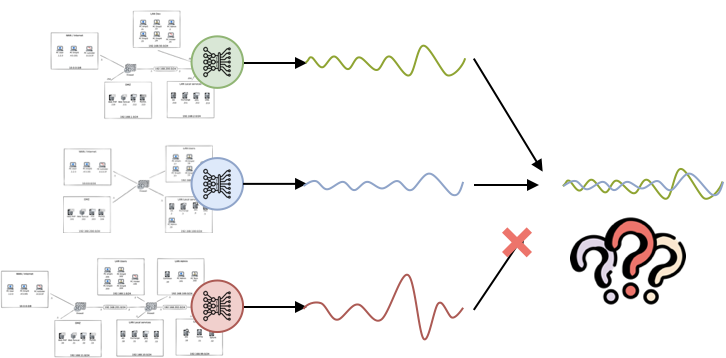
\includegraphics[width=\linewidth]{figures/intro/heterogeneity.png}
        \caption{Heterogeneity headaches.}
      \end{figure}
    \end{column}

    \begin{column}{.5\textwidth}


      \textcolor<2->{lightgray}{%
      \textbf{Challenge I}: \textit{Too much heterogeneity leads to poor performance\dots}~\only<1>{\autocite{lavaur_icdcs_demo_2024}}
      }
      % \only<1>{%
      %   \begin{itemize} \small
      %     \item How to handle different feature sets, data distributions?
      %     \item How to consider models that are dissimilar because they "contain" relevant knowledge?
      %   \end{itemize}
      % }
      \vspace{1ex}


      \textcolor<1,3>{lightgray}{%
      \textbf{Challenge II}: \textit{Difficult to identify malicious contributions when models are different\dots}
      }
      
      % \only<2>{%
      %   \begin{itemize} \small
      %     \item Are model "dissimilar" because they are different, or because they are malicious/poisoned?
      %   \end{itemize}
      % }
      \vspace{1ex}
      
      \only<1-2>{\color{lightgray}}
      \textbf{Challenge III}: \textit{No representative dataset of heterogeneous distributed intrusion detection\dots}~\only<3>{\autocite{lavaur_cesar_2022}}
      
      % \only<3>{%
      % \begin{itemize} \small
      %     \item Datasets are generated locally, lots of different feature sets, no control over heterogeneity.
      %   \end{itemize}
      % }%
    \end{column}
  \end{columns}

  \only<1>{\fcitefootnote{lavaur_icdcs_demo_2024}}
  \only<3>{\fcitefootnote{lavaur_cesar_2022}}
  
\end{frame}


% \begin{frame}{Research Questions}
%   \begin{enumerate}
%     \item What makes applying FL to IDSs specific?
%     \item Can FL be used to federate IDSs across heterogeneous data sources?
%     \item How does FL handle malicious contributions in a federated IDS?
%     \item How can one assess and ensure the trustworthiness of the other participants’ contributions?
%   \end{enumerate}
% \end{frame}


\begin{frame}[b]{Contributions Summary}
  \centering%
  \vspace{-.8cm}
  \foreach \i in {1,...,9} {%
    \includegraphics<\i>[width=1.1\linewidth, center]{./figures/intro/metro/\i.pdf}%
  }
  \includegraphics<10->[width=1.1\linewidth, center]{./figures/intro/metro/10.pdf}%

  \only<11>{
    \tikz[overlay, remember picture,
      shift=(current page.south west),
      x=(current page.south east),
      y=(current page.north west)
    ]{
      % Optional help grid lines
      %\draw[step=.1, opacity=0.3, thick, red] (0,0) grid (1,1);
      
      \node[align=left, anchor=south west] at (.025, .05) {\begin{minipage}{.8\textwidth}
        \tableofcontents
      \end{minipage}};
    }
  }

\end{frame}

% Assessing the Impact of Label-flipping Attacks
% ------------------------------------------------------------------------------

\section{Assessing the Impact of Label-Flipping Attacks}

\begin{frame}
  \sectionpage

  \fcitefootnote{lavaur_ares_bass_2024}
\end{frame}


\begin{frame}{The Problem of Poisoning Attacks}

  \begin{figure}
    \centering
    \foreach \i in {1,...,5}{%
      \includegraphics<\i>[width=.75\textwidth]{figures/assessment/poisoning/\i.pdf}%
    }
    \caption{Poisoning attacks on FL.}
  \end{figure}

\end{frame}

\begin{frame}{Types of Poisoning Attacks}
  \begin{itemize}
    \item By \emph{component}:
    \begin{itemize}
      \item Data poisoning (\eg, \alert<5>{label-flipping}, clean-label attacks, backdoors)
      \item Model poisoning (\eg, gradient boosting, noising)
    \end{itemize}\emph{}

    \pause
    \item By \emph{target}:
    \begin{itemize}
      \item \alert<5>{Untargeted}: affect the model's global performance
      \item \alert<5>{Targeted}: modify its behavior on specific classes or instances
    \end{itemize}

    \pause
    \item By \emph{frequency}:
    \begin{itemize}
      \item one-shot: attacks are performed once
      \item iterative/\alert<5>{continuous}: at each round
      \item adaptive: reacts to the model aggregation
    \end{itemize}

    \pause
    \item By \emph{collusion}:
    \begin{itemize}
      \item \alert<5>{Single attacker}
      \item \alert<5>{Colluding attackers}: multiple coordinated participants
    \end{itemize}
  \end{itemize}
\end{frame}

\begin{frame}{Scope of the Study}
  % \begin{block}{Our work\normalfont~\cite{lavaur_ares_bass_2024}}
  %   Continuous label-flipping attacks in an collaborative intrustion detection context.
  % \end{block}
  \textbf{Existing studies}
  \begin{itemize}
    \item Often partial, focusing on challenging a specific defense mechanism.
    \item Lack of reproducibility and comparability (different datasets, models, and attacks).
    \item No targeted attacks binary classification.
  \end{itemize}

  \pause
  \textbf{Research Questions}
  \begin{enumerate}
    \item Is the behavior of poisoning attacks predictable?
    \item Do hyperparameters influence the impact of poisoning attacks?
    \item Are IDS backdoors realistic using label-flipping attacks?
    \item Is there a critical threshold where label-flipping attacks begin to impact performance?
    \item \alert<3>{Is gradient similarity enough to detect label-flipping attacks?}
  \end{enumerate}
\end{frame}

% \begin{frame}{Experimental Setup}

%   \textbf{Sound experiments}~\cite{uetz_ReproducibleAdaptableLog_2021,ACM_artifacts}:
%   \begin{itemize}
%     \item \emph{valid} (i.e., well-defined and unrefutable);
%     \item \emph{controllable} (e.g., parameterized); and
%     \item \emph{reproducible} (i.e., the same results can be obtained by another group using the author’s artefact).
%   \end{itemize}

% \end{frame}

% \begin{frame}{Experimental Setup}
    
%   Experiment orchestration using \texttt{Eiffel}~\cite{lavaur_icdcs_demo_2024}.
%   \begin{itemize}
%       \item \texttt{Flower} simulation framework~\cite{beutel_Flowerfriendlyfederated_2020} for \gls{fl}.
%       \item \texttt{Hydra} for experiment generation and configuration.
%       \item Custom-made poisoning engine with different attack strategies.
%       \item Nix~\cite{dolstra_purelyfunctionalsoftware_2006} and Poetry to fix system and Python dependencies, enabling reproducibility.
%   \end{itemize}

%   1,067 experiments $\times$ 10 seeds (1,613 hours of computation.)
% \end{frame}


% \begin{frame}{RQ1: Are Poisoning Attacks Predictable?}

%   \begin{figure}
%     \centering
%     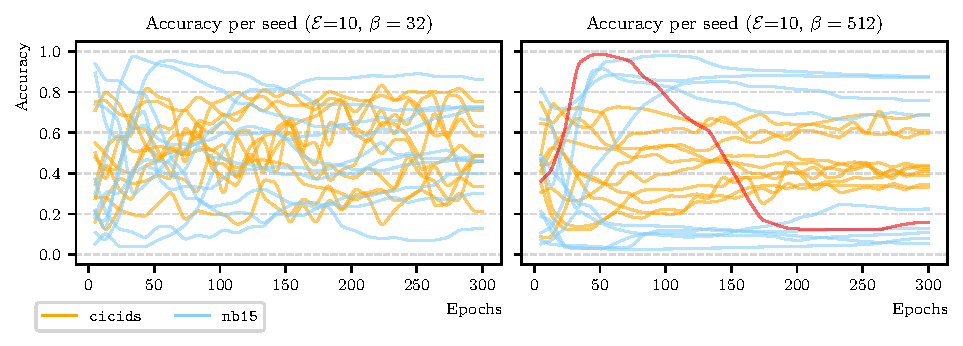
\includegraphics[width=.8\textwidth]{figures/assessment/accuracy_per_seed.pdf}
%     \caption{Predictability of label-flipping attacks.}
%   \end{figure}

%   \begin{itemize}
%     \item Very high variance in the results, but tends to stabilize (on different values) after a few rounds.

%     \item The impact of the attack is highly dependent on the seed.
%     \begin{itemize}
%       \item[$\rightarrow$] Initial parameters, data shuffling, partitioning, \dots
%     \end{itemize}
%   \end{itemize}


% \end{frame}

% \begin{frame}{RQ2: Do Hyperparameters Influence the Impact of Poisoning Attacks?}

%   \begin{figure}
%     \centering
%     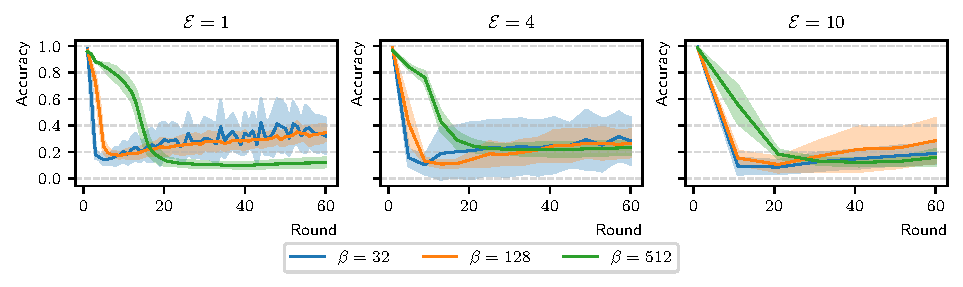
\includegraphics[width=\textwidth]{figures/assessment/hyperparams-late-icdcs.pdf}
%     \caption{Effect of the hyperparameters on the accuracy of the poisoned
%     model in the late scenario (50\% attackers, CICIDS).}
%   \end{figure}

%   \begin{itemize}
%     \item \texttt{late-3} scenario: attackers start poisoning after 3 rounds
%     \item High batch size leads to more inertia, less instantaneous impact
%     \begin{itemize}
%       \item[$\rightarrow$] More impactful in constrained environments
%     \end{itemize}
%   \end{itemize}

% \end{frame}

\begin{frame}{RQ5: Is Gradient Similarity Enough to Detect Label-Flipping Attacks?}

  \begin{columns}
    \begin{column}{.45\textwidth}
      \begin{itemize}
        \item Known technique to detect poisoning attacks~\autocite{tolpegin_DataPoisoningAttacks_2020}.
        \item Higher heterogeneity makes it harder to detect attackers.
        \item Colluding attackers usually form a cluster of their own.
      \end{itemize}
    \end{column}
    \begin{column}{.55\textwidth}
      \begin{figure}
        \centering
        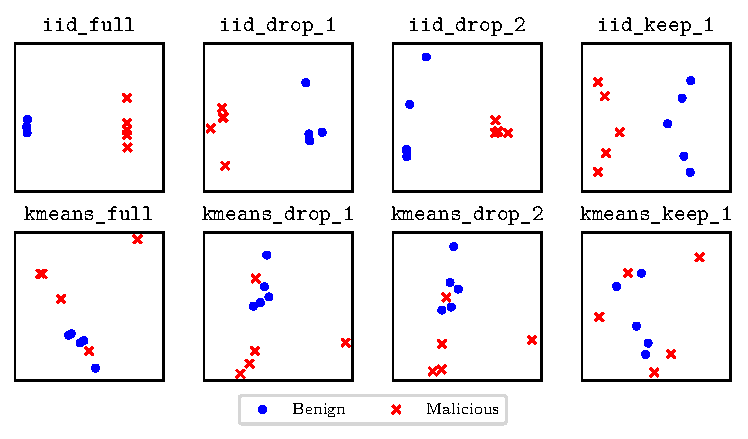
\includegraphics[width=\textwidth]{figures/assessment/similarity-untargeted-colluding-cicids.pdf}
        \caption{PCA projection of the uploaded gradients in 2D (CICIDS).}
      \end{figure}
    \end{column}
  \end{columns}

  \fcitefootnote{tolpegin_DataPoisoningAttacks_2020}

\end{frame}

\begin{frame}{Takeaways}

  A \emph{deeper} understanding of the behavior of label-flipping attacks in FL-based CIDSs.
  \begin{itemize}\small
    \item Unpredictability.
    \item Hyperparameter dependencies, but not on the average performance impact.
    \item Limited by the models' generalization capabilities and the characteristic overlap between classes.
    \item Proximity-based detection techniques show limitations in detecting poisoning attacks.
  \end{itemize}
  
  \onslide<2>{A \alert{reproducible} evaluation framework to study the impact of label-flipping attacks in FIDS
using FL.
  \begin{itemize}\small
    \item Reproducible, extendable, and available in open-access\footnote<2>{https://github.com/leolavaur/eiffel}.
    \item Calls to be extended to other poisoning attacks, datasets, and partitioning strategies.
  \end{itemize}}
\end{frame}

% \begin{frame}{Future Work}

%   \begin{enumerate}    
%     \item Extending the framework
%     \begin{itemize}
%       \item More datasets (currently CICIDS and UNSW-NB15).
%       \item More attack strategies, \eg, backdoors.
%       \item Imrove documentation and usability for other researchers.
%     \end{itemize}

%     \item Deeper heterogeneity study with more realistic assumptions.
%     \begin{itemize}
%       \item Meaningful dataset partitioning.
%       \item Cross-dataset knowledge transfer.
%       \item Leveraging independently generated datasets.
%     \end{itemize}

%   \end{enumerate}

% \end{frame}

% RADAR: Mitigating Byzantine Contributions in Heterogeneous Settings
% ------------------------------------------------------------------------------

\section{Fighting Byzantine Contributions in Heterogeneous Settings}

\begin{frame}
  \sectionpage

  \fcitefootnote{lavaur_radar_2024}
\end{frame}


\begin{frame}{Context}
  % - case study (multiple organizations, partial heterogeneity)
  % - Byzantine contributions -> no guaranties
  \textbf{Case study reminder}
  \begin{itemize}
    \item Multiple organizations collaborating on a federated intrusion detection system.
    \item Partial heterogeneity in the datasets: organizations have different data distributions but can share similarities.
  \end{itemize}

  \textbf{Byzantine contributions}
  \begin{itemize}
    \item No guarantees on the quality of the contributions.
    \item Can be intentional, due to poor data quality, or due to data distribution mismatches.
  \end{itemize}

\end{frame}

\begin{frame}{Problem Statement}
  \begin{block}{Quality Assessment in Heterogeneous Settings}
    For $n$ participants $p_i$ and their local datasets $d_i$ of unknown similarity, each participant uploads a model update $w_i^r$ at each round $r$. Given $P = \{ p_1, p_2, \dots, p_n \} $ and $W = \{ w_1^r, w_2^r, \dots, w_n^r \} $, how can one assess the quality of each participant’s contribution without making assumptions on the data distribution across the datasets $d_i$?
  \end{block}
\end{frame}

\begin{frame}{Existing Solutions}

  \begin{columns}[T]
    
    \begin{column}{.33\textwidth}
      \small\centering
      \textbf{Server-side evaluation}~\autocite{zhou_DifferentiallyPrivateFederated_2022}

      \begin{figure}
        \centering
        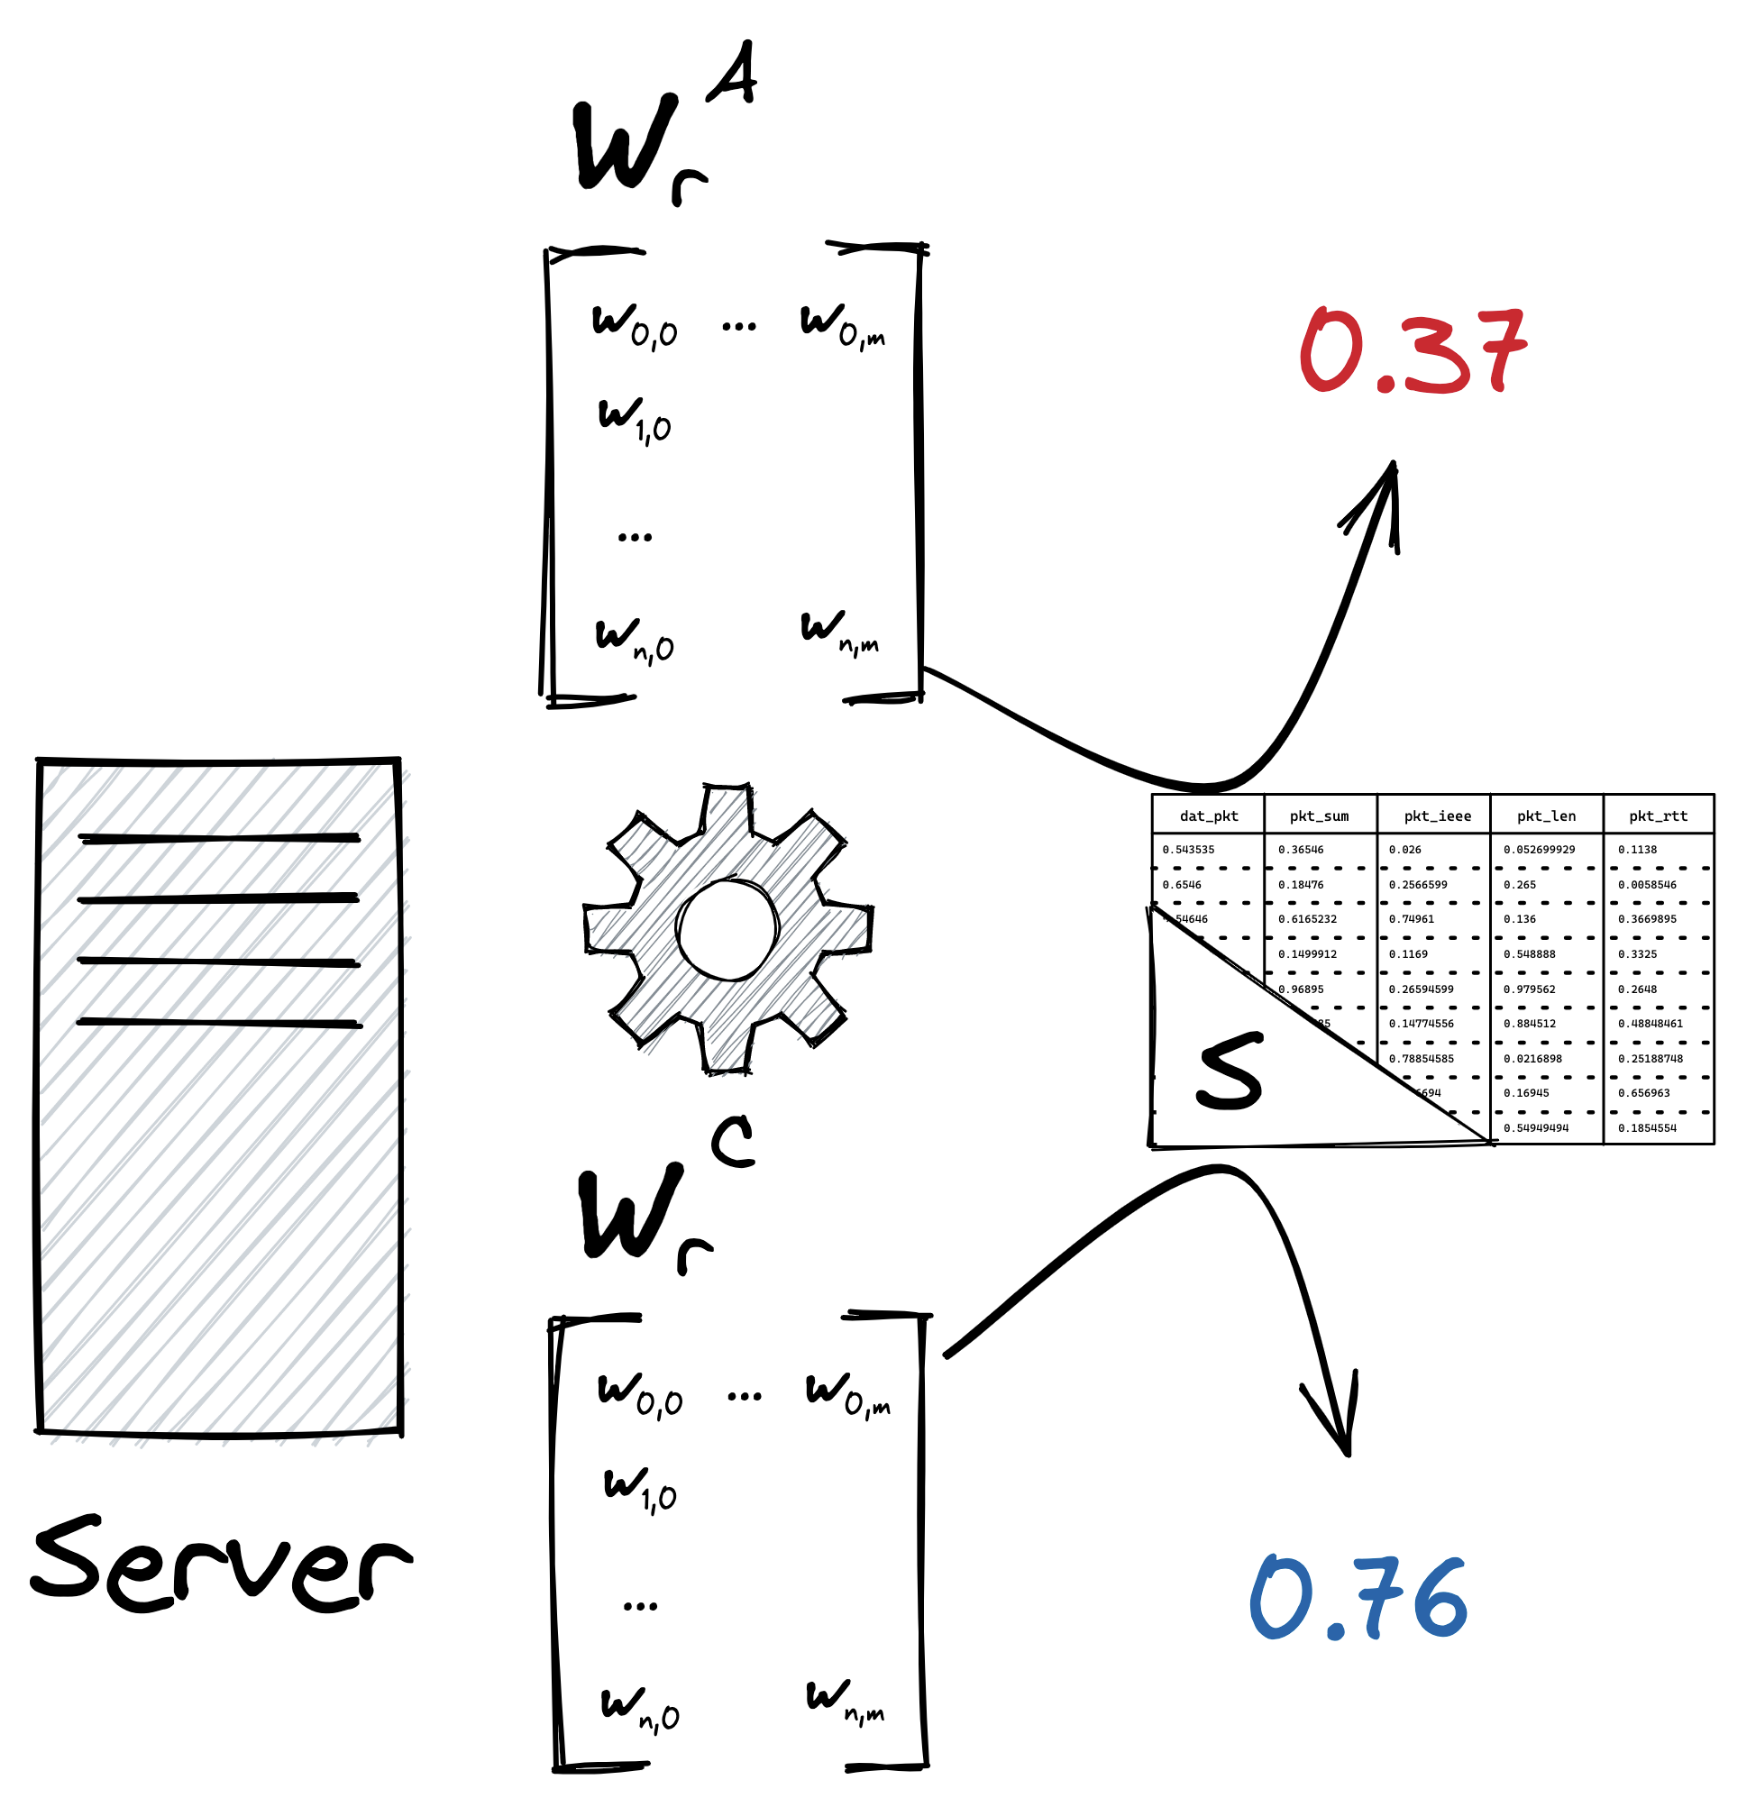
\includegraphics[height=.36\textheight]{figures/radar/server-side-eval}
      \end{figure}

      \begin{itemize}\smaller
        \item Only applicable in IID settings.
        \item Single source of truth.
      \end{itemize}
    \end{column}

    \onslide<2->{%
      \begin{column}{.33\textwidth}
        \small\centering
        \textbf{Server-side comparison}~\autocite{briggs_Federatedlearninghierarchical_2020}

        \begin{figure}
          \centering
          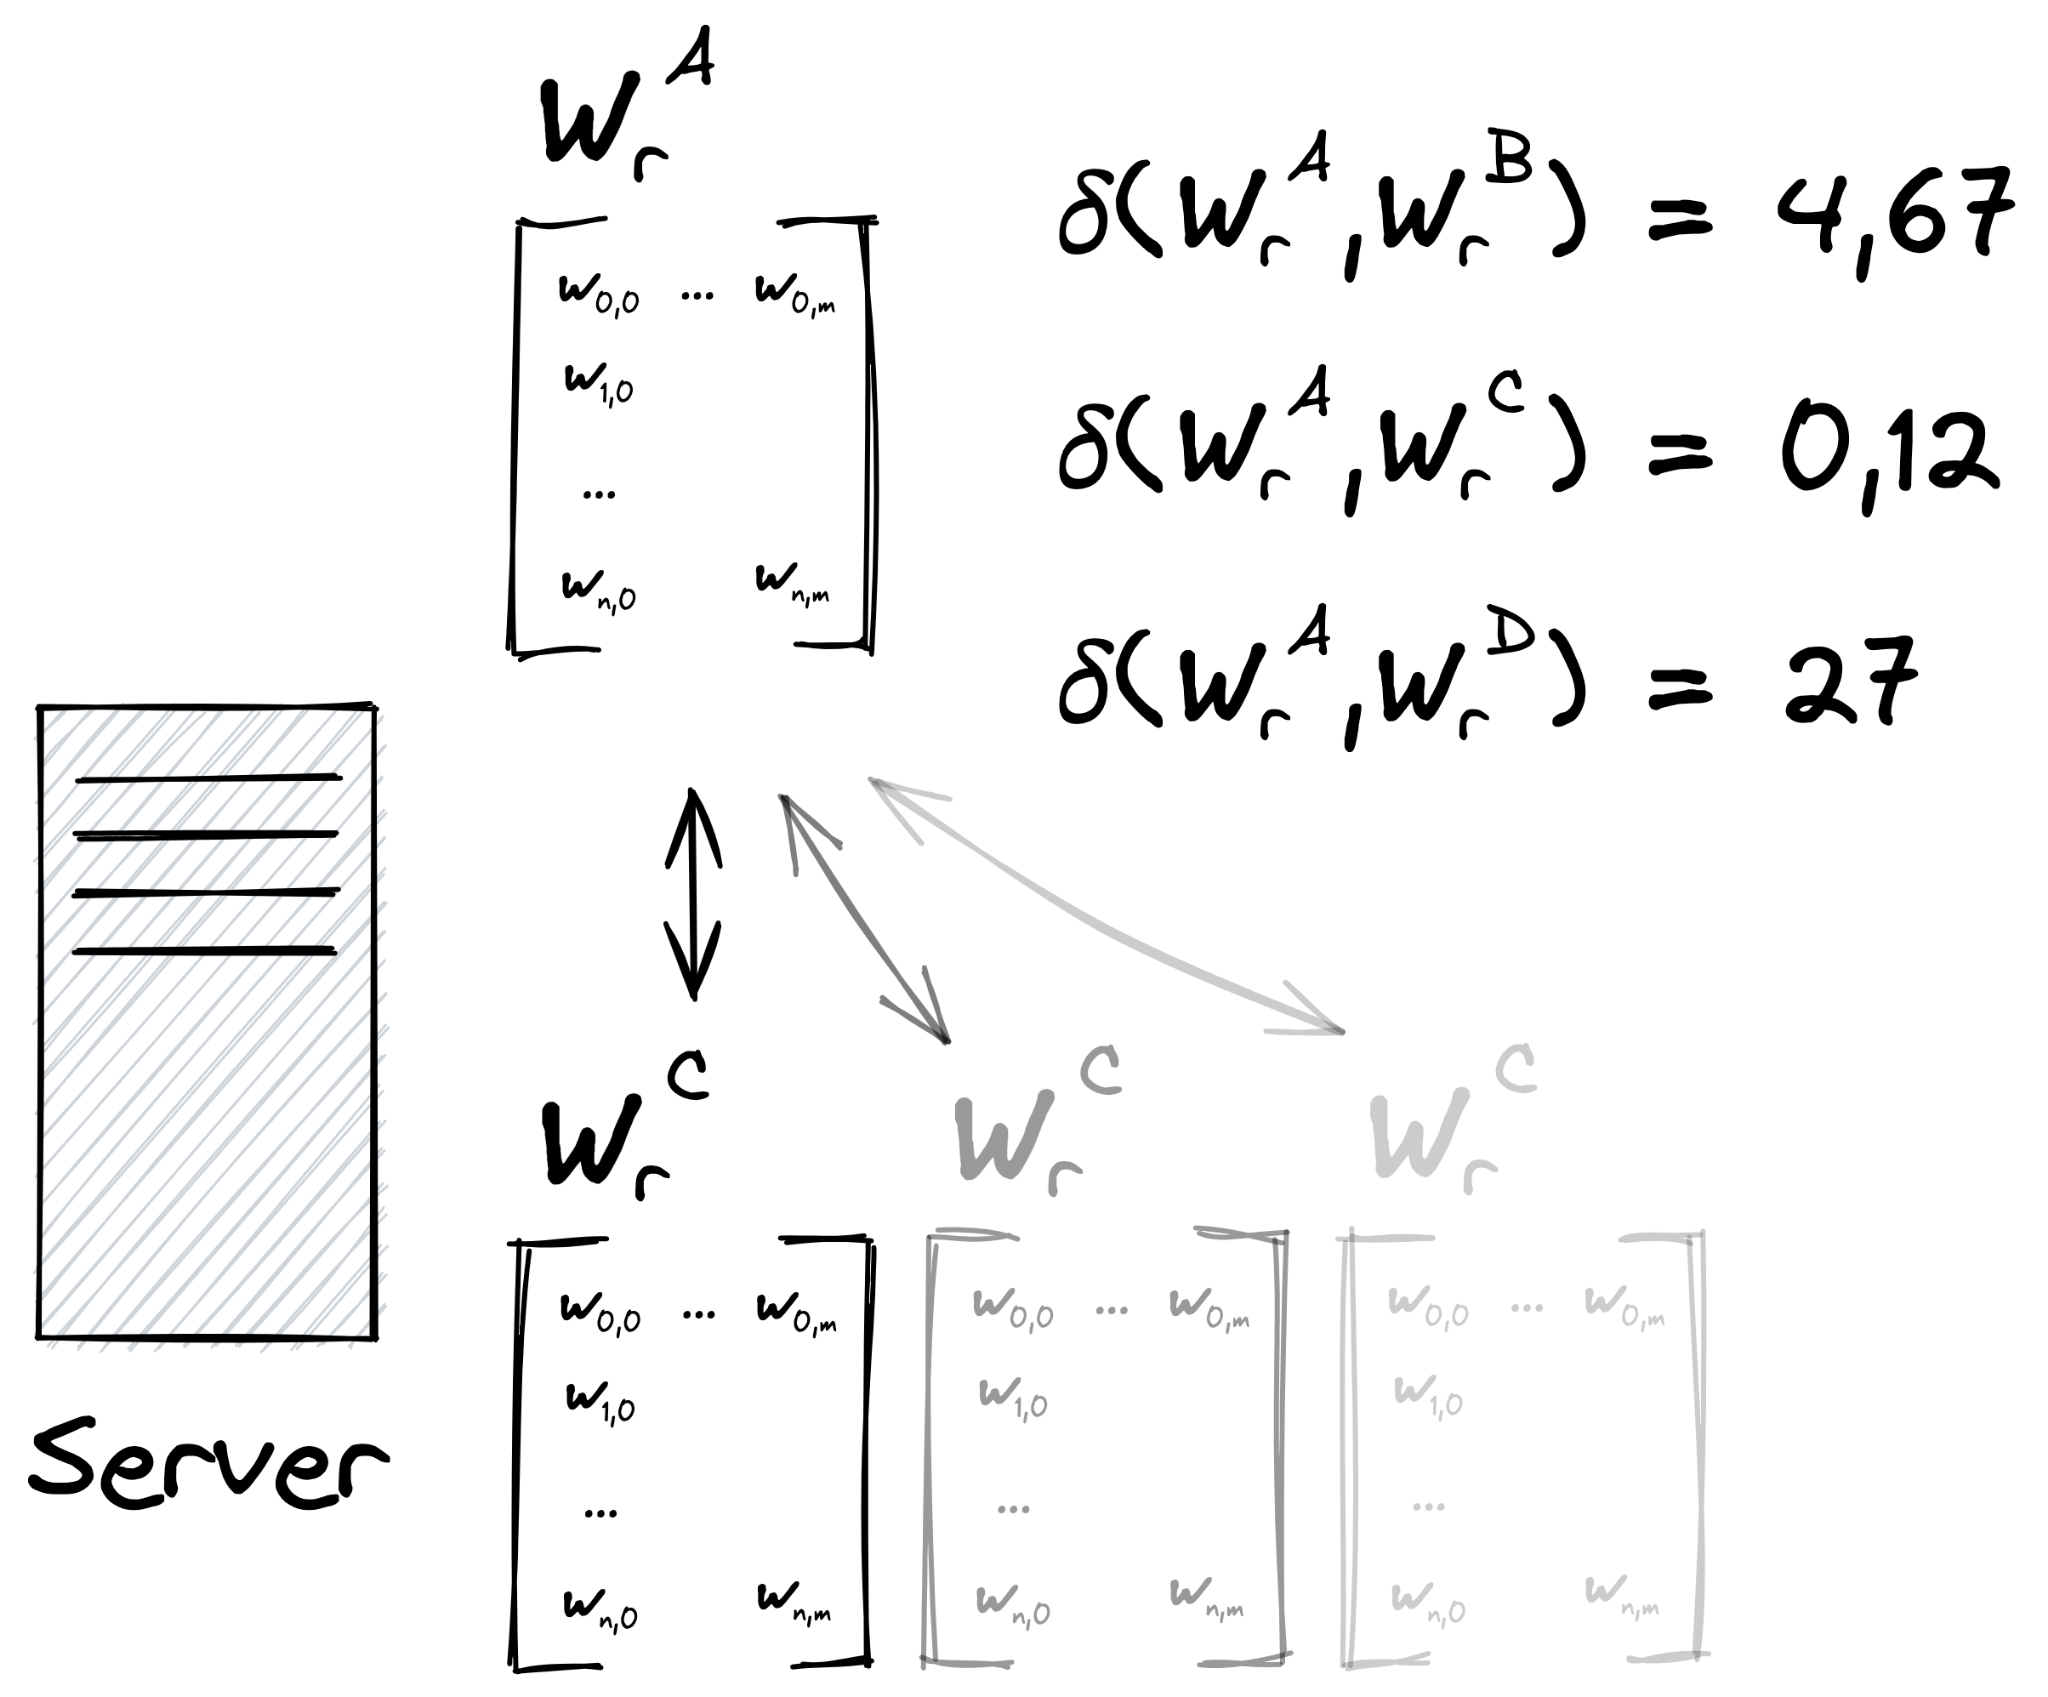
\includegraphics[height=.36\textheight]{figures/radar/server-side-comp}
        \end{figure}

        \begin{itemize}\smaller
          \item Less related to client data.
          \item More appropriate for high-dimensional data.
        \end{itemize}
      \end{column}%
    }

    \onslide<3->{%
      \begin{column}{.33\textwidth}
        \small\centering
        \textbf{Client-side evaluation}~\autocite{zhao_ShieldingCollaborativeLearning_2020}

        \begin{figure}
          \centering
          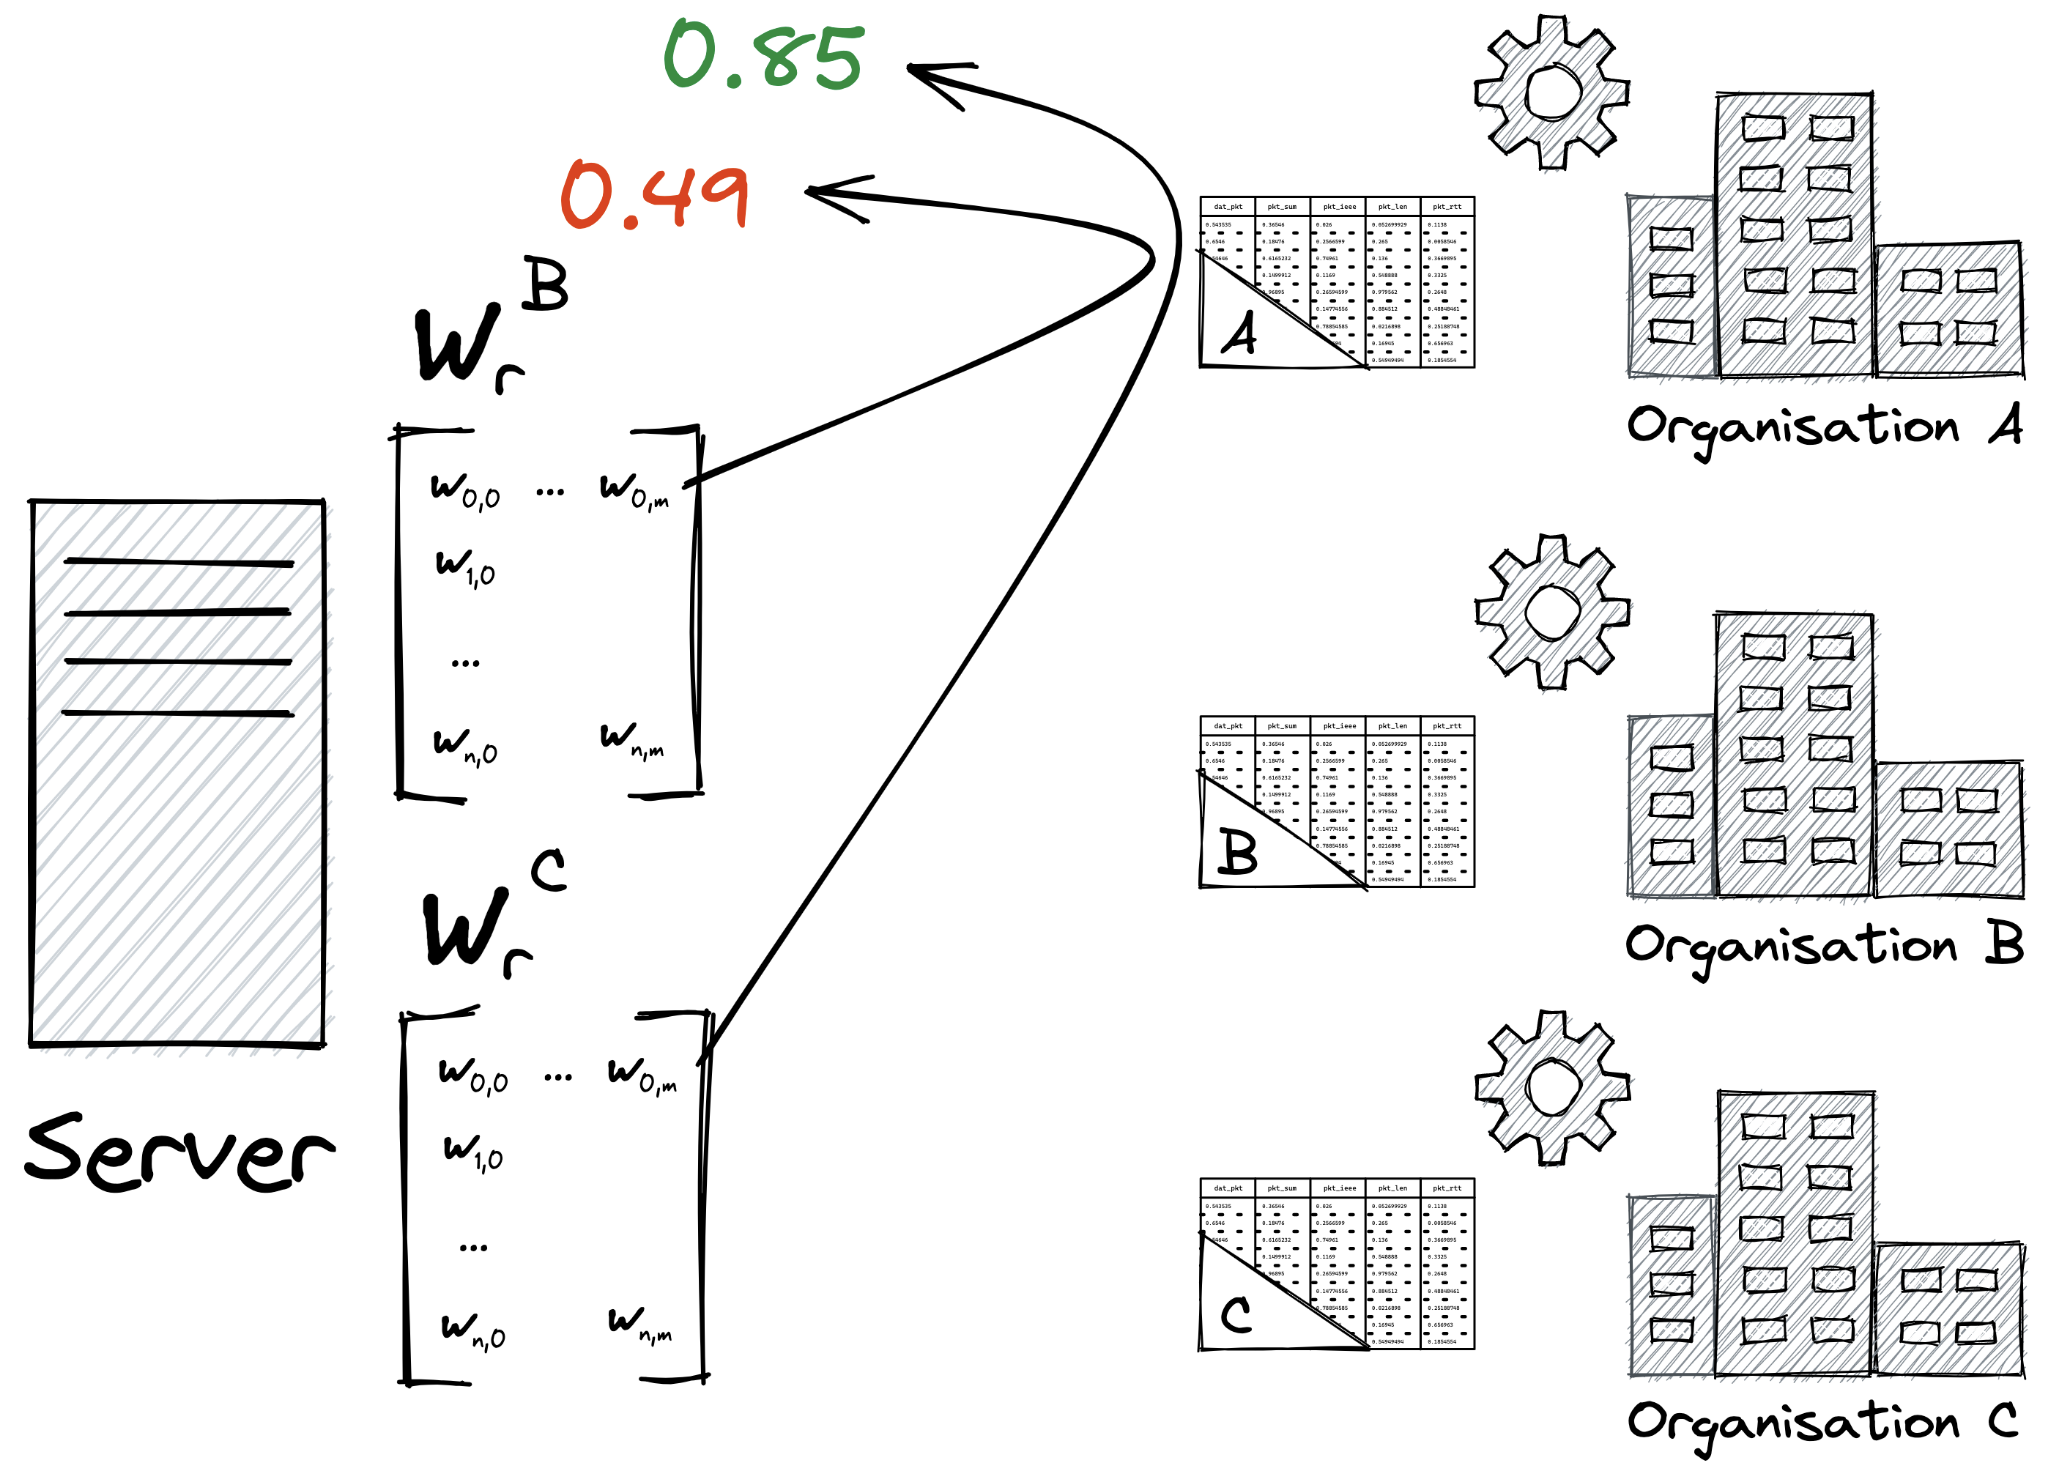
\includegraphics[height=.36\textheight]{figures/radar/client-side-eval}
        \end{figure}

        \begin{itemize}\smaller
          \item High cost in cross-device.
          \item More susceptible to badmouthing.
        \end{itemize}
      \end{column}%
    }

  \end{columns}

  \vspace{3ex}
  
  \fcitefootnote{zhou_DifferentiallyPrivateFederated_2022}
  \only<2->{\fcitefootnote{briggs_Federatedlearninghierarchical_2020}}
  \only<3->{\fcitefootnote{zhao_ShieldingCollaborativeLearning_2020}}

\end{frame}

% \begin{frame}{The RADAR Architecture}

%   \begin{figure}
%     \centering
%     \includegraphics<1>[width=.7\textwidth]{figures/radar/architecture}
%     \includegraphics<2>[width=.7\textwidth]{figures/radar/architecture-xeval}
%     \caption{The RADAR architecture.}
%   \end{figure}


% \end{frame}

\begin{frame}{Assessing Quality with Cross-Evaluation}


  \begin{columns}
    \begin{column}{.45\textwidth}
      \begin{figure}
        \centering
        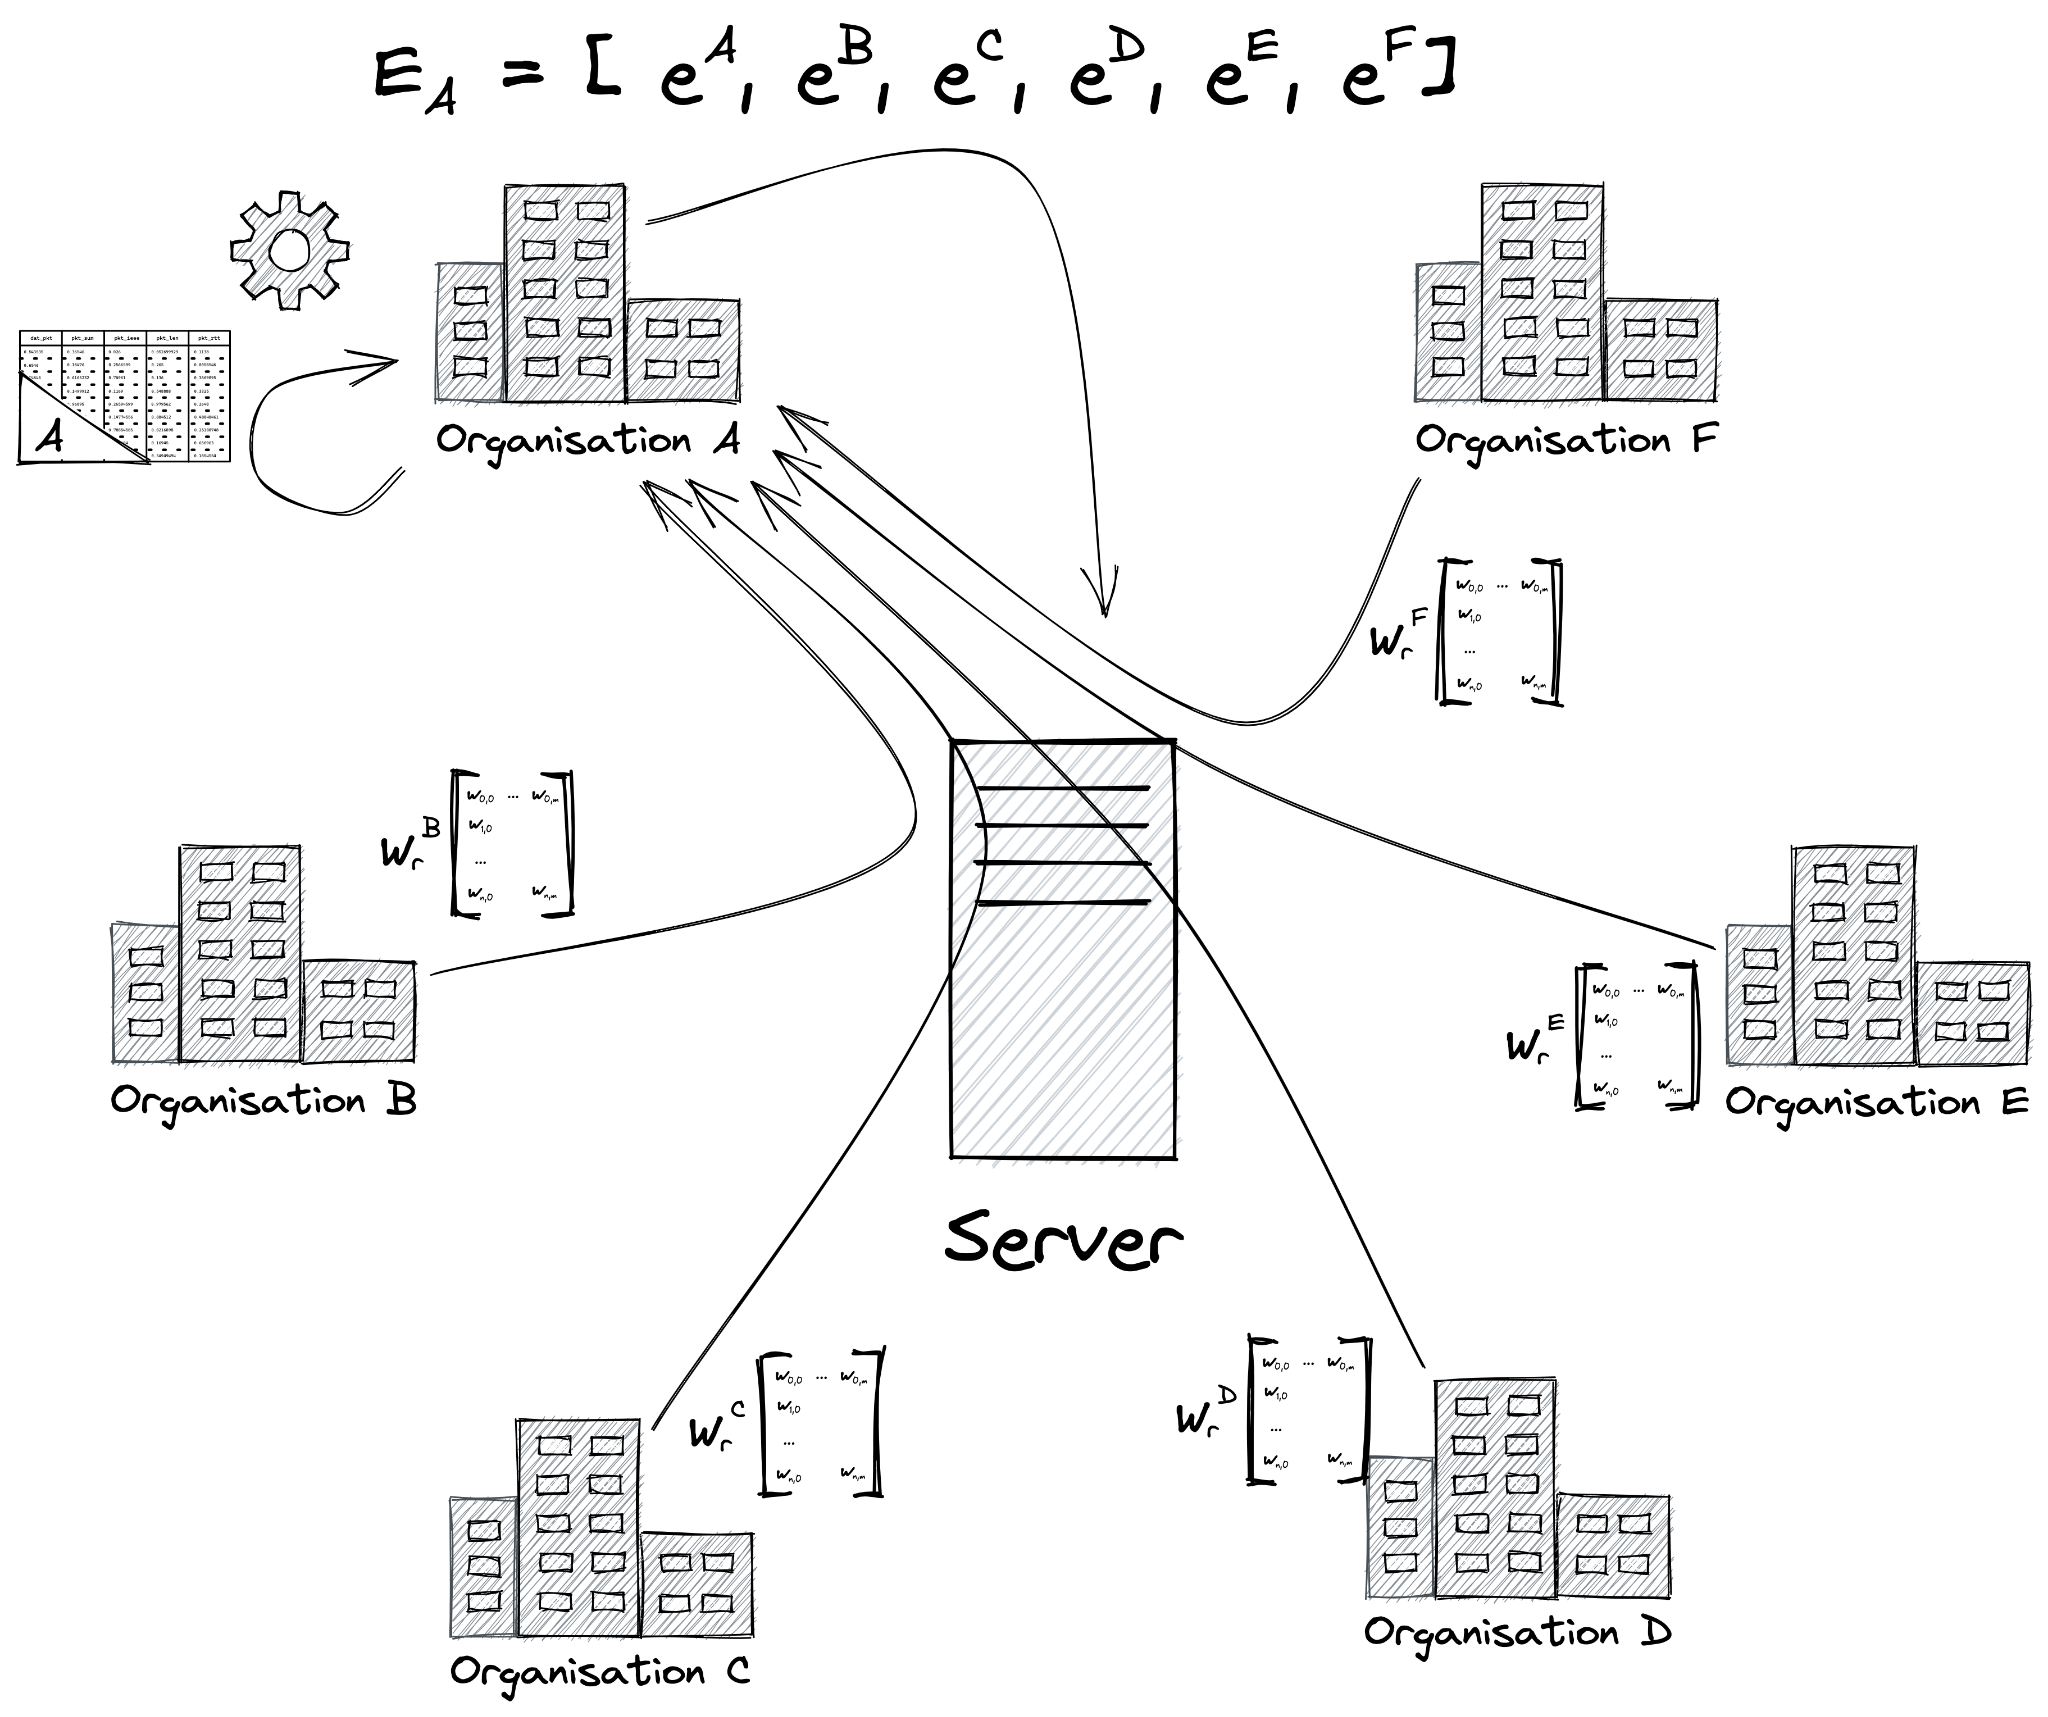
\includegraphics[width=\textwidth]{figures/radar/xeval}
      \end{figure}
    \end{column}
    
    \begin{column}{.55\textwidth}
      \small
      \setlength{\baselineskip}{0.8\baselineskip}
      \vspace{1ex}

      \textbf{Advantages}
      \begin{itemize}
        \item The central server does not need prior knowledge.
        \item Evaluates how each model fits the data (\eg, accuracy, F1 score).
        \item Exhaustive overview of the entire system at each round $r$.
      \end{itemize}

      \onslide<2->{%
        \textbf{Drawbacks}
        \begin{itemize}
          \item High communication and computation costs.
          \item Does not scale well.
          \item Shares local models to participants: less privacy-friendly.
        \end{itemize}
      }

      \onslide<3->{%
        \textbf{But\dots}
        \begin{itemize}
          \item Cross-silo use case: few clients, with reasonable computing capacity.
          \item Slow workflow: long time between rounds.
        \end{itemize}
      }   
    \end{column}

  \end{columns}

\end{frame}


% Parler du thresold dynamique et de sa méthode de calcul. 
% 
\begin{frame}{Fighting Heterogeneity with Clustering}
  
  \textbf{Objective}
  \begin{itemize}
    \item Build \emph{more} homogeneous communities of participants to facilitate model aggregation.
  \end{itemize}


    \pause
    \textbf{Clustering for FL}

    \begin{columns}
        
        \begin{column}{.5\textwidth}
            \begin{itemize}
                \item Distance metric:
                \begin{itemize}
                    \item Between models/gradients;
                    \item L1/L2 Norm, cosine similarity\dots~\cite{briggs_Federatedlearninghierarchical_2020}
                \end{itemize}
            \end{itemize}
        \end{column}
    
        \pause
        \begin{column}{.45\textwidth}
              \begin{itemize}
    
              \item Algorithms:
              \begin{itemize}
                \item Dynamic \emph{split-and-merge}.~\autocite{chen_ZeroKnowledgeClustering_2021}
                \item Hierarchical clustering.~\autocite{briggs_Federatedlearninghierarchical_2020}
              \end{itemize}
            \end{itemize}
    
        \end{column}
    \end{columns}

    \only<2->{\fcitefootnote{briggs_Federatedlearninghierarchical_2020}}
    \only<3->{\fcitefootnote{chen_ZeroKnowledgeClustering_2021}}
\end{frame}

\begin{frame}{Fighting Heterogeneity with Clustering}
    \begin{columns}
        \begin{column}{.4\textwidth}

        Leverage cross-evaluation results instead of model updates:
        \begin{itemize}
            \item subjective similarity estimation;
            \item similar evaluations $\rightarrow$ similar data distributions;
        \end{itemize}

        \end{column}
        \begin{column}{.6\textwidth}
            \begin{figure}
                \centering
                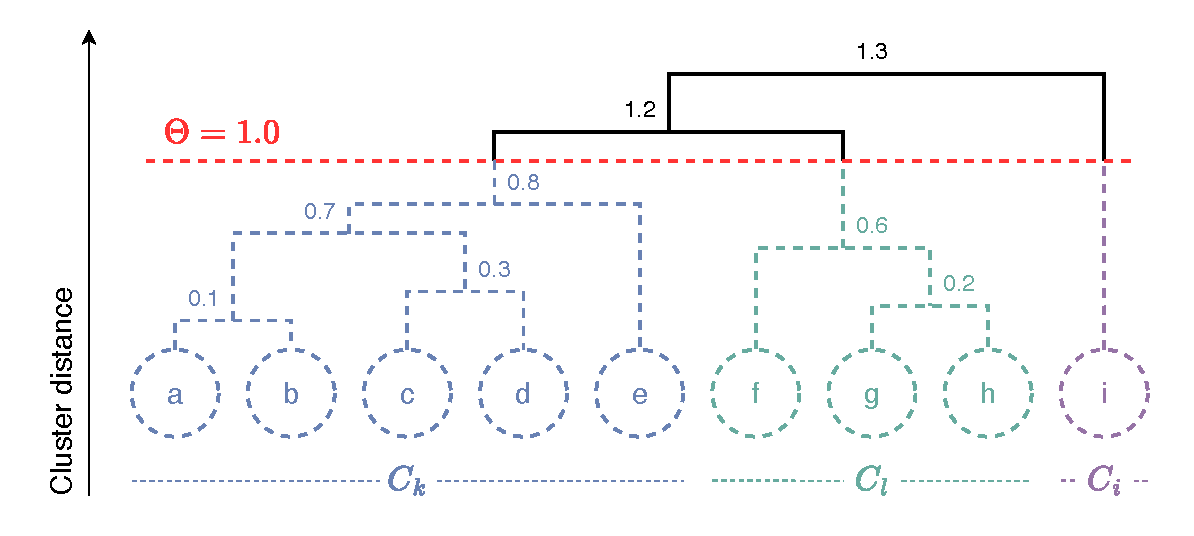
\includegraphics[width=\textwidth]{figures/radar/clustering.drawio.pdf}
                % \makebox[\textwidth][c]{%
                %   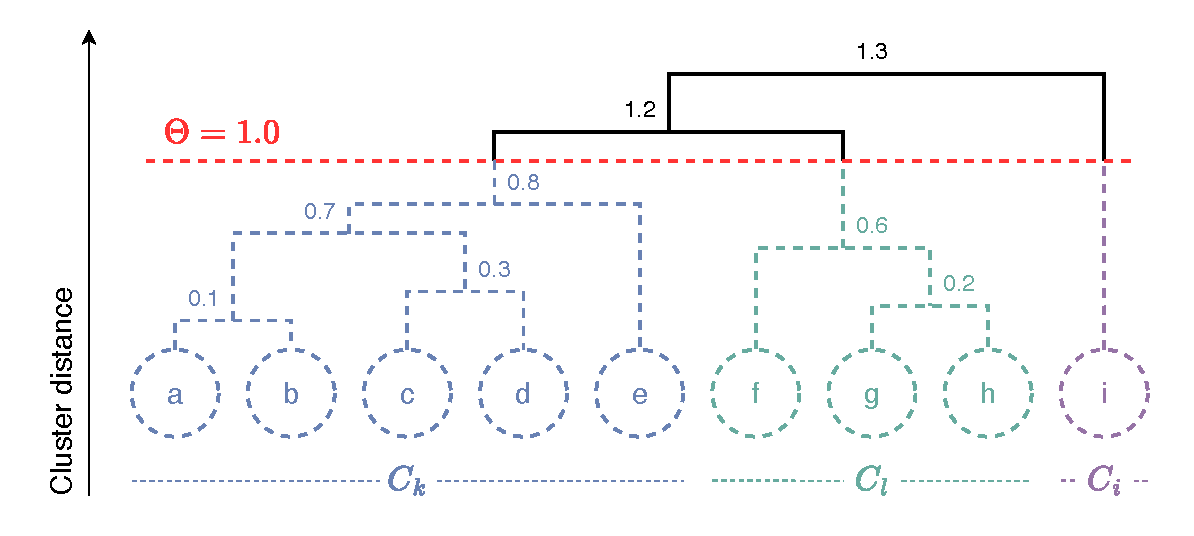
\includegraphics[width=1.2\textwidth]{figures/radar/clustering.drawio.pdf}%
                % }
                \caption{Hierarchical clustering.}
            \end{figure}
        \end{column}
    \end{columns}
\end{frame}


\begin{frame}{Reputation-aware Aggregation}

  \begin{block}{Definition: Reputation Systems\normalfont~\autocite{resnick_Reputationsystems_2000}}
    \begin{itemize}
      \item Long-lived entities that inspire an expectation of future interaction;
      \item Capture and distribution of feedback about current interactions (such information must be visible in the future); and
      \item Use of feedback to guide trust decisions.
    \end{itemize}
  \end{block}

  \onslide<2>{%
    \begin{itemize}
      \item Dirichlet distribution for local aggregation of the reputation scores.~\autocite{fung_DirichletBasedTrustManagement_2011}
      \item Votes weighted by the similarity inside each cluster.
      \item Exponential decay for potential redemption.
    \end{itemize}
  }

  \fcitefootnote{resnick_Reputationsystems_2000}
  \only<2>{%
    \fcitefootnote{fung_DirichletBasedTrustManagement_2011}
  }

\end{frame}

\begin{frame}{Experimental Setup}
  \begin{columns}
    \begin{column}{.55\textwidth}
      Similar setup as in the previous case study:
      \begin{itemize}
        \item Heterogeneous datasets, but some participants can share similarities.
        \item 4 datasets: CIC-CSE-IDS2018, UNSW-NB15, Bot-IoT, ToN\_IoT.
        \item NF-V2~\autocite{sarhan_StandardFeatureSet_2021} feature set (\ie, NetFlow V9).
      \end{itemize}
    \end{column}
    \begin{column}{.45\textwidth}
      \begin{figure}

        \includegraphics<1>[height=.5\textheight,left]{figures/radar/distribution.png}%
        \includegraphics<2>[height=.5\textheight,left]{figures/radar/distribution-attack.png}%

        \caption{Distribution of the datasets.}
      \end{figure}
    \end{column}
  \end{columns}
  \fcitefootnote{sarhan_StandardFeatureSet_2021}
\end{frame}

\begin{frame}{Results}
  \begin{table}
    \centering
    \caption{
      \emph{Effect of different attack configurations (untargeted) on all baselines.}
      \texttt{RA} is RADAR, \texttt{FG} is \texttt{FoolsGold}, \texttt{FA} is \texttt{FedAvg} (on \emph{all} participants), and \texttt{FC} is \texttt{FedAvg} ideally clustered per dataset.
    }

    \footnotesize

    \newcommand{\hl}{}
    \only<2>{\renewcommand{\hl}{\cellcolor{imta-green!30}}}


  
    \setlength\tabcolsep{1ex}
    \begin{tabularx}{.5\textwidth}{lX|rrrr}
      \toprule % ---------------------------------
      \multicolumn{2}{c|}{\multirow{2}{*}{\textbf{Scenario}}} & \multicolumn{4}{c}{\textbf{\gls{asr}} (\%)} \\
      & & \multicolumn{1}{c}{\texttt{RA}} & \multicolumn{1}{c}{\texttt{FG}} & \multicolumn{1}{c}{\texttt{FA}} & \multicolumn{1}{c}{\texttt{FC}} \\
      \midrule % ---------------------------------
      % TARGETED ATTACKS
      \multicolumn{2}{l|}{\textbf{Targeted} (\texttt{100T})} & & & & \\
                  & \texttt{Benign}       &  \hl \textbf{0.00} &  5.17 & 5.10 &  0.09 \\
                  & \texttt{Lone}         &  \hl \textbf{0.00} & 93.82 & 6.73 &  0.45 \\
                  & \texttt{Collud. min.} &  \hl \textbf{0.00} &  2.97 & 9.99 & 53.40 \\
                  & \only<3>{\cellcolor{red!20}} \texttt{Collud. maj.} &  \only<3>{\cellcolor{red!20}} 73.39 & \textbf{8.10} & 17.65 & 59.36 \\
      \midrule % ---------------------------------
      % UNTARGETED ATTACKS
      \multicolumn{2}{l|}{\textbf{Untargeted} (\texttt{100U})} & & & & \\
      & \texttt{Benign}        & \hl 0.09  & 0.39 & 33.30 & \textbf{0.06} \\
      & \texttt{Lone}          & \hl \textbf{0.08} & 99.89 & 54.70 & 0.12 \\
      & \texttt{Collud. min.}  & \hl 0.10 & \textbf{0.04} & 44.53 & 6.26 \\
      & \texttt{Collud. maj.}  & \hl \textbf{0.08} & 38.98 & 59.49 & 94.36 \\          
      \bottomrule % ---------------------------------
      \small & \multicolumn{1}{c}{} & \multicolumn{4}{c}{\emph{lower is better}}
    \end{tabularx}
  \end{table}
  
\end{frame}

% \begin{frame}{Results}
%   \begin{figure}
%     \centering
%     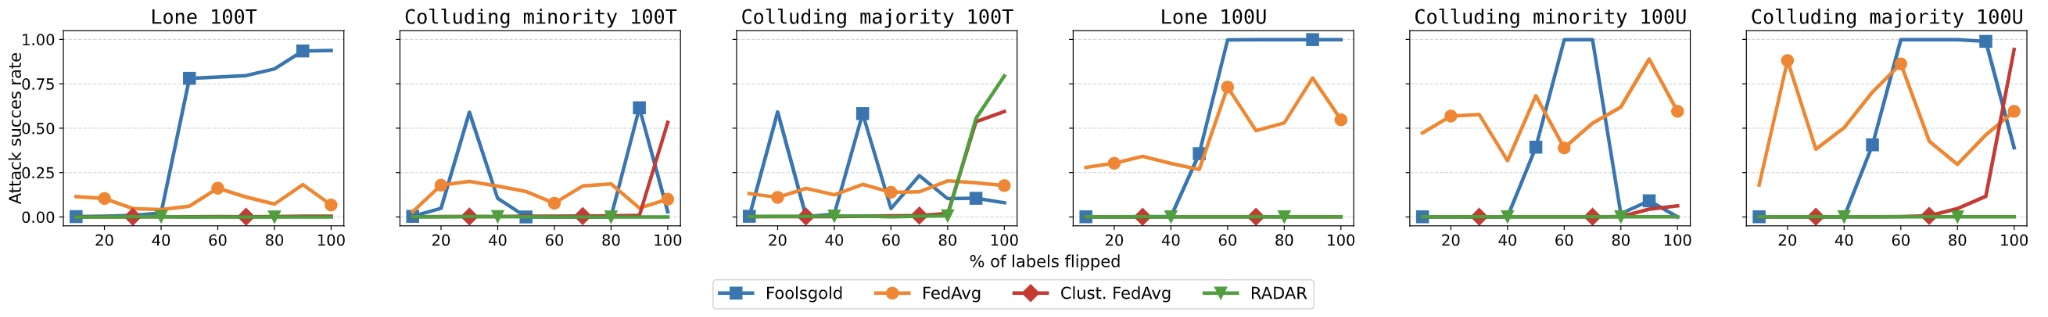
\includegraphics[width=.9\textwidth]{figures/radar/baselines.png}
%     \caption{Baseline comparison.}
%   \end{figure}
%   \begin{figure}
%     \centering
%     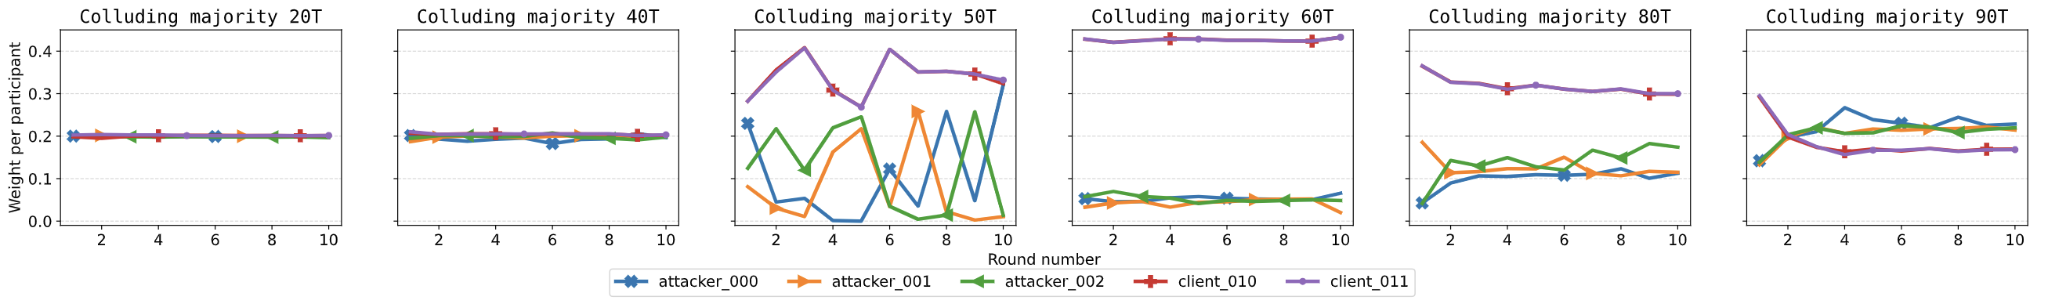
\includegraphics[width=.9\textwidth]{figures/radar/limiting-case.png}
%     \caption{RADAR's limiting scenario.}
%   \end{figure}
% \end{frame}

\begin{frame}{Takeaways}
  \textbf{The proposed framework can:}
  \begin{itemize}
    \item Accurately cluster similar participants based on cross evaluations results.
    \item Mitigate label-flipping untargeted attacks via clustering.
    \item Mitigate most label-flipping targeted attacks, including colluding attackers (up to 80\% of poisoned data).
  \end{itemize}

  \onslide<2>{%
    \textbf{Future works:}
    \begin{itemize}
      \item Remove the central server dependency.
      \item Reduce the cross-evaluation overhead to extend applicability to cross device settings.
      \item Test the approach in more realistic heterogeneous settings.
    \end{itemize}
  }
\end{frame}


% Conclusion
% ------------------------------------------------------------------------------

\section*{Conclusion}

\begin{frame}
  \sectionpage
\end{frame}

\begin{frame}{Contributions}
  \centering
  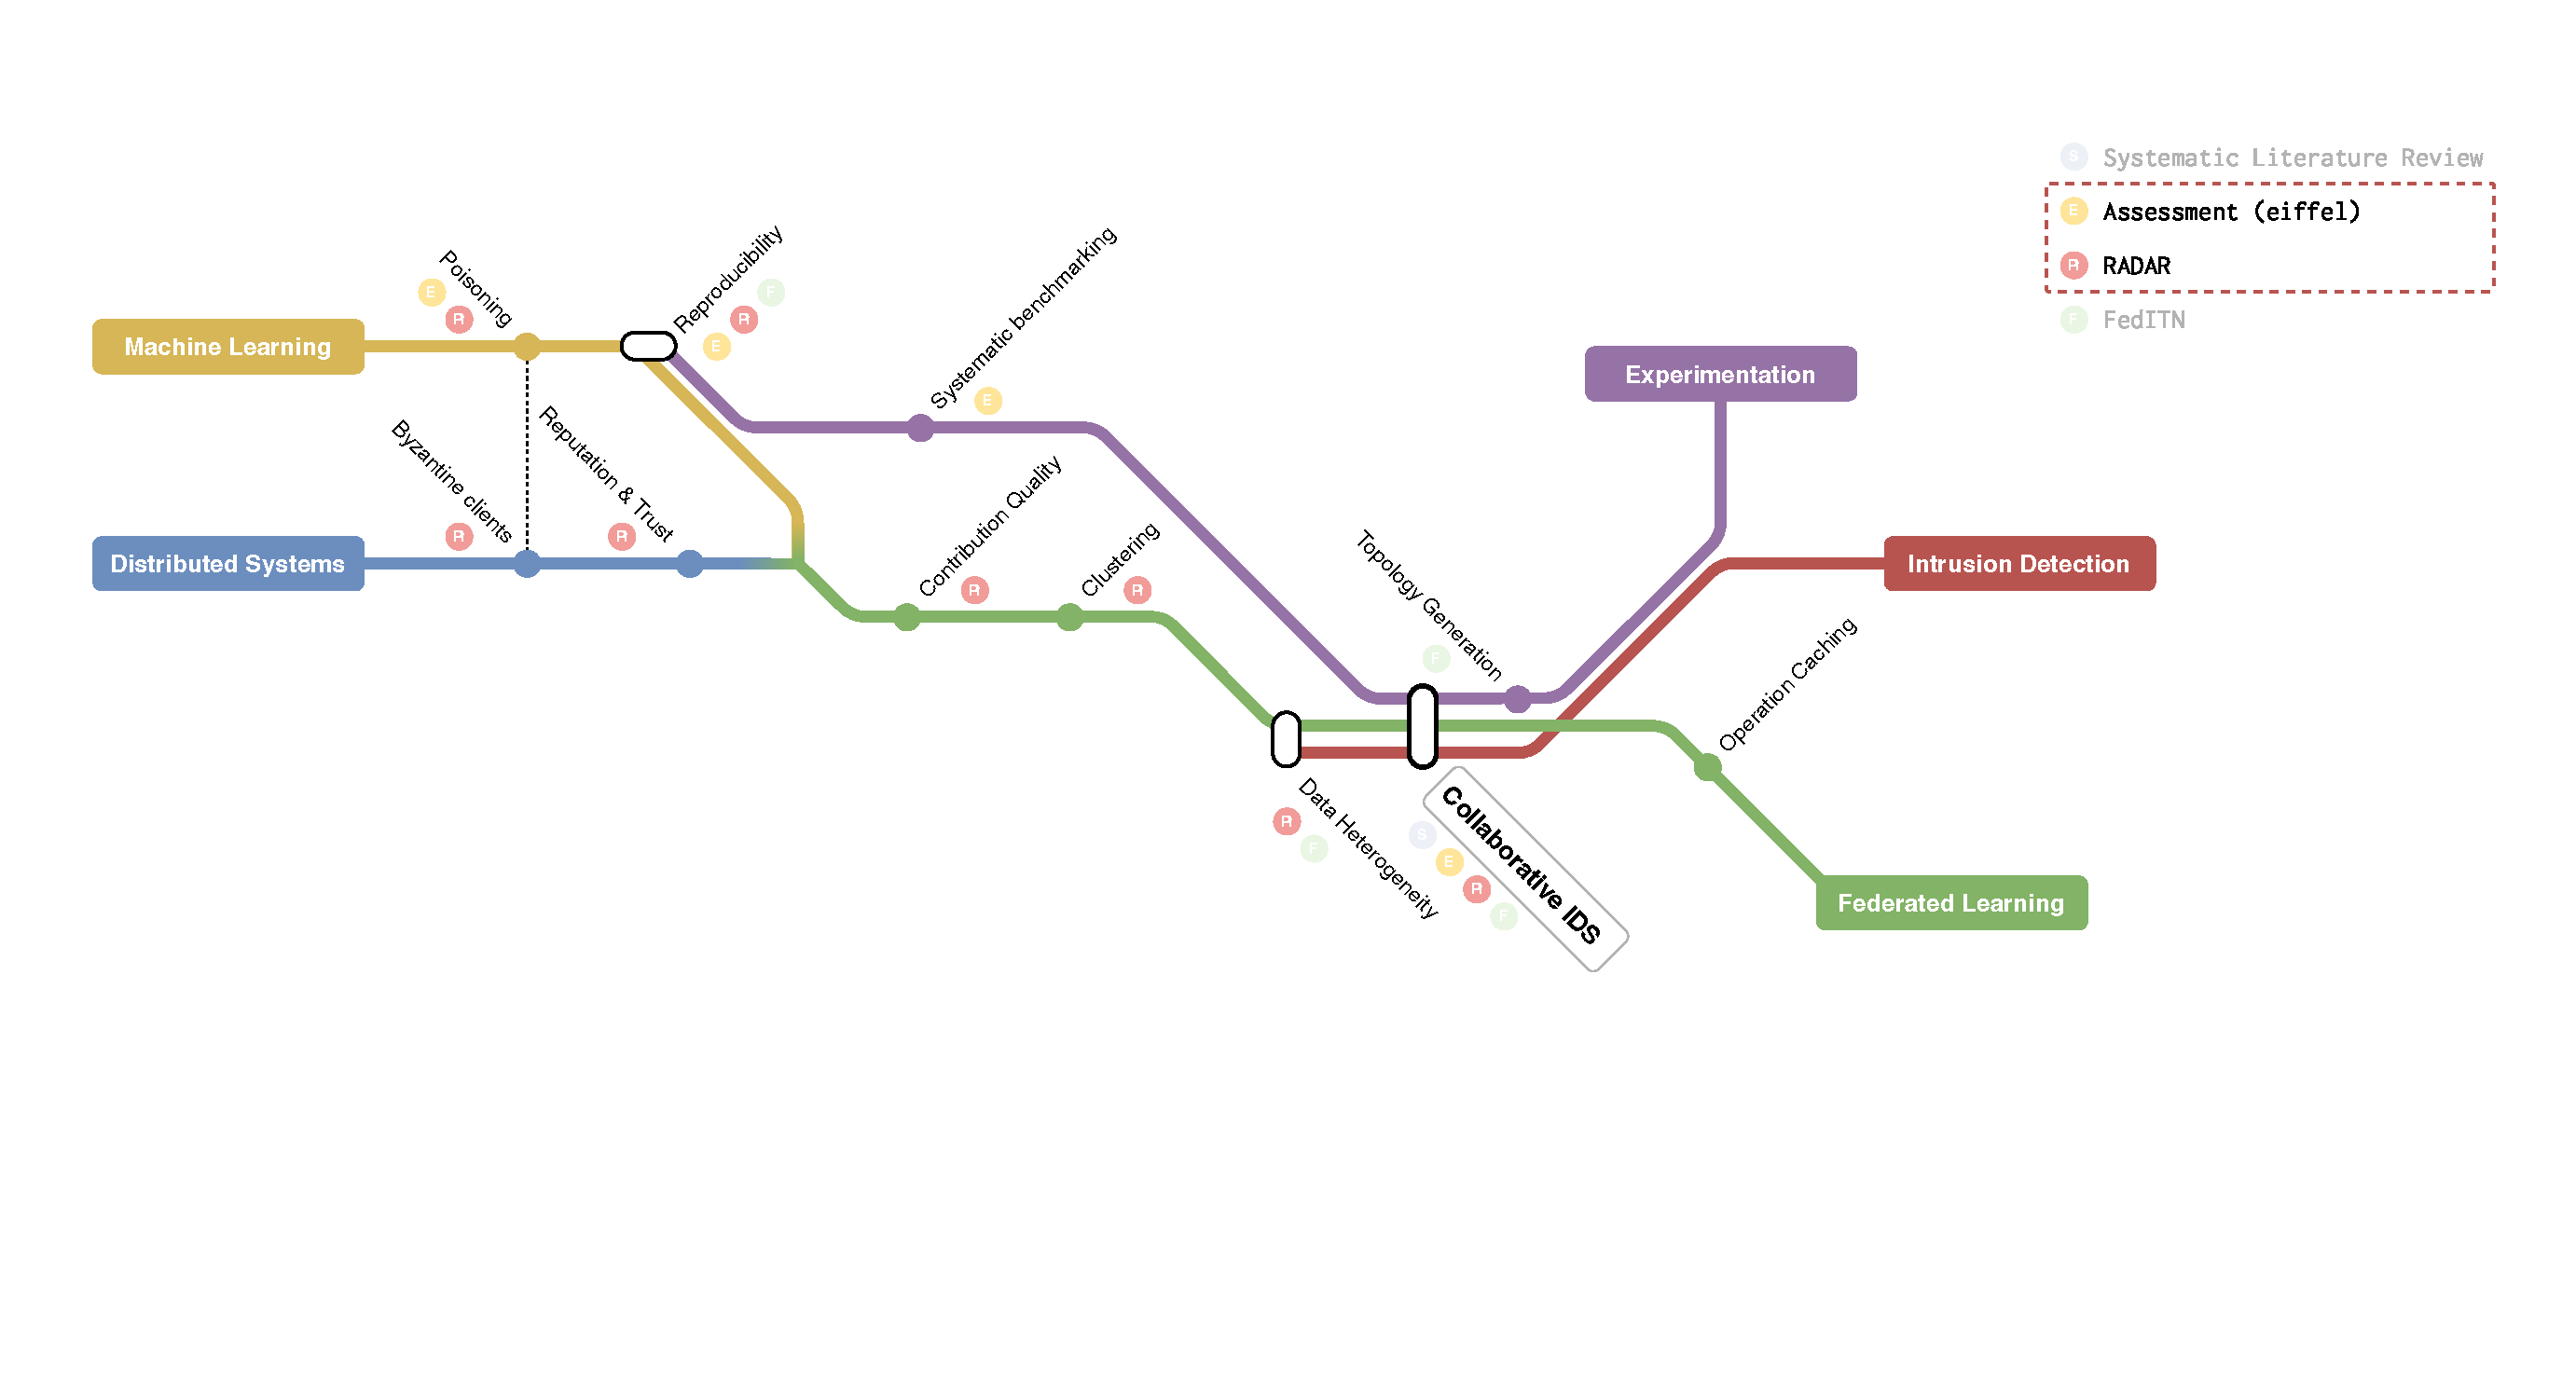
\includegraphics[width=1.1\textwidth, center]{figures/intro/metro/12.pdf}%
  
\end{frame}

% \begin{frame}{Contributions}
%   \textbf{Federated IDSs}
%   \begin{itemize}
%     \item SLR on FIDSs to structure the research field~\autocite{lavaur_tnsm_2022,lavaur_cesar_2022}, with a demonstration of their potential and limitations~\autocite{lavaur_icdcs_demo_2024}
%     \item Assessment of the impact of label-flipping attacks on FIDSs~\autocite{lavaur_ares_bass_2024}, enabled by a reproducible experimental framework
%     \item Countermeasure against Byzantine contributors in FIDSs~\autocite{lavaur_radar_2024}
%   \end{itemize}

%   \onslide<2->{%
%     \textbf{Generating datasets} (the FedITN project)
%     \begin{itemize}
%       \item Constraint-based generation of realistic network topologies (not published yet)
%       \item Generation of realistic network traffic datasets (ongoing work)
%     \end{itemize}
%   }

%   \onslide<3->{%
%     \textbf{Federated Learning}
%     \begin{itemize}
%       \item Feasibility study of operation-caching in FL using Information Centric Networking (ICN)
%       \begin{itemize}
%         \item[$\rightarrow$] Work of Gabriel Bourgeois as part of his Master's internship.
%       \end{itemize}
%     \end{itemize}
%   }
% \end{frame}


% \begin{frame}{Perspectives}
%   \textbf{Four research axes to go beyond FIDSs}
%   \begin{enumerate}
%     \item Modern Detection Techniques
%       \begin{itemize}
%         \item Better representation (\eg, knowledge graphs, embedding, \alert<2>{causality modeling}), explainability, and handling \alert<2>{partial observability}.
%       \end{itemize}
    
%     \item Federated Learning and Derivatives
%       \begin{itemize}
%         \item Handling heterogeneity, trust, decentralization, and going beyond the application layer.
%       \end{itemize}

%     \item Evaluation
%       \begin{itemize}
%         \item More realistic datasets, apt methodologies, and reproducibility.
%       \end{itemize}

%     \item Integration in the Regulatory Landscape
%       \begin{itemize}
%         \item Privacy, data protection, fairness, and compliance with regulations.
%       \end{itemize}

%   \end{enumerate}

% \end{frame}

\begin{frame}[b]{Future Work}
  \centering%
  \foreach \i in {1,...,4} {%
    \includegraphics<\i>[width=1.1\textwidth, center]{figures/conclusion/future/\i.pdf}%
  }%
\end{frame}


\begin{frame}[b]{Going beyond FIDSs}
  \centering
  \foreach \i in {1,...,9} {%
    \includegraphics<\i>[width=1.1\textwidth, center]{figures/conclusion/perspectives/\i.pdf}%
  }%
\end{frame}


\begin{frame}
  \centering
  \scshape\Large Thank you for your attention!

  \vfill
  
  \normalshape\normalsize

  \textbf{Improving Intrusion Detection in Distributed Systems with Federated Learning}
  
  \bigskip
  \raggedright
  \begin{itemize}
    \item Three publications in international \alert{conferences}: ICDCS 2024, ARES (BASS) 2023, and SRDS 2024.
    \item One article in an international \alert{journal}: IEEE TNSM.
    \item National and international \alert{tutorials} on Federated Learning for Intrusion Detection: EUR CyberSchool's Spring Research School 2023, NoF 2023 and ICDCS 2024.
  \end{itemize}

  \vfill
\end{frame}
%
\appendix

\begin{frame}[allowframebreaks]{References}
  \printbibliography[heading=none]
\end{frame}

\section*{Extra Slides: Assessment}

\begin{frame}
  \sectionpage
\end{frame}

\begin{frame}{Experimental Setup}

  \textbf{Sound experiments}~\cite{uetz_ReproducibleAdaptableLog_2021,ACM_artifacts}:
  \begin{itemize}
    \item \emph{valid} (i.e., well-defined and unrefutable);
    \item \emph{controllable} (e.g., parameterized); and
    \item \emph{reproducible} (i.e., the same results can be obtained by another group using the author’s artefact).
  \end{itemize}

\end{frame}

\begin{frame}{Experimental Setup}
    
  Experiment orchestration using \texttt{Eiffel}~\cite{lavaur_icdcs_demo_2024}.
  \begin{itemize}
      \item \texttt{Flower} simulation framework~\cite{beutel_Flowerfriendlyfederated_2020} for \gls{fl}.
      \item \texttt{Hydra} for experiment generation and configuration.
      \item Custom-made poisoning engine with different attack strategies.
      \item Nix~\cite{dolstra_purelyfunctionalsoftware_2006} and Poetry to fix system and Python dependencies, enabling reproducibility.
  \end{itemize}

  1,067 experiments $\times$ 10 seeds (1,613 hours of computation.)
\end{frame}


\begin{frame}{RQ1: Are Poisoning Attacks Predictable?}

  \begin{figure}
    \centering
    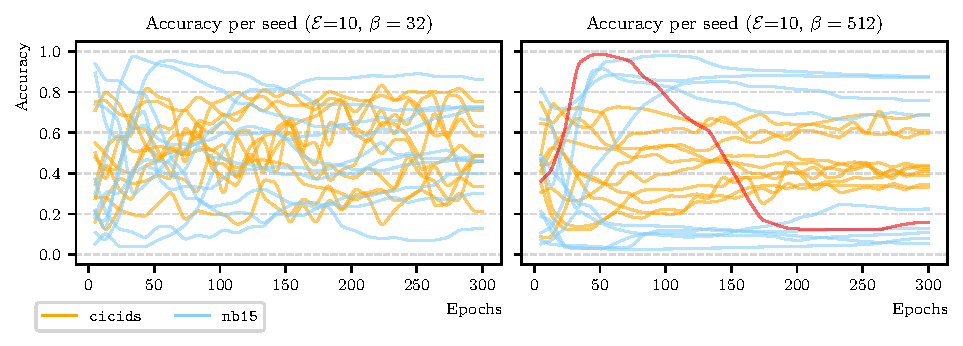
\includegraphics[width=.8\textwidth]{figures/assessment/accuracy_per_seed.pdf}
    \caption{Predictability of label-flipping attacks.}
  \end{figure}

  \begin{itemize}
    \item Very high variance in the results, but tends to stabilize (on different values) after a few rounds.

    \item The impact of the attack is highly dependent on the seed.
    \begin{itemize}
      \item[$\rightarrow$] Initial parameters, data shuffling, partitioning, \dots
    \end{itemize}
  \end{itemize}


\end{frame}

\begin{frame}{RQ2: Do Hyperparameters Influence the Impact of Poisoning Attacks?}

  \begin{figure}
    \centering
    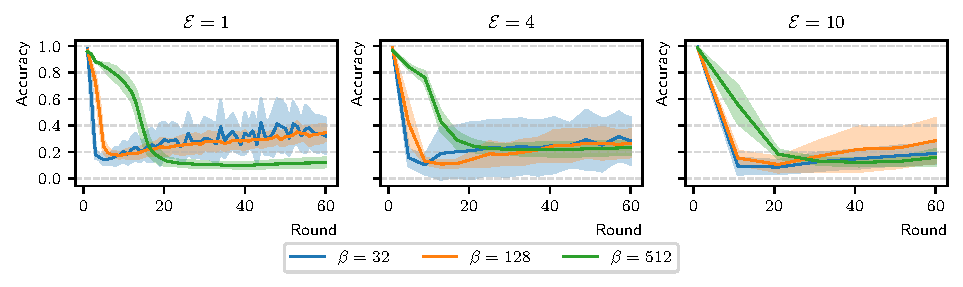
\includegraphics[width=\textwidth]{figures/assessment/hyperparams-late-icdcs.pdf}
    \caption{Effect of the hyperparameters on the accuracy of the poisoned
    model in the late scenario (50\% attackers, CICIDS).}
  \end{figure}

  \begin{itemize}
    \item \texttt{late-3} scenario: attackers start poisoning after 3 rounds
    \item High batch size leads to more inertia, less instantaneous impact
    \begin{itemize}
      \item[$\rightarrow$] More impactful in constrained environments
    \end{itemize}
  \end{itemize}

\end{frame}

\section*{Extra Slides: RADAR}

\begin{frame}
  \sectionpage
\end{frame}

\begin{frame}{The RADAR Architecture}

  \begin{figure}
    \centering
    \includegraphics<1>[width=.7\textwidth]{figures/radar/architecture}
    \includegraphics<2>[width=.7\textwidth]{figures/radar/architecture-xeval}
    \caption{The RADAR architecture.}
  \end{figure}


\end{frame}

\begin{frame}{Results}
  \begin{figure}
    \centering
    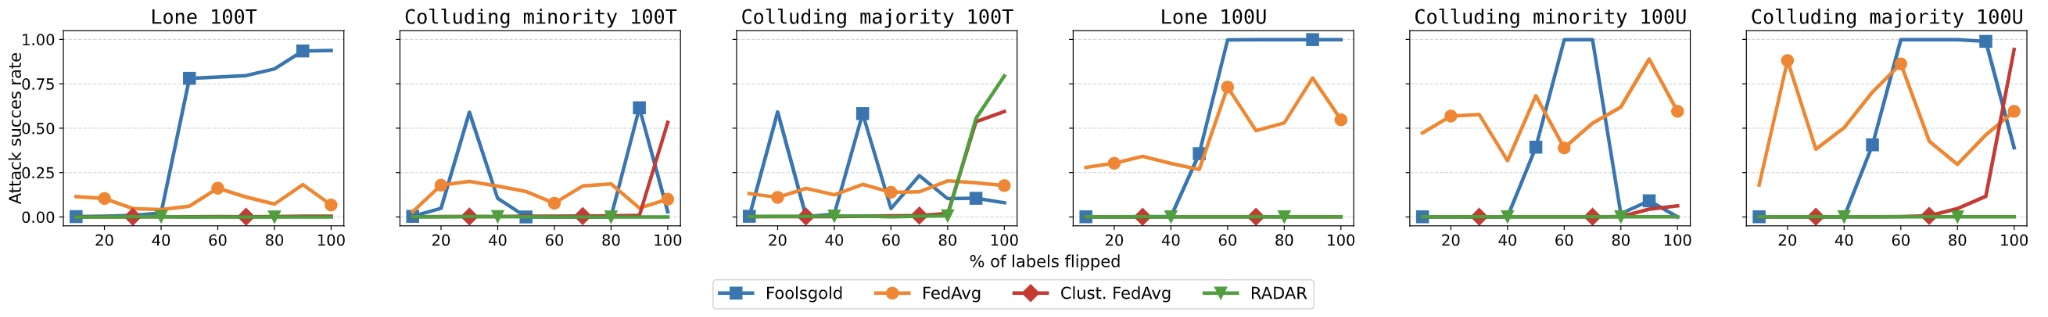
\includegraphics[width=.9\textwidth]{figures/radar/baselines.png}
    \caption{Baseline comparison.}
  \end{figure}
  \begin{figure}
    \centering
    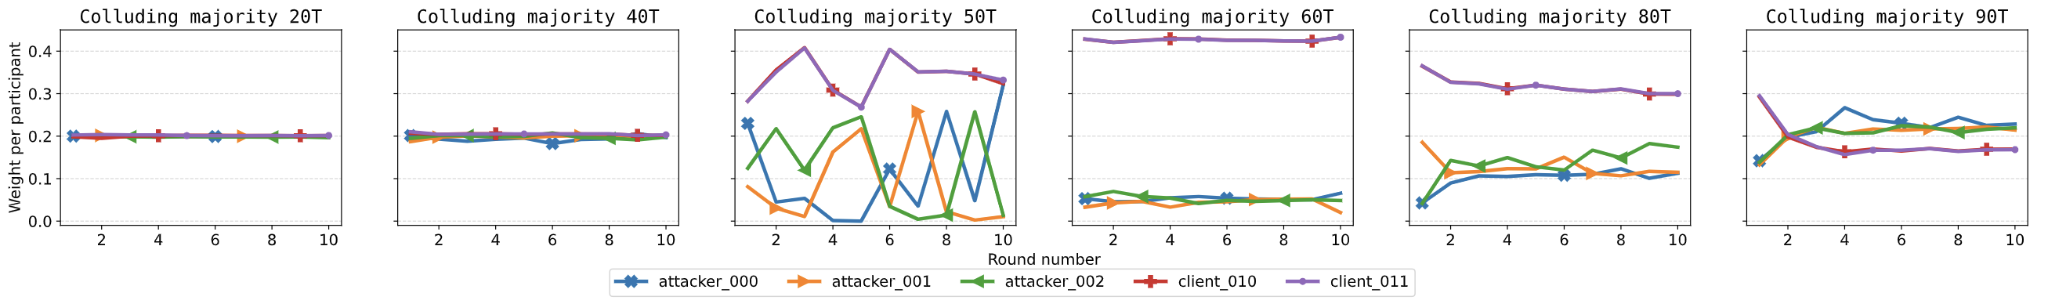
\includegraphics[width=.9\textwidth]{figures/radar/limiting-case.png}
    \caption{RADAR's limiting scenario.}
  \end{figure}
\end{frame}

% ------------------------------------------------------------------------------

\end{document}

%%%%%%%%%%%%%%%%%%%%%%%%%%%%%%%%%%%%%%%%%%%%%%%%%%%%%%%%%%%%%%%%%%%%%%%%%%%%%%%